\documentclass[]{imsart}

\RequirePackage[OT1]{fontenc}
\usepackage{amsthm,amsmath,amssymb,amsfonts,dsfont,mathtools}
\usepackage[colorlinks,citecolor=blue,urlcolor=blue]{hyperref}
\usepackage{tikz}
\usepackage{longtable}
\usepackage{version}
%\usepackage[authoryear]{natbib}
\usepackage{natbib}

\usepackage[babel=true]{csquotes}

%% somes macros
\newcommand{\indep}{\rotatebox[origin=c]{90}{$\models$}}
\newcommand{\1}{\mathds{1}}
\newcommand{\MA}{Y}
\newcommand{\MAO}{\MA^\text{\rm o}}
\newcommand{\MAM}{\MA^\text{\rm m}}
\newcommand{\bMAM}{\mathbf{\MA}^\text{\rm m}}
\newcommand{\bMAO}{\mathbf{\MA}^\text{\rm o}}
\newcommand{\card}[1]{\text{\rm card}\left(#1\right)}

%% sets in SBM
\newcommand{\block}{\mathcal{Q}}

\newcommand{\dyad}{\mathcal{D}}
\newcommand{\dyadO}{\dyad^\text{\rm o}}
\newcommand{\dyadM}{\dyad^\text{\rm m}}

\newcommand{\node}{\mathcal{N}}
\newcommand{\nodeO}{\node^\text{\rm o}}
\newcommand{\nodeM}{\node^\text{\rm m}}

\newcommand{\Pbb}{\mathbb{P}}
\newcommand{\Ebb}{\mathbb{E}}
\newcommand{\Vbb}{\mathbb{V}}
\newcommand{\Rbb}{\mathbb{R}}

% \newcommand{\argmax}{\mathop{\mathrm{arg\ max}}}
% \newcommand{\argmin}{\mathop{\mathrm{arg\ min}}}

%macros
\newcommand{\btau}{\boldsymbol{\tau}}
% \newcommand{\bnu}{\boldsymbol{\nu}}
\newcommand{\bZ}{\mathbf{Z}}
% \newcommand{\bY}{\mathbf{Y}}

% settings
%\pubyear{0000}
%\volume{0}
%\issue{0}
%\firstpage{1}
%\lastpage{8}
% \arxiv{arXiv:0000.0000}

\startlocaldefs
\numberwithin{equation}{section}
\theoremstyle{plain}
\newtheorem{thm}{Theorem}[section]
\newtheorem{dof}[thm]{Definition}
\newtheorem{proposition}[thm]{Proposition}
\newtheorem{corollaire}[thm]{Corollary}
\newtheorem{lemme}[thm]{Lemma}
\newtheorem{property}[thm]{Property}
\theoremstyle{remark}
%\newtheorem{rem}{Remark}[section]
\newtheorem{rem}[thm]{Remark}
\newtheorem{exemple}{Example}
\endlocaldefs

\newcommand{\TT}[1]{\textcolor{red}{ #1}}
\newcommand{\PB}[1]{\textcolor{purple}{#1}}
\newcommand{\MM}[1]{\textcolor{orange}{#1}}
\newcommand{\JC}[1]{\textcolor{blue}{#1}}
%\theoremstyle{plain}
%\newtheorem{theoreme}{Theorem}[section]
%\newtheorem{conjecture}[theoreme]{Conjecture}
%\newtheorem{lemme}[theoreme]{Lemma}
%\newtheorem{proposition}[theoreme]{Proposition}
%\newtheorem{propriete}[theoreme]{Propri\'{e}t\'{e}}
%\newtheorem{corollaire}[theoreme]{Corollary}
%\theoremstyle{definition}
%\newtheorem{definition}[theoreme]{Definition}
%\newtheorem{notation}[theoreme]{Notations}
%\theoremstyle{remark}
%\newtheorem{hypothese}[theoreme]{Hypoth\`{e}se}
%\newtheorem{exemple}[theoreme]{Example}
%\newtheorem{remarque}[theoreme]{Remark}
%\newtheorem{remark}[thm]{Remark}
%\newtheorem{remarquenum}[theoreme]{Remarque num\'{e}rique}
%\newtheorem{rappel}[theoreme]{Rappel}
\newcommand{\proofbegin}{\paragraph{Proof.}\hspace{1em}\\}
\newcommand{\proofend}{\begin{flushright}
$\square$
\end{flushright}}

\newcommand{\loi}{\mathcal{L}}
\newcommand{\Sym}{\text{Sym}}
%%% Notations g\'{e}n\'{e}rales
\newcommand{\dd}{d}
\newcommand{\g}{g}
\newcommand{\q}{\mathcal{Q}}
\newcommand{\ii}{i}
\newcommand{\jj}{j}
\newcommand{\kk}{q}
\newcommand{\el}{\ell}
\newcommand{\m}{m}
\newcommand{\n}{n}
\newcommand{\vrai}{\star}
\newcommand{\al}{\pi}
\newcommand{\als}{\al^\vrai}
\newcommand{\alkl}{\al_{\kk\el}}
\newcommand{\piql}{\pi_{q \el}}
\newcommand{\alskl}{\als_{\kk\el}}
\newcommand{\bal}{\boldsymbol{\al}}
\newcommand{\bals}{\boldsymbol{\al}^\vrai}
\newcommand{\etaa}{\eta}
\newcommand{\etaas}{\eta^\vrai}
\newcommand{\etaaskl}{\etaas_{\kk\el}}
\newcommand{\thetaa}{\theta}
\newcommand{\Thetaa}{\Theta}
\newcommand{\btheta}{\boldsymbol{\thetaa}}
\newcommand{\hbtheta}{\widehat{\btheta}}
\newcommand{\bthetas}{\boldsymbol{\thetaa}^\vrai}
\newcommand{\bTheta}{\boldsymbol{\Thetaa}}
\newcommand{\pii}{\alpha}
\newcommand{\bpi}{\boldsymbol{\pii}}
\newcommand{\pik}{\pii_\kk}
\newcommand{\pisk}{\pis_\kk}
\newcommand{\rhosl}{\rhos_\el}
\newcommand{\bpis}{\boldsymbol{\pii}^\vrai}
\newcommand{\pis}{\pii^\vrai}
\newcommand{\rhos}{\rhoo^\vrai}
\newcommand{\rhoo}{\rho}
\newcommand{\rhol}{\rhoo_\el}
\newcommand{\brho}{\boldsymbol{\rhoo}}
\newcommand{\brhos}{\boldsymbol{\rhoo}^\vrai}
\newcommand{\balphas}{\boldsymbol{\al}^\vrai}
\newcommand{\w}{w}
\newcommand{\bw}{\mathbf{\w}}
\newcommand{\bws}{\bfw^\vrai}
\newcommand{\zjl}{\z_{\jj\el}}
\newcommand{\x}{x}
\newcommand{\y}{y}
\newcommand{\yo}{\y^o\byo}
\newcommand{\bx}{\mathbf{\x}}
\newcommand{\by}{\mathbf{\y}}
\newcommand{\byo}{\mathbf{\y^o}}
\newcommand{\br}{\mathbf{r}}
\newcommand{\xij}{\x_{\ii\jj}}
\newcommand{\yij}{\y_{\ii\jj}}
\newcommand{\X}{X}
\newcommand{\Y}{Y}
\newcommand{\R}{R}
\newcommand{\Xij}{\X_{\ii\jj}}
\newcommand{\Yij}{\Y_{\ii\jj}}
\newcommand{\Rij}{R_{\ii\jj}}
\newcommand{\z}{z}
\newcommand{\bfz}{\mathbf{\z}}
\newcommand{\bz}{\bfz}
\newcommand{\bfw}{\bw}
\newcommand{\bfx}{\bx}
\newcommand{\rij}{\r_{\ii\jj}}
\newcommand{\zik}{\z_{\ii\kk}}
\newcommand{\ziq}{\z_{\ii q}}
\newcommand{\rrij}{r_{\ii \jj}}
\newcommand{\bzs}{\bfz^\vrai}
\newcommand{\wj}{\w_{\jj}}
\newcommand{\zj}{\z_{\jj}}
\newcommand{\zi}{\z_{\ii}}
\newcommand{\lambdaa}{\lambda}
\newcommand{\lamb}{\lambdaa}
\newcommand{\Sal}{\boldsymbol{S}^{\vrai}}
\newcommand{\propcase}{\kappa}
\newcommand{\lambdand}{\lambdaa_{\n,\dd}}
\newcommand{\Salkl}{S^\vrai_{\kk\el}}
\newcommand{\Salmin}{S^\vrai_{\min}}
\newcommand{\Salmax}{S^\vrai_{\max}}


%% Pdf normalit\'{e} asymptotiques
\newcommand{\mcL}{\mathcal{L}}
\newcommand{\mcM}{\mathcal{M}}
\newcommand{\Lc}{\mcL_c}
\newcommand{\prodik}{\prod_{\ii,\kk}}
\newcommand{\prodiq}{\prod_{\ii,q}}
\newcommand{\prodjl}{\prod_{\jj,\el}}
\newcommand{\prodijkl}{\prod_{\ii,\jj,\kk,\el}}
\newcommand{\prodijql}{\prod_{\ii,\jj,q,\el}}
\newcommand{\prodijqlo}{\prod_{\ii, \jj \text{ such as } \yij \in y^{o}, q,\el}}
\newcommand{\prodi}{\prod_{\ii}}
\newcommand{\prodj}{\prod_{\jj}}
\newcommand{\prodij}{\prod_{\ii,\jj}}
\newcommand{\prob}{p}
\newcommand{\Prob}{\mathbb{P}}
\newcommand{\Esp}{\mathbb{E}}
\newcommand{\Var}{\mathbb{V}}
\newcommand{\dens}{\varphi}
\newcommand{\norm}{\psi}
\newcommand{\normp}{\norm'}
\newcommand{\normpm}{(\normp)^{-1}}
\newcommand{\mcZ}{\mathcal{Z}}
\newcommand{\mcW}{\mathcal{W}}
\newcommand{\LL}{\mcL}
\newcommand{\Lam}{\Lambda}
\newcommand{\Lcs}{\Lc^{\vrai}}
\newcommand{\om}{\omega}
\newcommand{\ompi}{\om^{\bpi}}
\newcommand{\omk}{\ompi_{\kk}}
\newcommand{\pikpr}{\pii_{\kk'}}
\newcommand{\omrho}{\om^{\brho}}
\newcommand{\oml}{\omrho_{\el}}
\newcommand{\rholpr}{\rhoo_{\el'}}
\newcommand{\nuu}{\nu}
\newcommand{\nukl}{\nuu_{\kk\el}}
\newcommand{\bompi}{\boldsymbol{\om}^{\bpi}}
\newcommand{\bomrho}{\boldsymbol{\om}^{\brho}}
\newcommand{\bnu}{\boldsymbol{\nu}}
\newcommand{\sommecolonne}{+}
\newcommand{\zsumk}{\z_{\sommecolonne\kk}}
\newcommand{\zsumq}{\z_{\sommecolonne q}}
\newcommand{\zsuml}{\z_{\sommecolonne\el}}
\newcommand{\wsuml}{\w_{\sommecolonne\el}}
\newcommand{\omkpr}{\ompi_{\kk'}}
\newcommand{\oms}{\om^{\vrai}}
\newcommand{\omspi}{\om^{\bpis}}
\newcommand{\omsrho}{\om^{\brhos}}
\newcommand{\omsk}{\omspi_{\kk}}
\newcommand{\omskpr}{\omspi_{\kk'}}
\newcommand{\omsl}{\omsrho_{\el}}
\newcommand{\omslpr}{\omsrho_{\el'}}
\newcommand{\omlpr}{\omrho_{\el'}}
\newcommand{\nus}{\nuu^{\vrai}}
\newcommand{\nuskl}{\nus_{\kk\el}}
\newcommand{\zs}{\z^{\vrai}}
\newcommand{\ws}{\w^{\vrai}}
\newcommand{\zssumk}{\zs_{\sommecolonne\kk}}
\newcommand{\wssuml}{\ws_{\sommecolonne\el}}
\newcommand{\Nskl}{N_{\kk\el;\bzs,\bws}}
\newcommand{\pikc}{\widehat{\pik}^{\Lc}}
\newcommand{\rholc}{\widehat{\rhol}^{\Lc}}
\newcommand{\alklc}{\widehat{\alkl}^{\Lc}}
\newcommand{\Sig}{\Sigma}
\newcommand{\Sigompi}{\Sig_{\omspi}}
\newcommand{\Sigomrho}{\Sig_{\omsrho}}
\newcommand{\ompic}{\widehat{\ompi}^{\Lc}}
\newcommand{\omrhoc}{\widehat{\omrho}^{\Lc}}
\newcommand{\mcN}{\mathcal{N}}
\newcommand{\Signu}{\Sig_{\nus}}
\newcommand{\nuc}{\widehat{\nuu}^{\Lc}}
\newcommand{\muu}{\mu}
\newcommand{\mund}{\muu_{\n,\dd}}
\newcommand{\propcasend}{\propcase_{\n,\dd}}
\newcommand{\xsumsum}{\x_{\sommecolonne\sommecolonne}}
\newcommand{\xsumsumkl}{\x_{\sommecolonne\sommecolonne, \kk\el}}
\newcommand{\piz}{\pii(\bz)}
\newcommand{\hpi}{\hat{\pii}}
\newcommand{\hbpi}{\widehat{\bpi}}
\newcommand{\hbpiz}{\hbpi(\bz)}
\newcommand{\pizs}{\pii(\bzs)}
\newcommand{\rhow}{\rhoo(\bw)}
\newcommand{\hrho}{\widehat{\rhoo}}
\newcommand{\hbrho}{\widehat{\brho}}
\newcommand{\hbrhow}{\hbrho(\bw)}
\newcommand{\rhows}{\rhoo(\bws)}
\newcommand{\pizk}{\widehat{\pii}_{\kk}(\bz)}
\newcommand{\alzq}{\widehat{\al}_{q}(\bz)}
\newcommand{\pizq}{\widehat{\pii}_{q}(\bz)}
\newcommand{\pizsk}{\widehat{\pi}_{\kk}(\bzs)}
\newcommand{\rhowl}{\widehat{\rhoo}_{\el}(\bw)}
\newcommand{\rhowsl}{\widehat{\rhoo}_{\el}(\bws)}
\newcommand{\alzw}{\al(\bz,\bw)}
\newcommand{\pizql}{\widehat{\pi}_{q\el}(\bz)}
\newcommand{\hal}{\widehat{\al}}
\newcommand{\hbal}{\widehat{\bal}}
\newcommand{\hbalzw}{\hbal(\bz,\bw)}
\newcommand{\alzwkl}{\widehat{\al}_{\kk\el}(\bz,\bw)}
\newcommand{\Nkl}{N_{\kk\el;\bz,\bw}}
\newcommand{\barbz}{\overline{\bz}}
\newcommand{\kp}{\kk'}

\def\AArm{\fam0 }%\tenrm}%
\def\R{{\AArm I\!R}}%
\def\un{{\AArm 1\!I}}%

%\newcommand{\R}{R}
\newcommand{\Rg}{\R_{\g}}
\newcommand{\Rm}{\R_{\m}}
\newcommand{\RQ}{\R_{\mathcal{Q}}}
\newcommand{\Rgbz}{\Rg(\bz)}
\newcommand{\Rmbw}{\Rm(\bw)}
\newcommand{\RQbz}{\RQ(\bz)}
\newcommand{\ezw}{e^{(\bz,\bw)}}
\newcommand{\Q}{Q}
\newcommand{\Qnd}{\Q_{\n,\dd}}
\newcommand{\transpose}{{^{T}}}
\newcommand{\vareps}{\varepsilon}
\newcommand{\Bkl}{\boldsymbol{B}_{\kk\el}(\bz,\bw)}
\newcommand{\Nkls}{N_{\kk\el}(\bzs,\bws)}
\newcommand{\ezws}{e^{(\bzs,\bws)}}
\newcommand{\Bkls}{\boldsymbol{B}_{\kk\el}(\bzs,\bws)}
\newcommand{\Rgbzs}{\Rg(\bzs)}
\newcommand{\RQbzs}{\RQ(\bzs)}
\newcommand{\Rmbws}{\Rm(\bws)}
\newcommand{\run}{\rr_{1}}
\newcommand{\rdeux}{\rr_{2}}
\newcommand{\rr}{r}
\newcommand{\Lamb}{\Lambda}
\newcommand{\ttt}{t}
\newcommand{\Salklzw}{\left[S\left(\bz,\bw\right)\right]_{\kk,\el}}
\newcommand{\Salklnd}{S^{\n,\dd}_{\kk,\el}}
\newcommand{\ftau}{\tau}
\newcommand{\Lambtilde}{\tilde{\Lamb}}
\newcommand{\lp}{\el'}
\newcommand{\lambnd}{\lamb_{\n,\dd}}
\newcommand{\zsikp}{\z_{\ii,\kp}^{\vrai}}
\newcommand{\wsjlp}{\w_{\jj,\lp}^{\vrai}}
\newcommand{\alskplp}{\al_{\kp,\lp}^{\vrai}}
\newcommand{\kun}{\kk_{1}}
\newcommand{\kdeux}{\kk_{2}}
\newcommand{\lun}{\el_{1}}
\newcommand{\barx}{\bar{x}}
\newcommand{\hx}{\widehat{\x}}
\newcommand{\hy}{\widehat{\y}}
\newcommand{\hxkl}{\hx_{\kk\el}}
\newcommand{\hxklzw}{\hx_{\kk\el}(\bz, \bw)}
\newcommand{\hyqlz}{\hy_{q\el}(\bz)}
\newcommand{\baral}{\bar{\al}}
\newcommand{\baralkl}{\baral_{\kk\el}}
\newcommand{\barxs}{\barx^\vrai}
\newcommand{\barxkl}{\barx_{\kk\el}}
\newcommand{\barxklzw}{\barx_{\kk\el}(\bz, \bw)}
\newcommand{\barxkplp}{\barx_{\kp\lp}}
\newcommand{\barxkpl}{\barx_{\kp\el}}
\newcommand{\barxskl}{\barxs_{\kk\el}}
\newcommand{\barxskplp}{\barxs_{\kp\lp}}
\newcommand{\entropy}{\mathcal{H}}
\newcommand{\neighborsize}{\kappa}
\newcommand{\vmin}{\underline{\sigma}}
\newcommand{\vmax}{\bar{\sigma}}
\newcommand{\thetasim}{\mathrel{\overset{\btheta}{\sim}}}
\newcommand{\thetassim}{\mathrel{\overset{\bthetas}{\sim}}}
\newcommand{\tnd}{t_{\n\dd}}

%%% Conditional/Profile likelihood
\newcommand{\Fnd}{F_{\n\dd}}
\newcommand{\G}{G}

%%% Notation de Landau
\newcommand{\bigO}{\mathcal{O}}
\newcommand{\smallO}{o}
\newcommand{\Om}{\Omega}

%%% Opérateurs argmin, argmax
\DeclareMathOperator*{\argmin}{arg\!min}
\DeclareMathOperator*{\argmax}{arg\!max}

%% Opérateur Diag
\DeclareMathOperator{\Diag}{Diag}
\DeclareMathOperator{\Trace}{Tr}
\DeclareMathOperator{\Diam}{Diam}
\DeclareMathOperator{\Symmetric}{Sym}
\DeclareMathOperator{\KL}{KL}
\newcommand{\matr}[1]{\boldsymbol{#1}}


%%% Commandes
\newcommand{\norminf}[1]{\left\|#1\right\|_{\infty}}
\newcommand{\mbN}{\mathbb{N}}
\newcommand{\betakl}{\beta_{\kk,\el}}
\newcommand{\kapnd}{\kappa_{\n,\dd}}
\newcommand{\B}{B}
\newcommand{\Bij}{\B_{\ii,\jj}}

\newcommand{\dy}{\text{d\y}}
\newcommand{\dx}{\text{d\x}}
\newcommand{\bY}{\mathbf{\Y}}
\newcommand{\bH}{\mathbf{H}}
\newcommand{\bthetaEMV}{\widehat{\btheta}_{MLE}}
\newcommand{\bpiEMV}{\widehat{\bpi}_{MLE}}
\newcommand{\brhoEMV}{\widehat{\brho}_{MLE}}
\newcommand{\balEMV}{\widehat{\bal}_{MLE}}
\newcommand{\setQ}{\mathbb{Q}}
\newcommand{\Jvar}{J}
\newcommand{\mcH}{\mathcal{H}}
\newcommand{\bthetavar}{\widehat{\btheta}_{var}}
\newcommand{\balvar}{\widehat{\bal}_{var}}
\newcommand{\brhovar}{\widehat{\brho}_{var}}
\newcommand{\bpivar}{\widehat{\bpi}_{var}}
\newcommand{\mcQ}{\mathcal{Q}}
\newcommand{\Sz}{\mathcal{S}_{\bz}}
\newcommand{\Sw}{\mathcal{S}_{\bw}}
\newcommand{\Szs}{\mathcal{S}_{\bzs}}
\newcommand{\Sws}{\mathcal{S}_{\bws}}
\newcommand{\zx}{\widehat{\bz}\left(\bx\right)}
\newcommand{\wx}{\widehat{\bw}\left(\bx\right)}
\newcommand{\Szx}{\mathcal{S}_{\zx}}
\newcommand{\Swx}{\mathcal{S}_{\wx}}

\newcommand{\bthetaMC}{\widehat{\btheta}_{MC}}
\newcommand{\bthetaVAR}{\widehat{\btheta}_{VAR}}
\newcommand{\ICL}{\mbox{ICL}}
\newcommand{\ICLinfi}{\ICL_{\infty}}
\newcommand{\bb}{b}
\newcommand{\sumkl}{\sum_{\kk,\el}}
\newcommand{\Nsklh}{N_{\kk\el;\bzs,\bws}^{h}}
\newcommand{\sumhr}{\sum_{h=1}^{r}}


\begin{document}

\begin{frontmatter}
\title{Consistency and Asymptotic Normality of Stochastic Block Model Estimators under sampling condition}
\runtitle{Consistency and asymptotic normality of SBM estimators under sampling condition}

% \begin{aug}
% \author{\fnms{VINCENT} \snm{BRAULT}\thanksref{a,e1}\ead[label=e1,mark]{vincent.brault@univ-grenoble-alpes.fr}}
% \author{\fnms{CHRISTINE} \snm{KERIBIN}\thanksref{b,e2}\ead[label=e2,mark]{christine.keribin@math.u-psud.fr}}
% \and
% \author{\fnms{MAHENDRA} \snm{MARIADASSOU}\thanksref{c,e3}%
% \ead[label=e3,mark]{mahendra.mariadassou@inra.fr}%
% }
% 
% \address[a]{Univ. Grenoble Alpes, LJK, F-38000 Grenoble, France\\
% CNRS, LJK, F-38000 Grenoble, France
% \printead{e1}}
% 
% \address[b]{Laboratoire de Mathématiques d'Orsay, CNRS, and INRIA Saclay \^Ile de France, Universit\'e Paris-Sud, Universit\'e Paris-Saclay, F-91405 Orsay, France.
% \printead{e2}}
% 
% \address[c]{MaIAGE, INRA, Universit\'e Paris-Saclay, 78352 Jouy-en-Josas, France
% \printead{e3}}
% 
% \runauthor{V. BRAULT et al.}
% 
% \affiliation{Some University and Another University}
% 
% \end{aug}
% 
% \begin{abstract}
% Latent Block Model (LBM) is a model-based method to cluster simultaneously the $d$ columns and $n$ rows of a data matrix. Parameter estimation in LBM is a difficult and multifaceted problem. Although various estimation strategies have been proposed and are now well understood empirically, theoretical guarantees about their asymptotic behavior is rather sparse. We show here that under some mild conditions on the parameter space, and in an asymptotic regime where $\log(\dd)/\n$ and $\log(\n)/\dd$ tend to $0$ when $\n$ and $\dd$ tend to $+\infty$, (1) the maximum-likelihood estimate of the complete model (with known labels) is consistent and (2) the log-likelihood ratios are equivalent under the complete and observed (with unknown labels) models. This equivalence allows us to transfer the asymptotic consistency to the maximum likelihood estimate under the observed model. Moreover, the variational estimator is also consistent. 
% %These results can be used to show that the integrated complete likelihood (ICL) criterion has the same behavior as BIC under the true distribution.
% \end{abstract}

% \begin{keyword}
% \kwd{Stochastic Block Model}
% \kwd{asymptotic normality}
% \kwd{Maximum Likelihood Estimate} \kwd{Concentration Inequality}
% %\kwd{ICL}
% \end{keyword}

\end{frontmatter}

\section{Introduction}

% Coclustering is an unsupervised way to cluster simultaneously the rows and columns of a data matrix, and can be used in numerous applications such as recommendation systems, genomics or text mining. Among the coclustering methods, the Latent Block Model (LBM) is based on the definition of a probabilistic model. 
% 
% We observe a data matrix  $\X=(\xij)$ with $n$ rows and $d$ columns and we suppose that there exists a row-partition with $g$ row-classes and a column-partition with $m$ column-classes.
% The row (resp. column) class for each row (resp. column) is unknown and has to be determined. Once determined, rows and columns can be re-ordered according to this coclustering, to let appear blocks that are  homogeneous and distinct. This leads to a parsimonious data representation. 
% 
% LBM can deal with binary (\cite{govaert2008block}), Gaussian (\cite{lomet2012}), categorical (\cite{keribin2015estimation}) or count (\cite{govaert2010latent}) data. Due to the complex dependence structure, neither the likelihood, nor the computation of the distribution of the assignments conditionally to the observations (E-step of the EM algorithm), and therefore the maximum likelihood estimator (MLE)  are  numerically tractable. Estimation can be however performed either with a variational approximation (leading to an approximate value of the MLE), or with a Bayesian approach (VBayes algorithm or Gibbs sampler). Notice that \cite{keribin2015estimation} recommend to perform a Gibbs sampler combined with a VBayes algorithm. 
% 
% Although these estimation methods give satisfactory results, the consistence and asymptotic normality of the MLE are still an open question. Some partial results exist for LBM, and this question has been solved for SBM (Stochastic Block Model), a special case of LBM where the data is a random graphe  encoded by its adjacency matrix (rows and columns represents the same units, so that there is only one partition, the same for rows and columns). \cite{celisse2012consistency} proved in their Theorem 3 that under the true parameter value, the distribution of the assignments conditionally to the observations of a binary SBM converges to a Dirac of the real assignments. Moreover, this convergence remains valid under the estimated parameter value, assuming that this estimator converges at rate at least $n^{-1}$, where $n$ is the number of nodes (Proposition 3.8). This assumption  is not trivial, and it is not established that such an estimator exists except in some particular cases (\cite{ambroise2012new} for example). \cite{mariadassou2015} presented a unified frame for LBM and SBM in case of observations coming from an exponential family, and showed the consistency of the  assignment conditional distribution under all parameter value in a neighborhood of the true value. \cite{bickel2009nonparametric} and \cite{bickel2013asymptotic} proved the consistency and asymptotic normality of the MLE for the binary SBM. Bursting with the preceding approaches, they first studied the asymptotic behavior of the MLE in the complete model (observations and assignments) which is very simple to handle; then, they showed that the complete likelihood and the marginal likelihood have similar asymptotic behavior by the use of a Bernstein inequality for bounded observations.
% 
% We extend these results to the double asymptotic framework of LBM, following the way of \cite{bickel2013asymptotic}, and for observations coming from some exponential family. Moreover, we introduce the concept of model symmetry  which was not pointed out by these authors, but is necessary to set the asymptotic behavior. The asymptotic normality of the variational estimator is also settled, and an application to model selection criteria is presented.
% 
% The paper is organized as follows. The model, main assumptions and notations are introduced in Section \ref {sec:ModelAndAssumptions}, where model symmetry is also discussed. Section \ref{sec:mle-complete-likelihood} establishes the asymptotic normality of the complete likelihood estimator, and section \ref{sec:profile-likelihood} settles three different types of assignment behaviors. Our main result showing that the observed likelihood behaves like the complete likelihood takes place in section \ref{sec:big-theorem}, and the consistency of MLE and variational estimator is deduced. 
% %We ended with an application to model selection and a discussion on sparsity.
% Technical proofs are gathered in the appendices.

\section{Model and assumptions}

In  SBM,  nodes  from  a  set  $\node  \triangleq  \{1,\dots,n\}$  are
distributed among a set $\block  \triangleq \{1, \dots, Q\}$ of hidden
blocks that  model the latent structure  of the graph. The  blocks are
described  by  categorical  variables $(Z_i,  i\in\node)$  with  prior
probabilities $\alpha  = ( \alpha_{1}, \dots,  \alpha_{Q})$, such that
$\Pbb(Z_i = q) = \alpha_q$,  with $q\in\block$.  
The probability of an edge between any dyad in
$\dyad \triangleq \node \times \node$ only depends on the blocks the
two nodes belong to.  Hence, the presence of an edge between $i$ and
$j$, indicated by the binary variable $Y_{ij}$, is independent on the
other edges conditionally on the latent blocks:
\begin{equation}
\nonumber
\MA_{ij}    \   |    \   Z_i=q,    Z_j   =    \ell   \sim^{\text{ind}}
\dens(., \pi_{q\el}), \qquad \forall (i,j) \in\dyad, \quad \forall
(q,\ell) \in\block\times\block.
\end{equation}
In the
following,
$Y=(Y_{ij})_{i,j\in\dyad}$ is
the $n\times n$ adjacency matrix of the random graph,
$Z = (Z_1, \dots, Z_n)$ the $n$-vector of the latent blocks.  With a slight abuse of notation, we associate to $Z_i$ a vector
of indicator variables $(Z_{i1}, \dots, Z_{iQ})$ such that
$Z_i = q \Leftrightarrow Z_{iq} = 1, Z_{i\ell} = 0$, for all
$\ell \neq q$.  Notice that in the undirected binary case,
$Y_{ij} = Y_{ji}$ for all $(i,j) \in \dyad$ and $Y_{ii} = 0$ for all
$i\in\node$.  Similarly, $\pi_{q\ell}=\pi_{\ell q}$ for all
$(q,\ell)\in\mathcal{Q}\times \mathcal{Q}$. \\

Hence, the  complete parameter set is $\btheta=(\bpi,\bal)\in\bTheta$ and  $\bTheta$  the parameter space.  
% Figure \ref{Fig:notations} summarizes these notations.

% \begin{figure}[!h]
% 

\begin{center}
\begin{tabular}{cc}
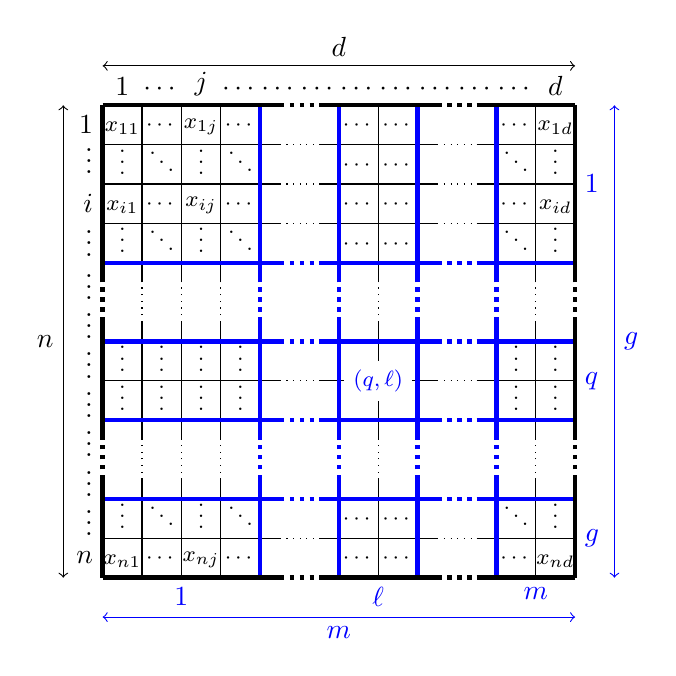
\begin{tikzpicture}
%Petit quadrillage
\foreach  \y in {1.5,2,2.5,4.5,6.5}
\draw (\y,4.75) -- (\y,7);
\foreach  \y in {1.5,2,2.5,4.5,6.5}
\draw (\y,1) -- (\y,2.25);
\foreach  \y in {1.5,2,2.5,4.5,6.5}
\draw (\y,2.75) -- (\y,4.25);
\foreach  \y in {1.5,3.5,5.5,6,6.5}
\draw (1,\y) -- (3.25,\y);
\foreach  \y in {1.5,3.5,5.5,6,6.5}
\draw (3.75,\y) -- (5.25,\y);
\foreach  \y in {1.5,3.5,5.5,6,6.5}
\draw (5.75,\y) -- (7,\y);
%Pointillé
\foreach  \y in {1.5,2,2.5,4.5,6.5}
\draw[dotted] (\y,2.25) -- (\y,2.75);
\foreach  \y in {1.5,2,2.5,4.5,6.5}
\draw[dotted] (\y,4.25) -- (\y,4.75);
\foreach  \y in {1.5,3.5,5.5,6,6.5}
\draw[dotted] (3.25,\y) -- (3.75,\y);
\foreach  \y in {1.5,3.5,5.5,6,6.5}
\draw[dotted] (5.25,\y) -- (5.75,\y);

%Bloc bleu
\foreach  \y in {3,4,5,6}
\draw[ultra thick,color=blue] (\y,4.75) -- (\y,7);
\foreach  \y in {3,4,5,6}
\draw[ultra thick,color=blue] (\y,1) -- (\y,2.25);
\foreach  \y in {3,4,5,6}
\draw[ultra thick,color=blue] (\y,2.75) -- (\y,4.25);
\foreach  \y in {2,3,4,5}
\draw[ultra thick,color=blue] (1,\y) -- (3.25,\y);
\foreach  \y in {2,3,4,5}
\draw[ultra thick,color=blue] (3.75,\y) -- (5.25,\y);
\foreach  \y in {2,3,4,5}
\draw[ultra thick,color=blue] (5.75,\y) -- (7,\y);
%Pointillé
\foreach  \y in {3,4,5,6}
\draw[dotted,ultra thick,color=blue] (\y,2.25) -- (\y,2.75);
\foreach  \y in {3,4,5,6}
\draw[dotted,ultra thick,color=blue] (\y,4.25) -- (\y,4.75);
\foreach  \y in {2,3,4,5}
\draw[dotted,ultra thick,color=blue] (3.25,\y) -- (3.75,\y);
\foreach  \y in {2,3,4,5}
\draw[dotted,ultra thick,color=blue] (5.25,\y) -- (5.75,\y);

%Bord
\foreach  \y in {1,7}
\draw[ultra thick,color=black] (\y,4.75) -- (\y,7);
\foreach  \y in {1,7}
\draw[ultra thick,color=black] (\y,1) -- (\y,2.25);
\foreach  \y in {1,7}
\draw[ultra thick,color=black] (\y,2.75) -- (\y,4.25);
\foreach  \y in {1,7}
\draw[ultra thick,color=black] (1,\y) -- (3.25,\y);
\foreach  \y in {1,7}
\draw[ultra thick,color=black] (3.75,\y) -- (5.25,\y);
\foreach  \y in {1,7}
\draw[ultra thick,color=black] (5.75,\y) -- (7,\y);
%Pointillé
\foreach  \y in {1,7}
\draw[dotted,ultra thick,color=black] (\y,2.25) -- (\y,2.75);
\foreach  \y in {1,7}
\draw[dotted,ultra thick,color=black] (\y,4.25) -- (\y,4.75);
\foreach  \y in {1,7}
\draw[dotted,ultra thick,color=black] (3.25,\y) -- (3.75,\y);
\foreach  \y in {1,7}
\draw[dotted,ultra thick,color=black] (5.25,\y) -- (5.75,\y);

% Les indices en ligne
\draw (1,6.75) node[left]{$1$};
\draw (1,6.4) node[left]{$\vdots$};
\draw (1,5.75) node[left]{$\ii$};
\draw (1,5.35) node[left]{$\vdots$};
\draw (1,1.8) node[left]{$\vdots$};
\draw (1,1.25) node[left]{$\n$};
\draw[<->] (0.5,1) -- (0.5,7);
\draw (0.5,4) node[left]{$\n$};
\foreach  \y in {2.3,2.8,3.3,3.8,4.3,4.8}
\draw (1,\y) node[left]{$\vdots$};

% Les indices en colonnes
\draw (1.25,7) node[above]{$1$};
\draw (1.75,7) node[above]{$\cdots$};
\draw (2.25,7) node[above]{$\jj$};
\draw (2.75,7) node[above]{$\cdots$};
\draw (6.25,7) node[above]{$\cdots$};
\draw (6.75,7) node[above]{$\dd$};
\draw[<->] (1,7.5) -- (7,7.5);
\draw (4,7.5) node[above]{$\dd$};
\foreach  \y in {3.25,3.75,4.25,4.75,5.25,5.75}
\draw (\y,7) node[above]{$\cdots$};

%Cases
\draw (1.25,6.5) node[above]{\footnotesize{$\x_{11}$}};
\draw (1.25,5.5) node[above]{\footnotesize{$\x_{\ii1}$}};
\draw (2.25,6.5) node[above]{\footnotesize{$\x_{1\jj}$}};
\draw (2.25,5.5) node[above]{\footnotesize{$\xij$}};
\draw (1.25,1) node[above]{\footnotesize{$\x_{\n1}$}};
\draw (2.25,1) node[above]{\footnotesize{$\x_{\n\jj}$}};
\draw (6.75,6.5) node[above]{\footnotesize{$\x_{1\dd}$}};
\draw (6.75,5.5) node[above]{\footnotesize{$\x_{\ii\dd}$}};
\draw (6.75,1) node[above]{\footnotesize{$\x_{\n\dd}$}};
%Pointillés
\foreach  \yy in {1.25,2.25,6.75}
\foreach  \y in {6,5,3.5,3,1.5}
\draw (\yy,\y) node[above]{\footnotesize{$\vdots$}};
\foreach  \yy in {1.75,2.75,6.25}
\foreach  \y in {3.5,3}
\draw (\yy,\y) node[above]{\footnotesize{$\vdots$}};
\foreach  \yy in {1.75,2.75,4.25,4.75,6.25}
\foreach  \y in {6.55,5.55,1.05}
\draw (\yy,\y) node[above]{\footnotesize{$\cdots$}};
\foreach  \yy in {4.25,4.75}
\foreach  \y in {6.05,5.05,1.55}
\draw (\yy,\y) node[above]{\footnotesize{$\cdots$}};
\foreach  \yy in {1.75,2.75,6.25}
\foreach  \y in {6,5,1.5}
\draw (\yy,\y) node[above]{\footnotesize{$\ddots$}};

%Indices blocs
\draw[color=blue] (2,1) node[below]{\textbf{$1$}};
\draw[color=blue] (4.5,1) node[below]{\textbf{$\el$}};
\draw[color=blue] (6.5,1) node[below]{\textbf{$\m$}};
\draw[<->,color=blue] (1,0.5) -- (7,0.5);
\draw[color=blue] (4,0.5) node[below]{\textbf{$\m$}};
\draw[color=blue] (7,6) node[right]{\textbf{$1$}};
\draw[color=blue] (7,3.5) node[right]{\textbf{$\kk$}};
\draw[color=blue] (7,1.5) node[right]{\textbf{$\g$}};
\draw[<->,color=blue] (7.5,1) -- (7.5,7);
\draw[color=blue] (7.5,4) node[right]{\textbf{$\g$}};
\draw[color=blue] (4.5,3.5) node[fill=white]{\footnotesize{\textbf{$(\kk,\el)$}}};
\end{tikzpicture}&
%%%%%%%%%%%%%%%%%%%%%%
\hspace{-1cm}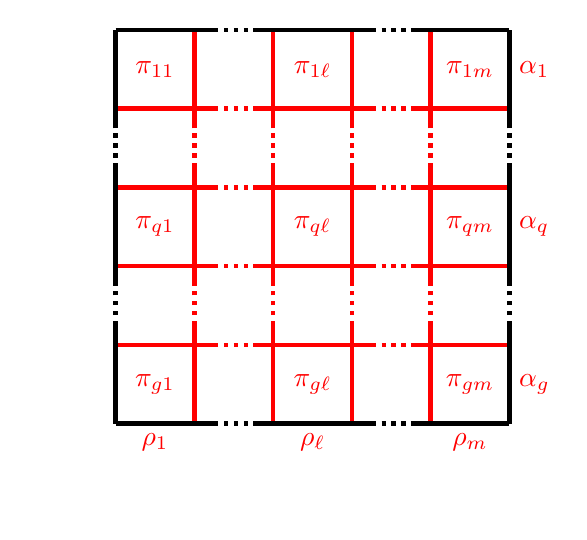
\begin{tikzpicture}

%Bloc bleu
\foreach  \y in {2,3,4,5}
\draw[ultra thick,color=red] (\y,4.75) -- (\y,6);
\foreach  \y in {2,3,4,5}
\draw[ultra thick,color=red] (\y,1) -- (\y,2.25);
\foreach  \y in {2,3,4,5}
\draw[ultra thick,color=red] (\y,2.75) -- (\y,4.25);
\foreach  \y in {2,3,4,5}
\draw[ultra thick,color=red] (1,\y) -- (2.25,\y);
\foreach  \y in {2,3,4,5}
\draw[ultra thick,color=red] (2.75,\y) -- (4.25,\y);
\foreach  \y in {2,3,4,5}
\draw[ultra thick,color=red] (4.75,\y) -- (6,\y);
%Pointillé
\foreach  \y in {2,3,4,5}
\draw[dotted,ultra thick,color=red] (\y,2.25) -- (\y,2.75);
\foreach  \y in {2,3,4,5}
\draw[dotted,ultra thick,color=red] (\y,4.25) -- (\y,4.75);
\foreach  \y in {2,3,4,5}
\draw[dotted,ultra thick,color=red] (2.25,\y) -- (2.75,\y);
\foreach  \y in {2,3,4,5}
\draw[dotted,ultra thick,color=red] (4.25,\y) -- (4.75,\y);

%Bord
\foreach  \y in {1,6}
\draw[ultra thick,color=black] (\y,4.75) -- (\y,6);
\foreach  \y in {1,6}
\draw[ultra thick,color=black] (\y,1) -- (\y,2.25);
\foreach  \y in {1,6}
\draw[ultra thick,color=black] (\y,2.75) -- (\y,4.25);
\foreach  \y in {1,6}
\draw[ultra thick,color=black] (1,\y) -- (2.25,\y);
\foreach  \y in {1,6}
\draw[ultra thick,color=black] (2.75,\y) -- (4.25,\y);
\foreach  \y in {1,6}
\draw[ultra thick,color=black] (4.75,\y) -- (6,\y);
%Pointillé
\foreach  \y in {1,6}
\draw[dotted,ultra thick,color=black] (\y,2.25) -- (\y,2.75);
\foreach  \y in {1,6}
\draw[dotted,ultra thick,color=black] (\y,4.25) -- (\y,4.75);
\foreach  \y in {1,6}
\draw[dotted,ultra thick,color=black] (2.25,\y) -- (2.75,\y);
\foreach  \y in {1,6}
\draw[dotted,ultra thick,color=black] (4.25,\y) -- (4.75,\y);


\draw (0,0) node{ };

%Alpha
\draw[color=red] (1.5,5.5) node{\textbf{$\al_{11}$}};
\draw[color=red] (3.5,5.5) node{\textbf{$\al_{1\el}$}};
\draw[color=red] (5.5,5.5) node{\textbf{$\al_{1\m}$}};
\draw[color=red] (1.5,3.5) node{\textbf{$\al_{\kk1}$}};
\draw[color=red] (3.5,3.5) node{\textbf{$\alkl$}};
\draw[color=red] (5.5,3.5) node{\textbf{$\al_{\kk\m}$}};
\draw[color=red] (1.5,1.5) node{\textbf{$\al_{\g1}$}};
\draw[color=red] (3.5,1.5) node{\textbf{$\al_{\g\el}$}};
\draw[color=red] (5.5,1.5) node{\textbf{$\al_{\g\m}$}};

%Rho
\draw[color=red] (1.5,1) node[below]{\textbf{$\rhoo_{1}$}};
\draw[color=red] (3.5,1) node[below]{\textbf{$\rhol$}};
\draw[color=red] (5.5,1) node[below]{\textbf{$\rhoo_{\m}$}};

%pi
\draw[color=red] (6,5.5) node[right]{\textbf{$\pii_{1}$}};
\draw[color=red] (6,3.5) node[right]{\textbf{$\pik$}};
\draw[color=red] (6,1.5) node[right]{\textbf{$\pii_{\g}$}};


\end{tikzpicture}\\
\end{tabular}
\end{center}

% \caption{\label{Fig:notations} Notations. Left: Notations for the elements of observed data matrix are in black, notations for the block clusters are in blue. Right: Notations for the model parameter.}
% \end{figure}

When performing inference from data, we note $\bthetas = (\bpis, \bals)$ the true parameter set, \emph{i.e.} the parameter values used to generate the data, and $\bzs$ the true (and usually unobserved) assignment of rows and columns to their group.
For given matrices of indicator variables $\bz$, we also note:
\begin{itemize}
\item $\zsumk = \sum_{\ii} \zik$ 
\item $\zssumk$ his counterpart for $\bzs$.
\end{itemize}
The confusion matrix allows to compare the partition.
\begin{dof}[confusion matrix]
  \label{def:confusion}
  For given assignments $\bz$ and $\bzs$, we define the \emph{confusion matrix} between $\bz$ and $\bzs$, noted $\RQbz$, as follows:
  \begin{equation}
    \label{eq:confusion-matrix}
    \RQbz_{q q^{\prime}} = \frac{1}{\n} \sum_{\ii} \z^\vrai_{\ii q} \z_{\ii q^{\prime}}
  \end{equation}
\end{dof}


\subsection{Missing data for SBM}

Regarding SBM inference, a missing value corresponds to a missing entry in the adjacency matrix $\MA$, typically denoted by \texttt{NA}'s.
Therefore, $\MA$ has three possible entries $0$, $1$ or \texttt{NA}.
We rely on the $n\times n$ sampling matrix $R$ to record the data sampled during this process:
\begin{equation}
\label{eq:R}
 (R_{ij}) = \begin{cases}
  1 &   \text{ if $\MA_{ij}$  is observed,}  \\
  0 &   \text{ otherwise.}  \\
\end{cases}
\end{equation}
As  a  shortcut,  we use  $\MAO  =  \{\MA_{ij}  :  R_{ij} =  1\}$  and
$\MAM=\{\MA_{ij} :  R_{ij} =  0 \}$  to denote  the sets  of variables
respectively    associated    with     the    \textit{observed}    and
\textit{missing} data.  The \emph{sampling  design} is the description
of the stochastic process that generates  $R$.  It is assumed that the
network pre-exists this process, which is fully characterized by the
conditional distribution $p_\psi(R|\MA)$, the parameters of which are
such   that   $\psi$   and   $\theta$   live   in   a   product   space
$\Theta   \times   \Psi$.    We    then   follow   the   framework   of
\citet{Rubin1976} for  missing data that  we adapt to the  presence of
the latent variables $Z_i$: the  joint probability density function of
the observed data satisfies
\begin{equation}
p_{\theta, \psi}(\MAO,R)=\int \int p_{\theta}(\MAO,\MAM,Z)p_\psi(R|\MAO,\MAM,Z)d\MAM dZ.
\label{eq:likelihood}
\end{equation}
Simplifications may  occur in  \eqref{eq:likelihood} depending  on the
sampling  design, leading  to the  three usual  types of  missingness:
Missing completely  at random (MCAR),  Missing at random (MAR)  or Not
missing  at random  (NMAR).  For  SBM,  this typology  depends on  the
relations between  the network $Y$,  the latent structure $Z$  and the
sampling  $R$,  so  that  the missingness  is  characterized  by  four
directed acyclic graphs (DAG) displayed in Figure~\ref{fig:DAGs}.
Since the network pre-exists the sampling process, we do not consider DAG where
$R$ is a parent node.

%\begin{figure}[htbp!]
%  \centering
%  \begin{tabular}{c@{\hspace{1.5em}}c@{\hspace{1.5em}}c@{\hspace{1.5em}}c}
%    \begin{tikzpicture}
%      \tikzstyle{every edge}=[-,>=stealth',shorten >=1pt,auto,thin,draw]
%      \tikzstyle{every state}=[draw=none,text=white,scale=0.8, font=\scriptsize, transform shape]
%      \node[state,fill=blue!40!black] (Z) at (0,0) {Z};
%      \node[state,fill=yellow!60!orange] (\MA) at (1.25,0) {\MA};
%      \node[state,fill=red!60!black] (R) at (2.5,0) {R};
%      \draw[->,>=latex] (Z) -- (\MA);
%      %    \draw[->,>=latex] (\MA) -- (R);
%    \end{tikzpicture}
%    &
%    \begin{tikzpicture}
%      \tikzstyle{every edge}=[-,>=stealth',shorten >=1pt,auto,thin,draw]
%      \tikzstyle{every state}=[draw=none,text=white,scale=0.8, font=\scriptsize, transform shape]
%      
%      \node[state,fill=blue!40!black] (Z) at (0,0) {Z};
%      \node[state,fill=yellow!60!orange] (\MA) at (1.25,0) {\MA};
%      \node[state,fill=red!60!black] (R) at (2.5,0) {R};
%      
%      \draw[->,>=latex] (Z) -- (\MA);
%      \draw[->,>=latex] (\MA) -- (R);
%    \end{tikzpicture}
%    & 
%      \begin{tikzpicture}
%        
%        \tikzstyle{every edge}=[-,>=stealth',shorten >=1pt,auto,thin,draw]
%        \tikzstyle{every state}=[draw=none,text=white,scale=0.8, font=\scriptsize, transform shape]
%        \tikzstyle{every node}=[fill=red!80!black]
%        
%        \node[state,fill=blue!40!black] (Z) at (0,0) {Z};
%        \node[state,fill=yellow!60!orange] (\MA) at (1.25,0) {\MA};
%        \node[state,fill=red!60!black] (R) at (2.5,0) {R};
%        
%        \draw[->,>=latex] (Z) -- (\MA);
%        \draw[->,>=latex] (\MA) -- (R);
%        \draw[->,>=latex] (Z) to[bend left] (R);
%        
%      \end{tikzpicture}
%    &
%      \begin{tikzpicture}
%        
%        \tikzstyle{every edge}=[-,>=stealth',shorten >=1pt,auto,thin,draw]
%        \tikzstyle{every state}=[draw=none,text=white,scale=0.8, font=\scriptsize, transform shape]
%        \tikzstyle{every node}=[fill=green!50!black]
%        
%        \node[state,fill=blue!40!black] (Z) at (0,0) {Z};
%        \node[state,fill=yellow!60!orange] (\MA) at (-2/2,-2/2) {\MA};
%        \node[state,fill=red!60!black] (R) at (2/2,-2/2) {R};
%        
%        \draw[->,>=latex] (Z) -- (\MA);
%        \draw[->,>=latex] (Z) -- (R);
%      \end{tikzpicture}
%    \\
%    (a) & (b) & (c) & (d) \\
%  \end{tabular}    
%  \caption{DAGs of relationships between $Y,Z$ and $R$ considered in
%    the framework of missing data  for SBM. Notice the systematic edge
%    between $Z$ and $Y$ which comes from the SBM.
% DAG (a)  corresponds to MCAR,  DAG (b) can  correspond to MAR  or NMAR
% (additional specifications are necessary) while  DAGs (c) and (d) lead
% to NMAR.
%}
%	\label{fig:DAGs}
%\end{figure}


The type of  missingness for SBM  can be
defined as follows:
\begin{equation}
  \label{def:missingness}
  \text{Sampling design for SBM is }
  \begin{cases}
    \text{MCAR} & \text{if } R \ \indep \ (\MAM, Z, \MAO),\\
    \text{MAR} & \text{if } R \ \indep \ (\MAM,Z) \ | \ \MAO,\\
    \text{NMAR} & \text{otherwise}.\\
  \end{cases}
\end{equation}
% \begin{definition}[MAR, MCAR, NMAR]
%   A sampling design is MAR, respectively MCAR, if the sampling process
%   $R$ is such that
%   \begin{equation*}
%     R \ \indep \ (\MAM,Z) \ | \ \MAO, \qquad \text{resp. } \quad R \ \indep \ (\MAM, Z, \MAO). 
%   \end{equation*}
%   Otherwise, the sampling design is NMAR.
% \end{definition}
% It is straightforward that MCAR is a special case of MAR.

\begin{property}\label{prop:mar} According to definition
  \eqref{def:missingness}, if the sampling design is MAR, then maximising $p_{\theta, \psi}(\MAO,R)$  in $\theta$  is equivalent  to maximising $p_{\theta}(\MAO)$ in $\theta$, this corresponds to ignorability notion defined in Rubin and recalled in  Handcock and Gile.
\label{MAR}
\end{property}

\subsection{Sampling design examples}

\begin{dof}[Random dyad sampling]
  Each   dyad    $(i,j)   \in\dyad$    has   the    same   probability
  $\Pbb(R_{ij}=1)=\rho$ to be observed independently on the others.
\end{dof}
\begin{dof}[Star sampling]
  Each   node    $i   \in \{1,...n\}$    has   the    same   probability
  $\Pbb(S_{i}=1)=\rho$ to be observed independently on the others.
\end{dof}
These designs  are trivially MCAR because  each dyad/node is sampled  with the
same probability $\rho$ which does not depend on $Y$. \\

\begin{proposition}
Under random dyad sampling, defining $N_i = \sum_{j \neq i}R_{ij}$ and $\Omega_{0,n} = \{ \forall i \in \{ 1, ..., n \}, \ N_i \geqslant 1 \}$. Then 
$$\mathbb{P}\left(\underset{n\to+\infty}{\lim}\Omega_{0,n}\right) = 1.$$
\label{prop:Omega}
\end{proposition}
\begin{proof}
Noticing that $N_i \sim \text{Bin}(n, \rho)$, then  $\mathbb{P}(N_i \geqslant 1) = 1 - {\rho}^n$. As a consequence
$\mathbb{P}(\overline{\Omega_{0,n}}) \leqslant  \sum_{i} \mathbb{P}(N_i = 0) = n\rho^n \underset{n\to+\infty}{\longrightarrow} 0$, and 
$\mathbb{P}(\Omega_{0,n}) \underset{n\to+\infty}{\longrightarrow} 1$. Then
$\mathbb{P}(\limsup (\overline{\Omega_{0,n}})) = 0$ by Borel-Cantelli theorem (because $\sum_{n} \mathbb{P}(\overline{\Omega_{0,n}})$ does not converge), and as
$\overline{\limsup \overline{\Omega_{0,n}}} = \overline{\bigcap_{n \geqslant 0} \bigcup_{q \geqslant n} \overline{\Omega_{0,n}}} = \bigcup_{n \geqslant 0} \bigcap_{q \geqslant n} {\Omega_{0,n}} =
\liminf {\Omega_{0,n}}$, the result follow.
\end{proof}

\begin{rem}
Proposition \ref{prop:Omega} is trivially true for any node-centered sampling design.
\end{rem}

In the following we will consider only MCAR samplings dyad-centered. Because of proposition \ref{prop:Omega}, we will always consider that at least one dyad is sampled for each node of the network.


\subsection{Likelihood}
When the labels are known, the {\em complete log-likelihood} is given by:
\begin{equation}
  \label{eq:log-vraisemblance-complete}
  \begin{aligned}
    \Lc(\bz;\btheta)&= \log\prob(\byo,\bz;\btheta)\\
    &= \log\left\{ \left(\prodiq{\pii^{\ziq}}\right)\left(\prodijql{\dens\left(\yij;\piql\right)^{\ziq\zjl\rrij}}\right) \right\}\\
    &= \log\left\{ \left(\prodi{\pii_{\zi}}\right)\left(\prodij{\dens\left(\yij;\pi_{\zi\zj}\right)^{\rrij}}\right) \right\}.	\\
  \end{aligned}
\end{equation}
But the labels are usually unobserved, and the {\em observed log-likelihood} is obtained by marginalization over all the label configurations:
\begin{equation}
  \label{eq:log-vraisemblance-observee}
  \LL(\btheta)=\log\prob(\byo;\btheta) = \log \left( \sum_{\bz \in \mcZ}\prob(\byo,\bz;\btheta) \right).
\end{equation}

\subsection{Assumptions}\label{sec:assumptions}
We focus here on parametric models where $\dens$ belongs to a regular one-dimension exponential family in canonical form:
\begin{equation}
  \dens(x, \pi) = b(x)\exp(\pi x - \norm(\pi)),
\end{equation}
where $\pi$ belongs to the space  $\mathcal{A}$, so that $\dens(\cdot, \pi)$ is well defined for all $\pi \in \mathcal{A}$. Classical properties of exponential families insure that $\norm$ is convex, infinitely differentiable on $\mathring{\mathcal{A}}$, that $\normpm$ is well defined on $\normp(\mathring{\mathcal{A}})$. When $X_{\pi} \sim \dens(., \pi)$, $\Esp[X_\pi] = \normp(\pi)$ and $\Var[X_{\pi}] = \normp'(\pi)$. \\

%\subsection{Hypothèses sur le paramètre}
Moreover, we make the following assumptions on the parameter space~:
\begin{enumerate}
% \item $\bTheta$ is compact \textcolor{red}{is it necessary?};
\item[$H_1$]: There exist a positive constant $c$, and a compact $C_\pi$ such that 
  \begin{equation*}
%   \label{eq:assumptions}
    \bTheta \subset [c, 1-c]^{\q} \times C_{\pi}^{\q \times \q} \quad \text{with} \quad C_\pi \subset \mathring{\mathcal{A}}.
  \end{equation*}
\item[$H_2$]: The true parameter $\bthetas = (\bpis, \bals)$ lies in the relative interior of $\bTheta$.
\item[$H_3$]: The map $\pi \mapsto \dens(\cdot, \pi)$ is injective.
\item[$H_4$]: 
Each row and each column of $\bals$ is unique.
%\item The ratio $\log(\dd)/\n$ (resp. $\log(\n)/\dd$) tend to 0 with $\n$ and $\dd$.
\end{enumerate}
%\begin{rem}

The previous assumptions are standard. Assumption~$H_1$ ensure that the group proportions are bounded away from $0$ and $1$ so that no group disappears when $\n$ goes to infinity. It also ensures that $\pi$ is bounded away from the boundaries of the $\mathcal{A}$ and that there exists a $\kappa>0$, such that $[\piql - \neighborsize, \piql + \neighborsize] \subset \mathring{\mathcal{A}}$ for all parameters $\piql$ of $\btheta \in \bTheta$. Assumptions $H_3$ and $H_4$ are necessary to ensure that the model is identifiable. If the map $\pi \mapsto \dens(., \pi)$ is not injective, the model is trivially not identifiable. Similarly, if rows $q$ and $q^\prime$ are identical, we can build a more parsimonious model that induces the same distribution of $\by$ by merging groups $q$ and $q^\prime$. In the following, we  consider that $\mathcal{Q}$, the number of classes (or groups) is known.

%\end{rem}
Moreover, we define the $ \delta(\bal)$, that captures the differences between groups: lower values means that there are two classes that are very similar. 
\begin{dof}[class distinctness]
  \label{def:group-distinctness}
  For $\btheta = (\bpi, \bal) \in \bTheta$. We define:
  \begin{equation*}
    \delta(\bal) =  \min_{\el, \lp} \max_{q} \KL(\piql, \pi_{q \lp}) 
  \end{equation*}
  with $\KL(\pi,\pi') = \Esp_{\pi}[\log(\dens(X, \pi)/\dens(X, \pi'))]=\normp(\pi) (\pi - \pi') + \norm(\pi') - \norm(\pi)$ the Kullback divergence between $\dens(., \pi)$ and $\dens(., \pi')$, when $\dens$ comes from an exponential family.
\end{dof}
\begin{rem}
Since all $\bal$ have distinct rows and columns, $\delta(\bpi) > 0$.
\end{rem}

\begin{rem}
Since we restricted $\pi$ in a bounded subset of $\mathring{\mathcal{A}}$, there exists two positive values $M_{\pi}$ and $\neighborsize$ such that $C_\pi + (-\neighborsize, \neighborsize) \subset [-M_{\pi}, M_\pi] \subset \mathring{\mathcal{A}}$. Moreover, the variance of $\X_{\pi}$ is bounded away from $0$ and $+\infty$. We note
\begin{equation}
  \label{eq:condition-variance}
  \sup_{\pi \in [-M_{\pi}, M_{\pi}] } \Var(\X_\pi) = \vmax^2 < +\infty \quad \text{and} \quad \inf_{\pi \in [-M_{\pi}, M_{\pi}]} \Var(\X_\pi) = \vmin^2 > 0.
\end{equation}
\end{rem}
\begin{proposition}
With the previous notations, if $\pi \in C_\pi$ and $X_{\pi} \sim \dens(., \pi)$, then $X_\pi$ is subexponential with parameters $(\vmax^2, \neighborsize^{-1})$.
\end{proposition}

\begin{rem}
These assumptions are satisfied for many distributions, including but not limited to:
\begin{itemize}
\item Bernoulli, when the proportion $p$ is bounded away from $0$ and $1$, or natural parameter $\pi = \log(p / (1 - p))$ bounded away from $\pm \infty$;
\item Poisson, when the mean $\lambda$ is bounded away from $0$ and $+\infty$, or natural parameter $\pi = \log(\lambda)$ bounded away from $\pm \infty$;
\item Gaussian with known variance when the mean $\mu$, which is also the natural parameter, is bounded away from $\pm \infty$.
\end{itemize}
In particular, the conditions stating that $\norm$ is twice differentiable and that $\normpm$ exists are equivalent to assuming that $\X_{\pi}$ has positive and finite variance for all values of $\pi$ in the parameter space.
\end{rem}


%\begin{rem}
%For the sake of simplicity, we only consider data matrices where most elements $\Xij$ are non-zero. Similar results are available for "zero-inflated" distributions $\X_{\al} \sim \kappa_{\n, \dd}\delta_0 + (1 - \kappa_{\n, \dd})\dens(., \al)$ where  $\kappa_{\n, \dd} \xrightarrow[\n,\dd \to +\infty]{} 0$. If missing values are treated as $0$, the two configurations correspond to dense and sparse data tables. Results concerning zero-inflated distributions are detailed in Section~\ref{sec:sparsity}.
%\end{rem}




\subsection{Symmetry}
\label{sec:definitions}
The study of the asymptotic properties of the MLE will lead to take into account symmetry properties on the parameter set. We first recall the definition of a permutation, then define equivalence relationships for assignments and parameter, and  precise symmetry. 

\begin{dof}[permutation]
  \label{def:permutation}
  Let $s$ be a permutation on $\{1,\dots,\g\}$ and $t$ a permutation on $\{1,\dots,\m\}$. If $\boldsymbol{A}$ is a matrix with $\g$ columns, we define $\boldsymbol{A}^s$ as the matrix obtained by permuting the columns of $\boldsymbol{A}$ according to $s$, \emph{i.e.} for any row $\ii$ and column $\kk$ of $\boldsymbol{A}$, ${A}^s_{\ii \kk} = A_{\ii s(\kk)}$. If $\boldsymbol{B}$ is a matrix with $\m$ columns and $\boldsymbol{C}$ is a matrix with $\g$ rows and $\m$ columns, $\boldsymbol{B}^t$ and $\boldsymbol{C}^{s,t}$ are defined similarly:
  \begin{equation*}
    \boldsymbol{A}^s = \left( A_{\ii s^{}(\kk)} \right)_{\ii,\kk} \quad  \boldsymbol{B}^t = \left( B_{\jj t^{}(\el)} \right)_{\jj, \el} \quad \boldsymbol{C}^{s,t} = \left( C_{s^{}(\kk) t^{}(\el)} \right)_{\kk,\el}
  \end{equation*}
\end{dof}

\begin{dof}[equivalence]
  \label{def:equivalence}
  We define the following equivalence relationships:
  \begin{itemize}
  \item Two assignments $\bz$ and $\bz'$ are \emph{equivalent}, noted $\sim$, if they are equal up to label permutation, \emph{i.e.} it exists a permutation $s$ such that $\bz' = \bz^s$.
  \item Two parameters are $\btheta$ and $\btheta'$ are \emph{equivalent}, noted $\sim$, if they are equal up to label permutation, \emph{i.e.} it exists a permutation $s$ such that $(\bpi^s,\bal^{s}) = (\bpi', \bal')$. This is \emph{label-switching}.
  \item  $(\btheta, \bz)$ and $(\btheta', \bz')$ are \emph{equivalent}, noted $\sim$, if they are equal up to label permutation on $\bal$, \emph{i.e.} it exists a permutation $s$ such that $(\bal^{s}, \bz^s) = (\bal', \bz')$.
  \end{itemize}
\end{dof}

\begin{dof}[distance]
  \label{def:equivalence-distance}
  We define the following distance, up to equivalence, between configurations $\bz$ and $\bzs$:
    \begin{equation*}
    \|\bz - \bzs\|_{0, \sim} = \inf_{\bz' \sim \bz} \|\bz' - \bzs\|_0
    \end{equation*}
    where, for all matrix $\bz$, we use the Hamming norm $\left\|\cdot\right\|_{0}$ defined by
\[\left\|\bz\right\|_{0}=\sum_{\ii,\kk}{\mathds{1}{\left\{\zik\neq0\right\}}}.\]
\end{dof}
  
  
The last equivalence relationship is not concerned with $\bal$. It is useful when dealing with the conditional likelihood $\prob(\bx| \bz; \btheta)$ which does not depend on $\bal$ :  in fact, if $(\btheta, \bz) \sim (\btheta', \bz')$, then for all $\bx$, we have $\prob(\bx| \bz; \btheta) = \prob(\bx| \bz'; \btheta')$. 
Note also that $\bz \sim \bzs$  if and only if the confusion matrix $\RQbz$  is equivalent to a diagonal matrix. 

\begin{dof}[symmetry]
  \label{def:symmetry}
  We say that the parameter $\btheta$ \emph{exhibits symmetry for the permutation} $s$ if
  \begin{equation*}
    (\bpi^s, \bal^{s}) = (\bpi, \bal).
  \end{equation*}
  $\btheta$ \emph{exhibits symmetry} if it exhibits symmetry for any non trivial pair of permutations $(s,t)$. Finally the set of pairs $(s,t)$ for which $\btheta$ exhibits symmetry is noted $\Symmetric(\btheta)$.
\end{dof}

%\begin{dof}[$\btheta$-symmetry]
%  \label{def:theta-symmetry}
%  For any $\btheta \in \bTheta$, we say that assignments $(\bz, \bw)$ and $(\bz', \bw')$ are \emph{$\btheta$-equivalent}, noted $\thetasim$, if there exists $(s,t) \in \Symmetric(\btheta)$ such that $(\bz^s, \bw^t) = (\bz', \bw')$. \CK{ ou est-ce qu'on s'en sert?}
%\end{dof}

\begin{rem}
  The set of parameters that exhibit symmetry is a manifold of null Lebesgue measure in $\bTheta$.  The notion of symmetry allows us to deal with a notion of non-identifiability of the class labels that is subtler than and different from label switching.\\
% To emphasize the difference between equivalence and symmetry, consider the following model: $\bpi = (1/2, 1/2)$, $\brho = (1/3, 2/3)$ and $\bal = \left( \begin{array}{cc} \al_1 & \al_2 \\ \al_2 & \al_1 \end{array} \right) $ with $\al_1 \neq \al_2$. The only permutations of interest here are $s = t = [1\ 2]$. Choose any $\bz$ and $\bw$. Because of label switching, we know that $\prob(\bx, \bz^s, \bw^t; \btheta^{s,t}) = \prob(\bx, \bz, \bw; \btheta)$. $(\bz^s, \bw^t)$ and $(\bz, \bw)$ have the same likelihood but under \emph{different} parameters $\btheta$ and $\btheta^{s,t}$. If however, $\brho = (1/2, 1/2)$, then $(s, t) \in \Symmetric(\btheta)$ and $\btheta^{s,t} = \btheta$ so that $(\bz, \bw)$ and $(\bz^s, \bw^t)$ have exactly the same likelihood under the \emph{same} parameter $\btheta$. In particular, if $(\bz, \bw)$ is a maximum-likelihood assignment under $\btheta$, so is $(\bz^s, \bw^t)$. In other words, if $\theta$ exhibits symmetry,  the maximum-likelihood \emph{assignment} is not unique under the true model and there are at least $\# \Symmetric(\btheta)$ of them. 
\end{rem}




%%%%%%%%%%%%%%%%%%%%%%%%%%%%%%%%%%%%%%%%%%
%%%%% Complete model
%%%%%%%%%%%%%%%%%%%%%%%%%%%%%%%%%%%%%%%%%%
\section{Asymptotic properties in the complete data model}
\label{sec:mle-complete-likelihood}
As stated in the introduction, we first study the asymptotic properties of the complete data model.
Let $\widehat{\btheta}_{c}=\left(\hbpi,\hbal\right)$ be the MLE of $\btheta$ in the complete data model, where the real assignments $\bz=\bzs$ are known. We can derive the following general estimates from Equation~\eqref{eq:log-vraisemblance-complete}:

\begin{equation}
  \label{eq:mle-complete-likelihood}
  \begin{aligned}
    \hpi_{q}  = \pizq = \frac{\zsumq}{\n}&& \\
    \hyqlz = \frac{\sum_{\ii < \jj} \yij \rrij \ziq \zjl}{\sum_{\ii < \jj} \rrij \ziq \zjl} & \quad
    \hal_{q\el}  = \pizql = \normpm \left(  \hyqlz \right)&
  \end{aligned}
\end{equation}

\begin{lemme}
$$U_{n} = \frac{1}{\binom{n}{2}}\sum_{\ii < \jj} \rrij \ziq \zjl \xrightarrow[\n \to +\infty]{\mathbb{P}} \rho \pii_{\kk}\pii_{l}$$
\label{lem:convdenom}
\end{lemme}
\begin{proof}
Noticing that $\mathbb{E}[\rrij \ziq \zjl] = \rho \pii_{\kk}\pii_{l}$ and defining $q_{i,j}^{q, \el}=\rrij \ziq \zjl - \rho \pii_{\kk}\pii_{l}$. By Hoeffding decomposition for U-statistics (see \cite{Hoeffding1963})
\begin{equation}
 \label{eq:ustat}
 U_{n} = \frac{1}{n!}\sum_{\sigma \in \mathfrak{S}_{n}}\frac{1}{\lfloor\frac{n}{2}\rfloor}\sum_{i=1}^{\lfloor\frac{n}{2}\rfloor}q_{\sigma(i), \sigma(i+\lfloor\frac{n}{2}\rfloor)}^{q, \el},
\end{equation}
where for each permutation $\sigma \in \mathfrak{S}$, $\sum_{i=1}^{\lfloor\frac{n}{2}\rfloor}q_{\sigma(i), \sigma(i+\lfloor\frac{n}{2}\rfloor)}^{q, \el}$ is a sum of independant r.v. Then, for $\gamma > 0$ by Jensen's inequality and Hoeffding's lemma about bounded r.v.
\begin{eqnarray*}
\mathbb{E}\left[ \exp(\gamma U_{n}) \right] &\leq& \frac{1}{n!}\sum_{\sigma \in \mathfrak{S}_{n}}\mathbb{E}\exp\left(\frac{\gamma}{\lfloor\frac{n}{2}\rfloor}\sum_{i=1}^{\lfloor\frac{n}{2}\rfloor}q_{\sigma(i), \sigma(i+\lfloor\frac{n}{2}\rfloor)}^{q, \el}\right) \\
&\leq& \exp\left(\frac{\gamma^2}{8\lfloor\frac{n}{2}\rfloor}\right).
\end{eqnarray*}
Finally, using the same proof than Hoeffding's allows us to conclude.
\end{proof}



\begin{proposition}
  \label{prop:mle-asymptotic-normality}
  The matrix $\Sigma_{\bpis} = \Diag(\bpis) - \bpis\left(\bpis\right)\transpose $is semi-definite positive, of rank $\mathcal{Q}-1$, and $\widehat{\bpi}$ is asymptotically normal:
  \begin{equation}
    \label{eq:mle-proportion-asymptotic-normality}
    \sqrt{\n}\left( \hat{\bpi}\left(\bzs\right) - \bpis \right) \xrightarrow[\n \to \infty]{\mathcal{D}} \mathcal{N}(0, \Sigma_{\bpis})
  \end{equation}
Similarly, let $V(\bals)$ be the matrix defined by $[V(\bals)]_{q \el} = 1/\normp'(\pi^\vrai_{q\el})$ and\\  $\Sigma_{\bals} = \rho^{-1}\Diag^{-1}(\bpis) V(\bals) \Diag^{-1}(\bpis)$. Then:
  \begin{equation}
    \label{eq:mle-parameters-asymptotic-normality}
    \sqrt{\n(\n-1)/2}\;(\hal_{q\el}\left(\bzs\right) - \pi^\vrai_{q\el}) \xrightarrow[\n, \to \infty]{\mathcal{D}}  \mathcal{N}(0, \Sigma_{\bals, q \el})\;\;\; \hbox{for all  } q, \el
  \end{equation}
  where the components are independent. 
\end{proposition}

\textit{Proof:}
Since $\hat{\bpi}\left(\bzs\right) = \left(\hpi_1\left(\bzs\right), \dots, \hpi_\g\left(\bzs\right)\right)$ is the sample mean of $\n$ i.i.d. multinomial random variables with parameters $1$ and $\bpis$, a simple application of the central limit theorem (CLT) gives:
\begin{equation*}
  \Sigma_{\bpis, \kk \kp} =
  \begin{cases}
    \pii^{\vrai}_{\kk}(1 - \pii^{\vrai}_{\kk}) & \text{if} \quad \kk = \kp \\
    -\pii^{\vrai}_{\kk} \pii^{\vrai}_{\kp} & \text{if} \quad \kk \neq \kp \\
  \end{cases}
\end{equation*}
which proves Equation~\eqref{eq:mle-proportion-asymptotic-normality}
where $\Sigma_{\bpis}$ is
semi-definite positive of rank $\mathcal{Q} - 1$.

Similarly, $\normp\left(\hal_{\kk\el}\left(\bzs\right)\right)$ is
the average of $\sum_{\ii < \jj} \rrij \ziq^\star \zjl^\star$
i.i.d. random variables with mean
$\normp\left(\al^\vrai_{\kk\el}\right)$ and variance
$\normp'\left(\al^\vrai_{\kk\el}\right)$. $\sum_{\ii < \jj} \rrij \ziq^\star \zjl^\star$
is itself random but thanks to lemma \ref{lem:convdenom} : 
\mbox{$\frac{1}{\binom{n}{2}}\sum_{\ii < \jj} r_{ij} \ziq^\star \zjl^\star \xrightarrow[\n \to +\infty]{\mathbb{P}} p \pii^\vrai_{\kk}\pii^\vrai_{l}$}. Therefore, by Slutsky's lemma and
the CLT for random sums of random variables \cite{Shanthikumar1984}, we have:
\begin{eqnarray*}
&&\sqrt{\frac{\n(\n-1)}{2}\rho\pii^\star_{\kk}\pii^\star_{\el}} \left(\normp\left(\hal_{\kk\el}\left(\bzs\right)\right) - \normp(\al^\vrai_{\kk\el}) \right)  \\
&& = \sqrt{\frac{\n(\n-1)}{2}\rho\pii^\star_{\kk}\pii^\star_{\el}} \left( \frac{\sum_{\ii < \jj} \Xij \Rij \zik^{\vrai} \zjl^{\vrai}}{\sum_{\ii < \jj} \Rij \ziq^\star \zjl^\star} - \normp(\al^\vrai_{\kk\el}) \right) \\
&& \xrightarrow[\n,\dd \to +\infty]{\mathcal{D}} \mcN\left(0, \normp'(\al^\vrai_{\kk\el})\right)
\end{eqnarray*}
The differentiability of $\normpm$ and the delta method then gives:
\begin{equation*}
  \sqrt{\frac{\n(\n-1)}{2}} \left(\hal_{\kk\el}\left(\bzs\right) - \al^\vrai_{\kk\el} \right) \xrightarrow[\n,\dd \to +\infty]{\mathcal{D}} \mcN\left(0, \frac{1}{\rho\pii^\star_{\kk}\rhoo^\star_{\el} \normp'(\al^\vrai_{\kk\el})}\right)
\end{equation*}
and the independence results from the independence of $\hal_{\kk\el}\left(\bzs\right)$ and
$\hal_{\kp\lp}\left(\bzs\right)$ as soon as $\kk \neq \kp$ or $\el
\neq \lp$, as they involve different sets of i.i.d. variables.

\begin{flushright}
$\square$
\end{flushright}

\begin{proposition}[Local asymptotic normality]\label{prop:LocalAsymp}
Let $\Lcs$ the function defined on $\bTheta$ by $\Lcs\left(\bpi,\bal\right)=\log\prob\left(\by^o,\bzs;\btheta\right)$. For any $s$, $t$ and $u$ in a compact set, we have:
\begin{eqnarray*}
\Lcs\left(\bpis+\frac{s}{\sqrt{\n}},\bals+\frac{u}{\sqrt{\frac{\n(\n-1)}{2}}}\right)
&=&\Lcs\left(\bthetas\right) + s\transpose\bY_{\bpis}+ \text{Tr}(u\transpose\bY_{\bals})\\
& -&\left(\frac{1}{2}s\transpose\Sig_{\bpis}s+\frac{1}{2} \text{Tr}\left((u \odot u)\transpose\Sig_{\bals}\right)\right)\\
&+&o_{P}(1)\\
\end{eqnarray*}
where $\odot$ denote the Hadamard product of two matrices (element-wise product) and $\Sig_{\bpis}$, $\Sig_{\brhos}$ and $\Sig_{\bals}$ are defined in Proposition~\ref{prop:mle-asymptotic-normality}. $\bY_{\bpis}$, $\bY_{\brhos}$ are asymptotically Gaussian with zero mean and respective variance matrices $\Sig_{\bpis}$, $\Sig_{\brhos}$ and $\bY_{\bals}$ is a matrix of asymptotically independent Gaussian components with zero mean and variance matrix $\Sig_{\bals}$.
\end{proposition}
\proofbegin
By Taylor expansion,
\begin{eqnarray*}
& &\!\!\!\!\!\!\!\!\!\!\Lcs\left(\bpis+\frac{s}{\sqrt{\n}},\bals+\frac{u}{\sqrt{\frac{\n(\n-1)}{2}}}\right)\\
&=&\Lcs\left(\bthetas\right)+\frac{1}{\sqrt{\n}}s\transpose\nabla{\Lcs}_{\bpi}\left(\bthetas\right) +\frac{1}{\sqrt{\frac{\n(\n-1)}{2}}}\text{Tr}\left(u\transpose\nabla{\Lcs}_{\bal}\left(\bthetas\right)\right)\\
&&\quad+\frac{1}{\n}s\transpose\bH_{\bpi}\left(\bthetas\right)s+\frac{1}{\frac{\n(\n-1)}{2}}\text{Tr}\left((u \odot u)\transpose\bH_{\bal}\left(\bthetas\right)\right)+o_{P}(1)\\
\end{eqnarray*}
where $\nabla{\Lcs}_{\bpi}\left(\bthetas\right)$ and $\nabla{\Lcs}_{\bal}\left(\bthetas\right)$ denote the respective components of the gradient of $\Lcs$ evaluated at $\bthetas$ and $\bH_{\bpi}$ and $\bH_{\bal}$ denote the conditional hessian of $\Lcs$ evaluated at $\bthetas$. By inspection, $\bH_{\bpi}/\n$ and $\bH_{\bal}/\frac{\n(\n-1)}{2}$ converge in probability to constant matrices and the random vectors $\nabla{\Lcs}_{\bpi}\left(\bthetas\right)/\sqrt{\n}$ and $\nabla{\Lcs}_{\bal}\left(\bthetas\right)/\sqrt{\frac{\n(\n-1)}{2}}$ converge in distribution by central limit theorem. %This concludes the proof.
\proofend


%%%%%%%%%%%%%%%%%%%%%%%%%%%%%
\section{Profile Likelihood}
\label{sec:profile-likelihood}
%%%%%%%%%%%%%%%%%%%%%%%%%%%%%
To study the likelihood behaviors, we shall work conditionally to the real configurations $\bzs$ that have enough observations in each group. We therefore define regular configurations which occur with high probability, then introduce conditional and profile log-likelihood ratio. 
\subsection{Regular assignments}
\begin{dof}[$c$-regular assignments]
  \label{def:regular}
  Let $\bz \in \mcZ$. For any $c > 0$, we say that $\bz$ is c-\emph{regular} if
  \begin{equation}
    \label{eq:regular-configuration}
    \min_{\kk} \zsumk \geq {c\n} .
  \end{equation}
\end{dof}



In regular configurations, each group  has $\Om(\n)$ members, where $u_\n=\Om(\n)$ if there exists two constant $a, b>0$ such that for $\n$ enough large $a\n \leq u_\n \leq b\n$. $c/2$-regular assignments, with $c$ defined in Assumption $H_1$, have high  $\Prob_{\bthetas}$-probability in the space of all assignments, uniformly over all $\bthetas \in \bTheta$. 

Each $\zsumk$ is a sum of $\n$ i.i.d Bernoulli r.v. with parameter $\pik \geq \pii_{\min} \geq c$. A simple Hoeffding bound shows that
\begin{equation*}
  \Prob_{\bthetas}\left( \zsumk \leq \n \frac{c}{2} \right)
  \leq
  \Prob_{\bthetas}\left( \zsumk \leq \n \frac{\pik}{2} \right)
  \leq
  \exp\left( - 2\n\left(\frac{\pik}{2}\right)^2 \right)
  \leq
  \exp\left( - \frac{\n c^2}{2} \right)
\end{equation*}
taking a union bound over $\q$ values of $\kk$ lead to Proposition \ref{cor:prob-regular-configurations-star}.
\begin{proposition}
  \label{cor:prob-regular-configurations-star}
  Define $\mcZ_1$ as the subset of $\mcZ$ made of $c/2$-regular assignments, with $c$ defined in assumption $H_1$. Note $\Om_1$ the event $\{ \bzs
  \in \mcZ_1 \}$, then:
  \begin{equation*}
    \Prob_{\bthetas}\left( \bar{\Om}_1 \right) \leq \q \exp\left( -\frac{\n c^2}{2}\right).
  \end{equation*}
\end{proposition}

We define now balls of configurations taking into account equivalent assignments classes.
\begin{dof}[Set of local assignments]
  \label{prop:small-deviations-profile-likelihood}
  We note $S(\bzs, r)$ the set of configurations that have a representative (for $\sim$) within relative radius $r$ of $\bzs$:
  \begin{equation*}
    S(\bzs, r) = \left\{ \bz : \|\bz - \bzs\|_{0, \sim} \leq r \n \right\}
  \end{equation*}
\end{dof}

\subsection{Conditional and profile log-likelihoods}
\label{sec:cond-and-prof-likelihood} 
%We now consider the likelihood $\prob(\bx,\bz,\bw;\btheta)$ when $\bz$ and $\bw$ are unknown. Instead of maximizing this quantity for the correct assignments $(\bzs, \bws)$, we will maximize it in $\btheta$ it for \enquote{well-behaved} test assignments $(\bz, \bw)$ and show that it is a $\smallO_P$ of $\prob(\bx,\bzs,\bws;\bthetas)$ whenever $(\bz, \bw) \nsim (\bzs, \bws)$.
%
We first introduce few notations.

\begin{dof}
\label{def:conditional-profile-likelihood}
We define the conditional log-likelihood ratio $F_{\n}$ and its expectation $G$ as:
\begin{equation}
  \label{eq:conditional-likelihood}
  \begin{aligned}
    \Fn(\btheta, \bz) & = \log \frac{\prob(\byo | \bz;\btheta)}{\prob(\byo | \bzs;\bthetas)} \\
    \G(\btheta, \bz) & = \Esp_{\bthetas} \left[ \left. \log \frac{\prob(\byo | \bz;\btheta)}{\prob(\byo | \bzs;\bthetas)} \right| \bzs  \right] \\
  \end{aligned}
\end{equation}
We also define the profile log-likelihood ratio $\Lamb$ and its expectation $\Lambtilde$ as:
\begin{equation}
  \label{eq:profile-likelihood}
  \begin{aligned}
    \Lamb(\bz) & = \max_{\btheta} \Fn(\btheta, \bz)  \\
    \Lambtilde(\bz) & = \max_{\btheta} \G(\btheta, \bz).
  \end{aligned}
\end{equation}
\end{dof}

\begin{rem}
As  $\Fn$ and $\G$ only depend on $\btheta$ through $\bal$, we will sometimes replace $\btheta$ with $\bal$ in the expressions of $\Fn$ and $\G$. Replacing $F_{\n}$ and $G$ by their profiled version $\Lamb$ and $\Lambtilde$ allows us to get rid of the continuous argument of $\Fn$ and to effectively use discrete contrasts $\Lamb$ and $\Lambtilde$.
\end{rem}

The following proposition shows which values of $\bal$ maximize $\Fn$ and $\G$ to attain $\Lamb$ and $\Lambtilde$.
\begin{proposition}[maximum of $\G$ and $\Lambtilde$ in $\theta$]
\label{prop:profile-likelihood}
Conditionally on  $\bzs$, define
the following quantities:
\begin{equation}
  \label{eq:profile-likelihood-notations}
  \begin{aligned}
    \Sal & = (\Salkl)_{\kk\el} = \left( \normp(\alskl) \right)_{\kk\el} \\
    \barykl(\bz) & = \Esp_{\bthetas}[\hyklz | \bzs] = \frac{\left[ \RQbz\transpose \Sal \RQbz \right]_{\kk\el}}{\pizk\pizl}
  \end{aligned}
\end{equation}
with $\barykl(\bz)=0$ for $\bz$ such that $\pizk=0$ or $\pizl=0$. 
Then $\Fnd(\btheta, \bz)$ and $\G(\btheta, \bz)$ are maximum in $\bal$ for  $\hbal(\bz)$ and $\bar{\bal}(\bz)$ defined by:
\begin{equation*}
  \hal(\bz)_{\kk\el} = \normpm ( \hyklz ) \quad \text{and} \quad \bar{\al}(\bz)_{\kk\el} = \normpm ( \barykl(\bz) )
\end{equation*}
so that
\begin{equation*}
  \begin{aligned}
    \Lamb(\bz) & = \Fn(\hbal(\bz), \bz) % = \sum_{\kk} \sum_{\el} \pizk \rhowl \nu(\hxklzw) - \sum_{\kk} \sum_{\el} \pizsk \rhowsl \nu(\Salkl) \\
    \\
    \Lambtilde(\bz) & = \G(\bar{\bal}(\bz), \bz) % = \sum_{\kk} \sum_{\el} \pizk \rhowl \nu(\barxklzw) - \sum_{\kk} \sum_{\el} \pizsk \rhowsl \nu(\Salkl).
  \end{aligned}
\end{equation*}
\end{proposition}
Note that although $\bar{y}_{\kk\el} = \mathbb{E}_{\bthetas}\left[\left.\hat{y}_{\kk\el}\right|\bzs\right]$, in general %$\bar{\al}_{\kk\el} = \normpm(\barxkl) \neq \normpm(\hxkl) = \hat{\al}_{\kk\el}$
$\bar{\al}_{\kk\el} \neq \mathbb{E}_{\bthetas}\left[\left.\hat{\al}_{\kk\el}\right|\bzs\right]$ by non linearity of $\normpm$. Nevertheless, $\normpm$ is Lipschitz over compact subsets of $\normp(\mathring{\mathcal{A}})$ and therefore, with high probability, $|\bar{\al}_{\kk\el} - \hat{\al}_{\kk\el}|$ and $|\hykl - \barykl|$ are of the same order of magnitude. 

The maximum and $\argmax$ of $G$ and $\Lambtilde$ are characterized by the following propositions.
\begin{proposition}[maximum of $\G$ and $\Lambtilde$ in $(\theta,\bz)$]
  \label{prop:maximum-conditional-likelihood}
  Let $\KL(\al,\al') = \normp(\al) (\al - \al') + \norm(\al') - \norm(\al)$ be the Kullback divergence between $\dens(., \al)$ and $\dens(., \al')$ then:
  \begin{equation}
    \label{eq:conditional-likelihood-second-form}
    \G(\btheta, \bz) = - \rho\n^2 \sum_{\kk,\kp} \sum_{\el,\lp} \RQbz_{\kk,\kp} \RQbz_{\el, \lp} \KL(\al^\vrai_{\kk\el}, \al_{\kp\lp}) \leq 0.
  \end{equation}
  Conditionally on the set $\Om_1$ of regular assignments and for $n> 2/c$,
\begin{itemize}
\item[(i)] $\G$ is maximized at $(\bals, \bzs)$ and its equivalence class.
\item[(ii)] $\Lambtilde$ is maximized at $(\bzs)$ and its equivalence class; moreover, $\Lambtilde(\bzs)=0$.
\item[(iii)] The maximum of $\Lambtilde$ (and hence the maximum of $\G$) is well separated.
\end{itemize}



\end{proposition}
Property $(iii)$ of Proposition \ref{prop:maximum-conditional-likelihood} is a direct consequence of the local upperbound for $\Lambtilde$ as stated as follows:

\TT{Jusqu'ici tout est bon pour moi, la proposition suivante est � v�rifier.}

\begin{proposition}[Local upperbound for  $\Lambtilde$]
\label{prop:profile-likelihood-derivative}
Conditionally upon $\Om_1$, there exists a positive constant $C$ such that for all $\bz \in S(\bzs, C)$:
\begin{equation}
\label{eq:conditional-likelihood-separability}
  \Lambtilde(\bz) \leq -\frac{c\delta(\bals)}{4}  \n \|\bz - \bzs\|_{0, \sim}
\end{equation}
\end{proposition}
Proofs of Propositions \ref{prop:profile-likelihood}, \ref{prop:maximum-conditional-likelihood} and \ref{prop:profile-likelihood-derivative} are reported in Appendix \ref{sec:proofPL}.

\section{Main Result}
\label{sec:big-theorem}
%%%%%%%%%%%%%%%%%%%%%%
We are now ready to present our main result
stated in Theorem \ref{thm:observed-akin-to-complete-general}.

\begin{thm}[complete-observed]
  \label{thm:observed-akin-to-complete-general}
  Consider that assumptions $H_1$ to $H_4$ hold for the Latent Block Model of known order with $n\times d$ observations coming from an univariate exponential family  and define  $\# \Symmetric(\btheta)$ as the set of pairs of permutation $(s,t)$ for which $\btheta=(\bpi,\brho,\bal)$ exhibits symmetry. Then, for $n$ and $d$ tending to infinity with asymptotic rates  $\log (\dd)/\n\rightarrow 0$ and $\log(\n)/\dd\rightarrow 0$, the observed likelihood ratio behaves like the complete likelihood ratio, up to a bounded multiplicative factor:
  \begin{equation*}
    \frac{\prob(\bx; \btheta)}{\prob(\bx; \bthetas)} = \frac{\# \Symmetric(\btheta)}{\# \Symmetric(\bthetas)} \max_{\btheta' \sim \btheta} \frac{\prob(\bx, \bzs, \bws; \btheta')}{\prob(\bx, \bzs, \bws; \bthetas)}\left(1 + \smallO_P(1)\right) + \smallO_P(1)
  \end{equation*}
  where the $\smallO_P$ is uniform over all $\btheta \in \bTheta$.
\end{thm}
The maximum over all $\btheta'$ that are equivalent to $\btheta$ stems from the fact that because of label-switching, $\btheta$ is only identifiable up to its $\sim$-equivalence class from the observed likelihood, whereas it is completely identifiable from the complete likelihood.\\
As already pointed out, if $\bTheta$ exhibits symmetry, the maximum likelihood assignment is not unique under the true model, and $\# \Symmetric(\btheta)$ terms contribute with the same weight. This was not taken into account by \cite{bickel2013asymptotic}.
The next corollary is deduced immediately~:
\begin{corollaire}
  \label{cor:observed-akin-to-complete-simple-case}
  If $\bTheta$ contains only parameters that do not exhibit symmetry:
  \begin{equation*}
    \frac{\prob(\bx; \btheta)}{\prob\left(\bx; \btheta^{\vrai}\right)} = \max_{\btheta' \sim \btheta} \frac{\prob(\bx, \bzs, \bws; \btheta')}{\prob(\bx, \bzs, \bws; \bthetas)}\left(1 + \smallO_P(1)\right) + \smallO_P(1)
  \end{equation*}
where the $\smallO_P$ is uniform over all $\bTheta$.
\end{corollaire}


%\textcolor{red}{Redondant avec la fin de la section~\ref{sec:cond-and-prof-likelihood}?}
Using the conditional log-likelihood, the observed likelihood can be written as
\begin{eqnarray}
\nonumber
\prob(\bx; \btheta) &=&
  \sum_{ (\bz, \bw)} \prob(\bx, \bz, \bw; \btheta) \\
%  &=&  \prob(\bx| \bzs, \bws; \bthetas) \sum_{(\bz, \bw)} 
% \prob(\bz, \bw; \btheta)\frac{\prob(\bx| \bz,\bw;\btheta)}{\prob(\bx| \bzs,\bws;\bthetas)}\\
%
&=&\prob(\bx| \bzs, \bws; \bthetas)
\sum_{(\bz, \bw)}   \prob(\bz, \bw; \btheta) \exp(\Fnd(\btheta, \bz, \bw) ).
\end{eqnarray} 
%Hence, the convergence of $\Fnd$ is of crucial importance to study the asymptotic of the observed likelihood. In fact, we shall have to study it for three types of configurations

The proof proceeds with an examination of the asymptotic behavior of  $\Fnd$ on three types of configurations that partition $\mcZ\times\mcW$:


\begin{enumerate}
\item  \emph{global control}: for $(\bz, \bw)$ such that $\Lambtilde(\bz, \bw) = \Omega(-\n\dd)$, Proposition \ref{prop:conditional-likelihood-convergence} proves a large deviation behavior for $\Fnd = -\Omega_P(\n\dd)$  and in turn those assignments contribute a $\smallO_{P}$ of $\prob(\bx, \bzs, \bws; \bthetas))$ to the sum (Proposition \ref{prop:large-deviations-profile-likelihood}). 

\item \emph{local control}: a small deviation result (Proposition~\ref{prop:profile-likelihood-convergence-local}) is needed  to show that the combined contribution of assignments close to but not equivalent to $(\bzs, \bws)$ is also a $\smallO_{P}$ of $\prob(\bx, \bzs, \bws; \bthetas)$ (Proposition \ref{prop:small-deviations-profile-likelihood}). 
\item \emph{equivalent assignments}: Proposition~\ref{prop:equivalent-configurations-profile-likelihood} examines which of the remaining assignments, all equivalent to $(\bzs, \bws)$, contribute to the sum.
\end{enumerate}
These results are presented in next section \ref{sec:technicalpropositions} and their proofs reported in Appendix \ref{sec:proofPL}. They are then put together in section \ref{sec:proofbigth} to achieve the proof of our main result. The remainder of the section is devoted to the asymptotics of the ML and variational estimators as a consequence of the main result.

\subsection{Different asymptotic behaviors}\label{sec:technicalpropositions}

We begin with a large deviations inequality for configurations $(\bz, \bw)$ far from $(\bzs, \bws)$ and leverage it to prove that far away configurations make a small contribution to $\prob(\bx; \btheta)$. 

\subsubsection{Global Control}
% a global deviation bound for $\Fnd$ and shows that  $\left( \Fnd - \G \right)_{+} = \bigO_{P}(\sqrt{\n\dd})$.

\begin{proposition}[large deviations of $\Fn$]
  \label{prop:conditional-likelihood-convergence}
  Let $\Diam(\bTheta) = \sup_{\btheta, \btheta'} \|\btheta - \btheta' \|_{\infty}$. For all $\vareps_{\n, \dd} < \neighborsize / (2\sqrt{2}\Diam(\bTheta))$ and $\n, \dd$ large enough that 
  \begin{multline}
    \label{eq:conditional-likelihood-convergence}
    \Delta_{\n\dd}^1(\vareps_{\n\dd})\\ = \Prob\left( \sup_{\btheta, \bz, \bw} \left\{ \Fnd(\btheta, \bz, \bw) - \Lambtilde(\bz,\bw) \right\} \geq \vmax \n\dd \Diam(\bTheta) 2\sqrt{2}\vareps_{\n\dd}\left[1 + \frac{\g\m}{2\sqrt{2\n\dd}\vareps_{\n\dd}} \right] \right) \\ 
    \leq \g^{\n} \m^{\dd} \exp\left( - \frac{\n\dd\vareps_{\n\dd}^2} {2}\right)
  \end{multline}
\end{proposition}

\begin{proposition}[contribution of global assignments]
  \label{prop:large-deviations-profile-likelihood}
  Assume $\log(\dd)/n \to 0$, $\log(\n)/\dd \to 0$ when $n$ and $\dd$ tend to infinity, and choose $\tnd$ decreasing to $0$ such that $\tnd \gg \max(\frac{\n+\dd}{\n\dd}, \frac{\log(\n\dd)}{\sqrt{\n\dd}})$. Then conditionally on $\Omega_1$ and for $\n,\dd$ large enough that $2\sqrt{2\n\dd}\tnd \geq \g\m$, we have:
  \begin{equation*}
    \sup_{\btheta \in \bTheta} \sum_{(\bz, \bw) \notin S(\bzs, \bws, \tnd)} \prob(\bz, \bw, \bx; \btheta) = \smallO_P( \prob(\bzs, \bws, \bx; \bthetas) )
  \end{equation*}
\end{proposition}

\subsubsection{Local Control}

Proposition~\ref{prop:conditional-likelihood-convergence} gives deviations of order $\bigO_{P}(\sqrt{\n\dd})$, which are only useful for $(\bz, \bw)$ such that $\G$ and $\Lambtilde$ are large compared to $\sqrt{\n\dd}$. For $(\bz, \bw)$ close to $(\bzs, \bws)$, we need tighter concentration inequalities, of order $\smallO_P(-(\n+\dd))$, as follows:

\begin{proposition}[small deviations $\Fnd$]
  \label{prop:profile-likelihood-convergence-local}
  Conditionally upon $\Om_1$, there exists three positive constant $c_1$, $c_2$ and $C$ such that for all $\vareps \leq \neighborsize \vmin^2$, for all $(\bz, \bw) \nsim(\bzs, \bws)$ such that $(\bz, \bw) \in S(\bzs, \bws, C)$:
  \begin{equation}
    \label{eq:profile-likelihood-convergence-local}
    \begin{aligned}
      \Delta_{\n\dd}^2(\vareps) = \Prob_{\bthetas}\left( \sup_{\btheta} \frac{\Fnd(\btheta, \bz, \bw) - \Lambtilde(\bz, \bw)}{\dd \| \bz - \bzs \|_{0, \sim} + \n \| \bw - \bws \|_{0, \sim}} \geq \vareps \right) \leq \exp \left( - \frac{\n\dd c^2 \vareps^2}{128(c_1 \vmax^2 + c_2 \neighborsize^{-1} \vareps)}\right)
    \end{aligned}
  \end{equation}
\end{proposition}

The next propositions builds on Proposition~\ref{prop:profile-likelihood-convergence-local} and \ref{prop:maximum-conditional-likelihood} to show that the combined contributions of assignments close to $(\bzs, \bws)$ to the observed likelihood is also a $\smallO_P$ of  $\prob(\bzs, \bws, \bx; \bthetas)$

\begin{proposition}[contribution of local assignments]
  \label{prop:small-deviations-profile-likelihood}
  With the previous notations
  \begin{equation*}
    \sup_{\btheta \in \bTheta} \sum_{\substack{(\bz, \bw) \in S(\bzs, \bws, C) \\ (\bz, \bw) \nsim (\bzs, \bws)}} \prob(\bz, \bw, \bx; \btheta) = \smallO_P( \prob(\bzs, \bws, \bx; \bthetas) )
  \end{equation*}
\end{proposition}


\subsubsection{Equivalent assignments}
It remains to study the contribution of equivalent assignments.
\begin{proposition}[contribution of equivalent assignments]
  \label{prop:equivalent-configurations-profile-likelihood}
  For all $\btheta \in \bTheta$, we have 
  \begin{equation*}
    \sum_{(\bz, \bw) \sim (\bzs, \bws)} \frac{\prob(\bx, \bz, \bw; \btheta)}{\prob(\bx, \bzs, \bws; \bthetas)} = \# \Symmetric(\btheta) \max_{\btheta' \sim \btheta} \frac{\prob(\bx, \bzs, \bws; \btheta')}{\prob(\bx, \bzs, \bws; \bthetas)} (1 + \smallO_P(1))
  \end{equation*}   
  where the $\smallO_P$ is uniform in $\btheta$. 
\end{proposition}

\subsection{Proof of the main result}\label{sec:proofbigth}

\proofbegin We work conditionally on $\Omega_1$. Choose $(\bzs, \bws)
\in \mcZ_1\times \mcW_1$ and a sequence $\tnd$ decreasing to $0$ but satisfying $\tnd \gg \max\left(\frac{\n+\dd}{\n\dd}, \frac{\log(\n\dd)}{\sqrt{\n\dd}}\right)$ (this is possible since $\log(\dd)/\n\rightarrow 0$ and $\log(\n)/\dd\rightarrow 0$). According to Proposition~\ref{prop:large-deviations-profile-likelihood}, 
\begin{equation*}
    \sup_{\btheta \in \bTheta} \sum_{(\bz, \bw) \notin S(\bzs, \bws, \tnd)} \prob(\bz, \bw, \bx; \btheta) = \smallO_P( \prob(\bzs, \bws, \bx; \bthetas) )
\end{equation*}
Since $\tnd$ decreases to $0$, it gets smaller than $C$ (used in proposition~\ref{prop:small-deviations-profile-likelihood}) for $\n, \dd$ large enough. As this point, Proposition~\ref{prop:small-deviations-profile-likelihood} ensures that:
\begin{equation*}
    \sup_{\btheta \in \bTheta} \sum_{\substack{(\bz, \bw) \in S(\bzs, \bws, \tnd) \\ (\bz, \bw) \nsim (\bzs, \bws)}} \prob(\bz, \bw, \bx; \btheta) = \smallO_P( \prob(\bzs, \bws, \bx; \bthetas) )
\end{equation*}
And therefore the observed likelihood ratio reduces as:
\begin{align*}
    \frac{\prob(\bx; \btheta)}{\prob(\bx; \bthetas)} & = \frac{\displaystyle \sum_{(\bz, \bw) \sim (\bzs, \bws)} \prob(\bx, \bz, \bw; \btheta) + \sum_{(\bz, \bw) \nsim (\bzs, \bws)} \prob(\bx, \bz, \bw; \btheta)}{\displaystyle \sum_{(\bz, \bw) \sim (\bzs, \bws)} \prob(\bx, \bz, \bw; \bthetas) + \sum_{(\bz, \bw) \nsim (\bzs, \bws)} \prob(\bx, \bz, \bw; \bthetas)} \\
    & = \frac{\displaystyle \sum_{(\bz, \bw) \sim (\bzs, \bws)} \prob(\bx, \bz, \bw; \btheta) + \prob(\bx; \bzs, \bws, \bthetas) \smallO_P(1)}{\displaystyle \sum_{(\bz, \bw) \sim (\bzs, \bws)} \prob(\bx, \bz, \bw; \bthetas) + \prob(\bx; \bzs, \bws, \bthetas) \smallO_P(1)} \\
\end{align*}
And Proposition~\ref{prop:equivalent-configurations-profile-likelihood} allows us to conclude
\begin{equation*}
    \frac{\prob(\bx; \btheta)}{\prob(\bx; \bthetas)} = \frac{\# \Symmetric(\btheta)}{\# \Symmetric(\bthetas)} \max_{\btheta' \sim \btheta} \frac{\prob(\bx, \bzs, \bws; \btheta')}{\prob(\bx, \bzs, \bws; \bthetas)}(1 + \smallO_P(1)) + \smallO_P(1).
\end{equation*} \proofend

% \subsection{Global control}
% 
% 
% 
% \begin{proposition}[global convergence $\Fnd$]
%   \label{prop:conditional-likelihood-convergence}
%   Let $\Diam(\bTheta) = \sup_{\btheta, \btheta'} \|\btheta - \btheta' \|_{\infty}$. For all $\n,\dd$ large enough that $\g\m \CK{ \log 2} \leq \n^2\dd^2 \Diam(\bTheta) \vmax^2$, for all $\vareps_{\n, \dd} < \neighborsize / \Diam(\bTheta)$,
%   \begin{multline}
%     \label{eq:conditional-likelihood-convergence}
%     \Delta_{\n\dd}^1(\vareps_{\n\dd}) = \Prob\left( \sup_{\btheta, \bz, \bw} \left\{ \Fnd(\btheta, \bz, \bw) - \Lambtilde(\bz,\bw) \right\} \geq \vmax \n\dd \Diam(\bTheta) \vareps_{\n\dd}\left[1 + \frac{\g\m}{\sqrt{\n\dd}\vareps_{\n\dd}} \right] \right) \\ 
%     \leq \g^{\n} \m^{\dd} \exp\left( - \frac{\n\dd\vareps_{\n\dd}^2} {4}\right)\\
%   \end{multline}
% \end{proposition}

% \subsection{Local control}
% 
% In small neighborhoods of $(\bzs, \bws)$,  $\G(\btheta, \bz, \bw)$ is typically not of order $\Omega(-\n\dd)$ and more care is required. The following Proposition gives an upper bound of $\Lambtilde$ (and therefore of $\G$) of order $\Omega(-(\n+\dd))$.
% 
% \begin{proposition}[Local upperbound for  $\Lambtilde$]
% \label{prop:profile-likelihood-derivative}
% Conditionally upon $\Om_1$, there exists a positive constant $C$ such that for all $(\bz, \bw) \in S(\bzs, \bws, C)$:
% \begin{equation*}
%   \Lambtilde(\bz, \bw) \leq -\frac{c\delta(\bals)}{4} \left( \dd \|\bz - \bzs\|_{0, \sim} + \n \|\bw - \bws\|_{0,\sim} \right)
% \end{equation*}
% \end{proposition}
% 
% The deviations of order $\bigO_{P}(\sqrt{\n\dd})$ given by Proposition~\ref{prop:conditional-likelihood-convergence} are only useful far away of $(\bzs, \bws)$, where $\G$ and $\Lambtilde$ are large compared to $\sqrt{\n\dd}$. Close to $(\bzs, \bws)$, we need tighter concentration inequalities, of order $\smallO_P(-(\n+\dd))$, as follows:
% 
% \begin{proposition}[local convergence $\Fnd$]
%   \label{prop:profile-likelihood-convergence-local}
%   Conditionally upon $\Om_1$, there exists two positive constant $c_1$ and $c_2$ such that for all $\vareps \leq \neighborsize \vmax^2$, for all $(\bz, \bw) \nsim(\bzs, \bws)$ such that for all $\|\bz - \bzs\|_0 \leq c\n/4$ and $\|\bw - \bws\|_0 \leq c\dd/4$:
%   \begin{equation}
%     \label{eq:profile-likelihood-convergence-local}
%     \begin{aligned}
%       \Delta_{\n\dd}^2(\vareps) = \Prob_{\bthetas}\left( \sup_{\btheta} \frac{\Fnd(\btheta, \bz, \bw) - \Lambtilde(\bz, \bw)}{\dd \| \bz - \bzs \|_0 + \n \| \bw - \bws \|_0} \geq \vareps \right) \leq \exp \left( - \frac{\n\dd c^2 \vareps^2}{128(c_1 \vmax^2 + c_2 \neighborsize^{-1} \vareps)}\right)
%     \end{aligned}
%   \end{equation}
% \end{proposition}
% 
% Finally, the following proposition builds on Proposition~\ref{prop:profile-likelihood-derivative} and Proposition~\ref{prop:profile-likelihood-convergence-local} to show that the combined contribution of assignments close to but different from $(\bzs, \bws)$ (or an equivalent assignment) to the observed likelihood is a $\smallO_P$ of  $\prob(\bzs, \bws, \bx; \bthetas)$
% 
% \begin{proposition}[contribution of local assignments]
%   \label{prop:small-deviations-profile-likelihood}
%   Let $S(\bzs, \bws, \tilde{c})$ be the set of configurations that have a representative (for $\sim$) within distance $\tilde{c}$ of $(\bzs, \bws)$. 
%   Then for all $\tilde{c} \leq \min(c_3, c/4)$ ,
%   \begin{equation*}
%     \sup_{\btheta \in \bTheta} \sum_{\substack{(\bz, \bw) \in S(\bzs, \bws, \tilde{c}) \\ (\bz, \bw) \nsim (\bzs, \bws)}} \prob(\bz, \bw, \bx; \btheta) = \smallO_P( \prob(\bzs, \bws, \bx; \bthetas) )
%   \end{equation*}
% 
% \end{proposition}

%%%%%%%%%%%%%%%%%%%%%%






%%%%%%%%%%%%%%%%%%%%%


\subsection{Asymptotics for the MLE of $\btheta$}

The asymptotic behavior of the maximum likelihood estimator in the incomplete data model is a direct consequence of Theorem~\ref{thm:observed-akin-to-complete-general}.

\begin{corollaire}[Asymptotic behavior of $\bthetaEMV$]\label{cor:behaviorEMV} Denote $\bthetaEMV$ the maximum likelihood estimator and use the notations of Proposition~\ref{prop:mle-asymptotic-normality}. If $\# \Symmetric(\btheta)=1$, there exist permutations $s$ of $\{1, \dots, \g\}$ and $t$ of $\{1, \dots, \m\}$ such that
\begin{eqnarray*}
\hat{\bpi}\left(\bzs\right)-\bpiEMV^{s}=o_{P}\left(\n^{-1/2}\right),&&\hat{\brho}\left(\bws\right)-\brhoEMV^{t}=o_{P}\left(\dd^{-1/2}\right),\\
\hat{\bal}\left(\bzs,\bws\right)-\balEMV^{s,t}&=&o_{P}\left(\left(\n\dd\right)^{-1/2}\right).\\
\end{eqnarray*}
If $\# \Symmetric(\btheta)\neq1$,  $\bthetaEMV$ is still consistent:  there exist permutations $s$ of $\{1, \dots, \g\}$ and $t$ of $\{1, \dots, \m\}$ such that
\begin{eqnarray*}
\hat{\bpi}\left(\bzs\right)-\bpiEMV^{s}=o_{P}\left(1\right),&&\hat{\brho}\left(\bws\right)-\brhoEMV^{t}=o_{P}\left(1\right),\\
\hat{\bal}\left(\bzs,\bws\right)-\balEMV^{s,t}&=&o_{P}\left(1\right). \\
\end{eqnarray*}
\end{corollaire}
Hence, the maximum likelihood estimator for the LBM is consistent and asymptotically normal, with the same behavior as the maximum likelihood estimator in the complete data model when $\theta$ does not exhibit any symmetry.
%The proof is available in section~\ref{annexe:cor:behaviorEMV}.
The proof in appendix \ref{annexe:cor:behaviorEMV} relies on the local asymptotic normality of the MLE in the complete model, as stated in Proposition~\ref{prop:LocalAsymp} and on our main Theorem.
%\CK{ !! et que se passe-t- il si $\theta$ ou $\theta^*$ présente une symmetrie?}


% \subsection{Consistency of variational estimates}
% Due to the complex dependence structure of the observations, the maximum likelihood estimator of the LBM is not numerically tractable, even  with the \textit{Expectation Maximisation} algorithm. In practice, a variational approximation can be used (\cite[see for example][]{govaert2003}): for any joint distribution $\setQ\in\mcQ$ on $\mcZ\times\mcW$ a lower bound of $\mcL(\btheta)$ is given by
% \begin{eqnarray*}
% \Jvar\left(\setQ,\btheta\right)&=&\mcL(\btheta)-KL\left(\setQ,\prob\left(., . ; \btheta,\bx\right)\right)\\
%                             &=&\Esp_{\setQ}\left[\Lc\left(\bz,\bw;\btheta\right)\right]+\mcH\left(\setQ\right).
% \end{eqnarray*}
% where $\mcH\left(\setQ\right)=-\Esp_{\setQ}[\log(\setQ)]$.
% Choose $\mcQ$  to be the set of product distributions, such that for all $\left(\bz,\bw\right)$
% \[\setQ\left(\bz,\bw\right)=\setQ\left(\bz\right)\setQ\left(\bw\right)=\prod_{\ii,\kk}\setQ\left(\zik=1\right)^{\zik} \prod_{\jj,\el}\setQ\left(\wjl=1\right)^{\wjl}\]
% allow to obtain tractable expressions of $\Jvar\left(\setQ,\btheta\right)$. The variational estimate $\bthetavar$ of $\btheta$ is defined as
% \[\bthetavar\in\underset{\btheta\in\bTheta}{\arg\!\max}\;\underset{\setQ\in\mcQ}{\max}\;\Jvar\left(\setQ,\btheta\right).\]
% 
% The following corollary states that $\bthetavar$ has the same asymptotic properties as $\bthetaEMV$ and $\widehat{\btheta}_{MC}$.
% %\begin{corollaire}[Variational estimate]\label{cor:Variational}
% %Under the conditions of Theorem~\ref{thm:observed-akin-to-complete-general}, \VB{ there exist permutations $s$ of $\{1, \dots, \g\}$ and $t$ of $\{1, \dots, \m\}$ such that
% %\begin{eqnarray*}
% %\hat{\bpi}\left(\bzs\right)-\bpivar^{s}=o_{P}\left(\n^{-1/2}\right),&&\hat{\brho}\left(\bws\right)-\brhovar^{t}=o_{P}\left(\dd^{-1/2}\right),\\
% %\hat{\bal}\left(\bzs,\bws\right)-\balvar^{s,t}&=&o_{P}\left(\left(\n\dd\right)^{-1/2}\right).\\
% %\end{eqnarray*}}
% %%\[\bthetavar\in
% %%\underset{\btheta}{\arg\!\max}\log\prob(\bx;\btheta).\]
% %If $\# \Symmetric(\btheta)=1$ and with the notations of Theorem~\ref{thm:observed-akin-to-complete-general}, we have
% %  \begin{equation*}
% %    \frac{\underset{\setQ\in\mcQ}{\max}\;\exp\left[\Jvar\left(\setQ,\btheta\right)\right]}{\prob(\bx; \bthetas)} =  \frac{1}{\# \Symmetric(\bthetas)} \max_{\btheta' \sim \btheta}\frac{\prob(\bx, \bzs, \bws; \btheta')}{\prob(\bx, \bzs, \bws; \bthetas)}\left(1 + \smallO_P(1)\right) + \smallO_P(1)
% %  \end{equation*}
% %  where the $\smallO_P$ is uniform over all $\btheta \in \bTheta\backslash\left\{\btheta\in\bTheta|\# \Symmetric(\btheta)=1\right\}$.
% %\end{corollaire}
% \begin{corollaire}[Variational estimate]\label{cor:Variational}
% Under the assumptions of Theorem~\ref{thm:observed-akin-to-complete-general} and if $\# \Symmetric(\btheta)=1$, there exist permutations $s$ of $\{1, \dots, \g\}$ and $t$ of $\{1, \dots, \m\}$ such that
% \begin{eqnarray*}
% \hat{\bpi}\left(\bzs\right)-\bpivar^{s}=o_{P}\left(\n^{-1/2}\right),&&\hat{\brho}\left(\bws\right)-\brhovar^{t}=o_{P}\left(\dd^{-1/2}\right),\\
% \hat{\bal}\left(\bzs,\bws\right)-\balvar^{s,t}&=&o_{P}\left(\left(\n\dd\right)^{-1/2}\right).
% \end{eqnarray*}
% %\[\bthetavar\in
% %\underset{\btheta}{\arg\!\max}\log\prob(\bx;\btheta).\]
% \begin{comment}
% Moreover, 
%   \begin{eqnarray}  
%   \label{cor:Variational:plus}
%     \frac{\underset{\setQ\in\mcQ}{\max}\;\exp\left[\Jvar\left(\setQ,\btheta\right)\right]}{\prob(\bx; \bthetas)} =  \frac{1}{\# \Symmetric(\bthetas)} \max_{\btheta' \sim \btheta}\frac{\prob(\bx, \bzs, \bws; \btheta')}{\prob(\bx, \bzs, \bws; \bthetas)}\left(1 + \smallO_P(1)\right) + \smallO_P(1)
% \end{eqnarray} 
%   where the $\smallO_P$ is uniform over all $\btheta \in \bTheta\backslash\left\{\btheta\in\bTheta|\# \Symmetric(\btheta)=1\right\}$.
%   \end{comment}
% \end{corollaire}
% The proof is available in appendix~\ref{annexe:cor:Variational}.





\appendix

\section{Proofs}
\label{sec:proofPL}
%\subsection{Proof of Proposition~\ref{prop:LocalAsymp}} 



\subsection{Proof of Proposition~\ref{prop:profile-likelihood}} 
\proofbegin

First of all we will prove equation \ref{eq:profile-likelihood-notations},
\begin{eqnarray*}
 \barykl(\bz) &=& \Esp_{\bthetas}\left[\frac{\sum_{i<j}\ziq\zjl\rrij\yij}{\sum_{i<j}\ziq\zjl\rrij} | \bzs\right] \\
 &=& \Esp_{\bthetas}\left[\Esp_{\bthetas}\left[\frac{\sum_{i<j}\ziq\zjl\rrij\yij}{\sum_{i<j}\ziq\zjl\rrij} | R, \bzs\right]| \bzs\right] \\
 &=& \Esp_{\bthetas}\left[\frac{\sum_{i<j}\ziq\zjl\rrij S_{Z_{i} Z_{j}}^{\star}}{\sum_{i<j}\ziq\zjl\rrij}| \bzs\right],\\
 \end{eqnarray*}
where $Z_{i} = q \Leftrightarrow \ziq = 1$. Noticing that the $(i,j)$ for which $\ziq\zjl=0$ does not contributes in any of the two terms of the ratio. The calculus of this expectation is then equivalent to calculate an expectation of the general form $\Esp_{\bthetas}\left[ \frac{\sum_{i=1}^{n} a_i R_i}{\sum_{i=1}^{n} R_i} \right]$.
\begin{lemme}
$$\Esp_{\bthetas}\left[ \frac{\sum_{i=1}^{n} a_i R_i}{\sum_{i=1}^{n} R_i} \right] = \frac{\sum_{i=1}^{n}a_i}{n}.$$
\label{lem:expectation}
\end{lemme}
\begin{proof}
Define $N=\sum_{i=1}^{n}R_i$ and noticing that $\Esp[R_i | N=k]=\frac{k}{n}$. Conditionally to $N \geq 1$ \begin{eqnarray*}
\Esp\left[ \frac{\sum_{i=1}^{n} a_i R_i}{\sum_{i=1}^{n} R_i} \right] &=& \Esp\left[\Esp\left[ \frac{\sum_{i=1}^{n} a_i R_i}{N} | N\right]\right] \\
&=& \frac{\sum_{i=1}^{n}a_i}{n}. 
\end{eqnarray*}
\end{proof}

Now, applying lemma \ref{lem:expectation} with $N_{q\el}(z) = \sum_{i<j}\ziq\zjl\rrij$ leads to
\begin{equation*}
\Esp_{\bthetas}\left[\frac{\sum_{i<j}\ziq\zjl\rrij S_{Z_{i} Z_{j}}^{\star}}{\sum_{i<j}\ziq\zjl\rrij}| \bzs, N_{q\el}(z) \geq 1 \right] = \frac{\left[ \RQbz\transpose \Sal \RQbz \right]_{\kk\el}}{\pizk\pizl} \1_{N_{q\el}(z) \geq 1}.
\end{equation*}
Finally, $\Esp_{\bthetas}[\hyklz | \bzs, N_{q\el}(z)=0]$ can be arbitrarily defined at the same value than $\Esp_{\bthetas}[\hyklz | \bzs, N_{q\el}(z)\geq1]$ which conclued the proof.

Secondly, define
    $\nu(y, \al)  = y \al - \norm (\al)$. For $\y$ fixed, $\nu(y, \al)$ is maximized at $\al = \normpm(y)$. Manipulations yield
\begin{align*}
  &\Fn(\bal, \bz)= \log \prob(\byo; \bz,\btheta) - \log {\prob(\byo; \bzs,\bthetas)} \\
%   & = \n\dd \left[ \sum_{\kk} \sum_{\el} \pizk \rhowl \left\{\hxklzw \alkl - \norm(\alkl) \right\}  - \sum_{\kk} \sum_{\el} \pizsk \rhowsl \left\{\hxkl(\bzs, \bws) \alskl - \norm(\alskl) \right\} \right] \\
  & = \left[ \sum_{\kk} \sum_{\el} N_{q\el}(z) \nu(\hyklz, \alkl)  - \sum_{\kk} \sum_{\el} N_{q\el}(z^\star)\nu(\hykl(\bzs), \alskl) \right]
\end{align*}
which is maximized at $\alkl = \normpm(\hyklz)$. Similarly
\begin{align*}
 & \G(\bal, \bz)  = \Esp_{\bthetas} [ \log \prob(\byo; \bz,\btheta) - \log \prob(\byo; \bzs,\bthetas) ] \\
  & = \left[ \sum_{\kk} \sum_{\el} N_{q\el}(z) \nu(\baryklz, \alkl)  - \sum_{\kk} \sum_{\el} N_{q\el}(z^\star) \nu(\normp(\alskl), \alskl) \right]
\end{align*}
is maximized at $\alkl = \normpm(\baryklz)$
\proofend

\subsection{Proof of Proposition~\ref{prop:maximum-conditional-likelihood}  (maximum of $\G$ and $\Lambtilde$)} 

\proofbegin
We condition on $\bzs$ and prove Equation~\eqref{eq:conditional-likelihood-second-form}:
\begin{align*}
  \G(\btheta, \bz) & = \Esp_{\bthetas} \left[ \left. \frac{\prob(\byo; \bz,\btheta)}{\prob(\byo; \bzs,\bthetas)} \right| \bzs \right] \\
  & = \sum_{\ii} \sum_{\jj} \sum_{\kk,\kp}\ \sum_{\el,\lp} \Esp_{\bthetas}\left[ y_{ij}  (\al_{\kp\lp} - \alskl) - (\norm(\al_{\kp\lp}) - \norm(\alskl)) \right] \rho \z^\vrai_{\ii\kk} \z_{\ii\kp} \z^\vrai_{\jj\el} \z_{\jj\lp} \\
  & = \n^2 \rho \sum_{\kk, \kp} \sum_{\el, \lp}  \RQbz_{\kk,\kp} \RQbz_{\el, \lp} \left[ \normp(\alskl) (\al_{\kp\lp} - \alskl) +  \norm(\alskl) - \norm(\al_{\kp\lp}) \right] \\
  & = - \n^2 \rho \sum_{\kk,\kp} \sum_{\el,\lp} \RQbz_{\kk,\kp} \RQbz_{\el, \lp} \KL(\al^\vrai_{\kk\el}, \al_{\kp\lp})
\end{align*}

If $\bzs$ is regular, and for $n > 2/c$, all the rows of $\RQbz$ have
at least one positive element and we can apply
lemma~\ref{lemme:casdegalite} (which is an adaptation for LBM of Lemma 3.2 of \cite{bickel2013asymptotic} for SBM) to characterize the maximum for
$\G$.

The maximality  of $\Lambtilde(\bzs)$ results from the fact that $\Lambtilde(\bz) = \G(\bar{\bal}(\bz), \bz)$ where
$\bar{\bal}(\bz)$ is a particular value of $\bal$, $\Lambtilde$ is
immediately maximum at $\bz \sim \bzs$, and for those, we have $\bar{\bal}(\bz) \sim \bals$.

The separation and local behavior of $G$ around $\bzs$ is a direct consequence of the proposition \ref{prop:profile-likelihood-derivative}.

\proofend

\subsection{Proof of Proposition~\ref{prop:profile-likelihood-derivative} (Local upper bound for  $\Lambtilde$)}

% \proofbegin
% We work conditionally on $(\bzs, \bws)$. Note that $\Lambtilde$ only depends on $\bz$ through $\Rgbz$ and $\Rmbw$. We can therefore extend it to matrices $(U, V) \in \mathcal{U} \times\mathcal{V}$ where $\mathcal{U} = \{U \in [0, 1]^{\g \times \g}: U \un = \bpi(\bzs)\}$ and $\mathcal{V} = \{V \in [0, 1]^{\m \times \m}: V \un = \brho(\bws)\}$ with $\un=(1,\ldots, 1)\transpose$ a vector only containing $1$ values.
% \[
%   \Lambtilde(U, V)  = - \n\dd \sum_{\kk,\kp} \sum_{\el,\lp} U_{\kk\kp} V_{\el\lp} \KL\left( \alskl , \baral_{\kp\lp} \right)
%   \] where
% \[ \baralkl = \baralkl(U, V) = \normpm \left( \frac{\left[U\transpose \Sal V \right]_{\kk\el}}{\sum_{\kp} U_{\kp\kk} \sum_{\lp} V_{\lp\el}} \right) 
% \]
% 
% The maps $\al \mapsto \KL(\al, \alskl)$ are all twice differentiable with second derivative bounded by $\vmax^2$ on $[-M_{\al}, M_{\al}]$ and the maps $(U, V) \mapsto \baralkl(U, V)$ map $\mathcal{U} \times \mathcal{V}$ to $[-M_{\al}, M_{\al}]$. All the second order partial derivatives of $\Lambtilde$ are therefore continuous in $(U, V)$ and bounded on $\mathcal{U} \times \mathcal{V}$. We abbreviate  $(D_{\pii}, D_{\rhoo}) \coloneqq (\Diag(\bpi(\bzs)), \Diag(\brho(\bws)))$ and note for $(U, V) \in \mathcal{U} \times \mathcal{V}$.
% \begin{equation*}
%   g_{U, V}: t \in [0, 1] \mapsto \frac{1}{\n\dd}\Lambtilde\left[ (1-t)D_{\pii} + tU, (1-t)D_{\rhoo} + tV \right]
% \end{equation*}
% % It comes from the boundedness of the second partial derivatives that for all $\vareps >0$, for $t$ small enough
% % \begin{equation*}
% %   g_{U, V}'(t) - g_{U, V}'(0) \leq \vareps
% % \end{equation*}
% % for all $(U, V) \in \mathcal{U} \times \mathcal{V}$.
% We now give an upper bound of $g_{U, V}'(0)$. Tedious but straightforward computations show that:
% \begin{align*}
%   g_{U, V}'(0) & = - \sum_{\el} \sum_{\kk, \kp} D_{\rhoo, \el\el} (U_{\kk\kp} - D_{\pii,\kk\kp}) \KL(\alskl, \als_{\kp\el}) - \sum_{\kk} \sum_{\el, \lp} D_{\pii, \kk\kk} (V_{\el\lp} - D_{\rhoo,\el\lp}) \KL(\alskl, \als_{\kk\lp}) \\
%   & = - \sum_{\kk \neq \kp} U_{\kk\kp} \sum_{\el} D_{\rhoo, \el\el} \KL(\alskl, \als_{\kp\el}) - \sum_{\el \neq \lp} V_{\el\lp} \sum_{\kk} D_{\pii, \kk\kk} \KL(\alskl, \als_{\kk\lp}) \\
%   & \leq -\frac{c}{2} \sum_{\kk \neq \kp} U_{\kk\kp} \min_{\kk, \kp} \max_{\el} \KL(\alskl, \als_{\kp\el}) -\frac{c}{2} \sum_{\el \neq \lp} V_{\el\lp} \min_{\el, \lp} \max_{\kk} \KL(\alskl, \als_{\kk\lp}) \\
%   & \leq -\frac{c\delta(\bals)}{2} \left[ (1 - \Trace(U)) + (1 - \Trace(V)) \right] \\
%   & = - \frac{c \delta(\bals)}{2} \left[ \Trace(D_{\pii} - U) + \Trace(D_{\rhoo} - V) \right]
% \end{align*}
% where the second line comes from $\KL(\alskl, \alskl)=0$, the third from $D_{\rhoo, \el\el} \geq c/2$ and $D_{\pii, \kk\kk} \geq c/2$ for regular $(\bzs, \bws)$, the fourth from the definition of $\delta(\bals)$ and the fact that $\un\transpose U \un = \un \transpose V \un = 1$ and the last from $\Trace(D_{\pii}) = \Trace(D_{\rhoo}) = 1$. Since $\Lambtilde(D_{\pii}, D_{\rhoo}) = 0$, it comes from the boundedness of the second order partial derivatives of $\Lambtilde$ that for $c_3$ small enough, for all $(U, V)$ in $B(D_{\pii}, D_{\rhoo}, c_3) = \{(U, V) \in \mathcal{U} \times \mathcal{V} : \max(\| U - D_{\pii} \|_1 , \| V - D_{\rhoo} \|_1) \leq c_3 \}$:
% \begin{equation*}
%   \frac{\Lambtilde\left(U, V \right)}{\n\dd} \leq - \frac{c \delta(\bals)}{4} \left[ \Trace(D_{\pii} - U) + \Trace(D_{\rhoo} - V) \right]
% \end{equation*}
% \CK{Je n'ai pas compris. $\Lambtilde$ est lipschizienne donc ses derivees sont bornees, $|(g(0)-g(1))/(1-0)|=|g(1)|<K$, $g'(0)<-B<0$ donc $K> B$ mais comment arriver à l'inequation ci-dessus?}
% Choose $(\bz,\bw)$ such that $\| \bz - \bzs\|_{0} \leq c_3 \n /2$ and $\| \bw - \bws\|_{0} \leq c_3 \dd /2$. Note that $\Rgbz \in\mathcal{U}$ and $\| \Rgbz - D_{\pii} \|_1 = 2 \Trace(D_{\pii} - \Rgbz) = 2 \| \bz - \bzs\|_{0} / \n \leq c_3$. Similarly, $\Rmbw \in \mathcal{V}$ and $\| \Rmbw - D_{\rhoo} \|_1 \leq c_3$. Therefore
% \begin{align*}
%   \Lambtilde\left(\bz, \bw \right) & \leq - \n\dd \frac{c \delta(\bals)}{4} \left[ \Trace(D_{\pii} - \Rgbz) + \Trace(D_{\rhoo} - \Rmbw) \right] \\
%   & = - \frac{c \delta(\bals)}{4}\left( \dd \|\bz - \bzs\|_0 + \n \|\bw - \bws\|_0 \right).
% \end{align*}
% \proofend
% 
% \subsection{Proof of Proposition~\ref{prop:profile-likelihood-convergence-local} (local convergence $\Fnd$)} 
% 
% \proofbegin
% We work conditionally on $(\bzs, \bws) \in \mcZ_1 \times \mcW_1$. Choose $\vareps \leq \neighborsize \vmax^2$ small and $\tilde{c} \leq c/4$. Assignments $(\bz, \bw)$ at hamming-distance less than $\tilde{c}$ of $(\bzs, \bws)$ are regular as defined in definition~\ref{def:regular} but with constant $\tilde{c}$. According to Proposition~\ref{proposition:maxzw}, $\hxkl$ and $\barxkl$ are at distance at most $\vareps$ with probability higher than $1 - \exp \left( - \frac{\n\dd \tilde{c}^2 \vareps^2}{8(\vmax^2 + \neighborsize^{-1} \vareps)}\right)$. Manipulation of $\Lamb$ and $\Lambtilde$ yield
% \begin{align*}
%   \frac{\Fnd(\btheta, \bz, \bw) - \Lambtilde(\bz, \bw)}{\n\dd} & \leq \frac{\Lamb(\bz, \bw) - \Lambtilde(\bz, \bw)}{\n\dd} \\
%   & = \sum_{\kk, \kp'} \sum_{\el, \lp} \Rgbz_{\kk\kp} \Rmbw_{\el\lp} \left[ f_{\kk\el}(\hx_{\kp\lp}) - f_{\kk\el}(\barx_{\kp\lp}) \right]
% \end{align*}
% where $f_{\kk\el}(x) = - \Salkl \normpm(x) + \norm\circ\normpm(x)$. The functions $f_{\kk\el}$ are twice differentiable on $\mathring{\mathcal{A}}$ with bounded first and second derivatives over $I = \normp([-M_{\al} - \neighborsize, M_{\al} + \neighborsize])$ so that:
% \begin{equation*}
%   f_{\kk\el}(y) - f_{\kk\el}(x) = f'_{\kk\el}(x) \left( y - x \right) + \smallO\left( y - x \right)
% \end{equation*}
% where the $\smallO$ is uniform over pairs $(x,y) \in I^2$ at distance less than $\vareps$ and does not depend on $(\bzs, \bws)$. $\barxkl$ is a convex combination of the $\Salkl = \normp(\alskl)$. Since $\normp$ is monotonic, $\barxkl \in \normp([-M_{\al}, M_{\al}]) \subset I$. Similarly, $| \hxkl - \barxkl | \leq \neighborsize \vmax^2$ and $|\normp'| \leq \vmax^2$ over $I$ therefore $\hxkl \in I$. We now bound $f'_{\kk\el}$:
% \begin{align*}
%   | f'_{\kk\el}(\barx_{\kp\lp}) | &= \left| \frac{\barx_{\kp\lp} - \Salkl}{\normp' \circ \normpm (\barx_{\kp\lp})} \right|  = \left| \frac{\frac{\left[ \Rgbz\transpose \Sal \Rmbw \right]_{\kp\lp}}{\pizk\rhowl} - \Salkl}{\normp' \circ \normpm (\barx_{\kp\lp})} \right| \\
%   & \leq \left( 1 - \frac{\Rgbz_{\kk\kp}\Rmbw_{\el\lp}}{\pizk\rhowl}\right) \frac{\Salmax - \Salmin}{\vmin^2}
% \end{align*}
% where $\Salmax = \max_{\kk,\el} \Salkl$ and $\Salmin = \min_{\kk,\el} \Salkl$. In particular,
% \begin{align*}
%   \Rgbz_{\kk\kp}\Rmbw_{\el\lp} | f'_{\kk\el}(\barx_{\kp\lp}) | & \leq \Rgbz_{\kk\kp}\Rmbw_{\el\lp} \left( 1 - \frac{\Rgbz_{\kk\kp}\Rmbw_{\el\lp}}{\pizk\rhowl}\right) \frac{\Salmax - \Salmin}{\vmin^2}  \\
%   & \leq
%   \begin{cases}
%     \Rgbz_{\kk\kp}\Rmbw_{\el\lp} \frac{\Salmax - \Salmin}{\vmin^2} & \text{if } (\kp, \lp) \neq (\kk, \el) \\
%     \left[ \pizk \rhowl - \Rgbz_{\kk\kk}\Rmbw_{\el\el} \right]  \frac{\Salmax - \Salmin}{\vmin^2} & \text{if } (\kk, \el) = (\kk, \el)
%   \end{cases}
% \end{align*}
% Wrapping everything,
% \begin{align*}
% \frac{| \Lamb(\bz, \bw) - \Lambtilde(\bz, \bw) | }{\n\dd} & = \left| \sum_{\kk,\kp} \sum_{\el,\lp} \Rgbz_{\kk\kp}\Rmbw_{\el\lp} \left[ f'_{\kk\el}(\barx_{\kp\lp}) (\hxkl -\barxkl) + \smallO(\hxkl -\barxkl) \right]\right| \\
% & \leq \left[ \sum_{(\kp,\lp) \neq (\kk, \el)} \Rgbz_{\kk\kp}\Rmbw_{\el\lp} + \sum_{\kk, \el} ( \pizk \rhowl - \Rgbz_{\kk\kk}\Rmbw_{\el\el} ) \right]\\ & \times \frac{\Salmax - \Salmin}{\vmin^2} \max_{\kk, \el} | \hxkl -\barxkl | (1 +\smallO(1)) \\
% & = 2 \left[ \sum_{(\kp,\lp) \neq (\kk, \el)} \Rgbz_{\kk\kp}\Rmbw_{\el\lp} \right] \frac{\Salmax - \Salmin}{\vmin^2} \max_{\kk, \el} | \hxkl -\barxkl | (1 +\smallO(1)) \\
% & = 2 \left[ 1 - \Trace(\Rgbz)\Trace(\Rmbw) \right] \frac{\Salmax - \Salmin}{\vmin^2} \max_{\kk, \el} | \hxkl -\barxkl | (1 +\smallO(1)) \\
% & \leq 2\left( \frac{\|\bz -\bzs\|}{\n} + \frac{\|\bw -\bws\|}{\dd} \right) \frac{\Salmax - \Salmin}{\vmin^2} \max_{\kk, \el} | \hxkl -\barxkl | (1 +\smallO(1)) \\
% & \leq 2\left( \frac{\|\bz -\bzs\|}{\n} + \frac{\|\bw -\bws\|}{\dd} \right) \frac{\Salmax - \Salmin}{\vmin^2} \vareps (1 +\smallO(1))
% \end{align*}
% We can remove the conditioning on $(\bzs, \bws)$ to prove Equation~\eqref{eq:profile-likelihood-convergence-local} with $c_2 = 2(\Salmax - \Salmin) / \vmin^2$ and $c_1 = c_2^2$.
% \proofend

\proofbegin

We work conditionally on $(\bzs, \bws)$. The principle of the proof relies on the extension of $\Lambtilde$ to a continuous subspace of$ M_g([0, 1]) \times M_m([0, 1])$, in which confusion matrices are naturally embedded. The regularity assumption allows us to work on a subspace that is bounded away from the borders of $M_g([0, 1]) \times M_m([0, 1])$. The proof then proceeds by computing the gradient of $\Lambtilde$ at and around its argmax and using those gradients to control the local behavior of $\Lambtilde$ around its argmax. The local behavior allows us in turn to show that $\Lambtilde$ is well-separated. 


 Note that $\Lambtilde$ only depends on $\bz$ and $\bw$ through $\Rgbz$ and $\Rmbw$. We can therefore extend it to matrices $(U, V) \in \mathcal{U}_c \times\mathcal{V}_c$ where $\mathcal{U}$ is the subset of matrices $\mathcal{M}_{\g}([0, 1])$ with each row sum higher than $c/2$ and $\mathcal{V}$ is a similar subset of $\mathcal{M}_{\m}([0, 1])$. 
\[
  \Lambtilde(U, V)  = - \n\dd \sum_{\kk,\kp} \sum_{\el,\lp} U_{\kk\kp} V_{\el\lp} \KL\left(\alskl, \baral_{\kp\lp} \right)
  \] where
\[ \baralkl = \baralkl(U, V) = \normpm \left( \frac{\left[U\transpose \Sal V \right]_{\kk\el}}{\left[U\transpose \mathbf{1} V \right]_{\kk\el}} \right) 
\]
and $\mathbf{1}$ is the $\g \times \m$ matrix filled with $1$. Confusion matrices $\Rgbz$ and $\Rmbw$ satisfy $\Rgbz \un = \bpi(\bzs)$ and $\Rmbw \un = \brho(\bws)$, with $\un=(1,\ldots, 1)\transpose$ a vector only containing $1$ values, and are obviously in $\mathcal{U}_c$ and $\mathcal{V}_c$ as soon as $(\bzs, \bws)$ is $c/2$ regular. 

The maps $f_{\kk,\el}: (U, V) \mapsto KL(\alskl, \baralkl(U, V))$ are twice differentiable with second derivatives bounded over $\mathcal{U}_c \times\mathcal{V}_c$ and therefore so is $\Lambtilde(U, V)$. Tedious but straightforward computations show that the derivative of $\Lambtilde$ at $(D_{\pii}, D_{\rhoo}) \coloneqq (\Diag(\bpi(\bzs)), \Diag(\brho(\bws)))$ is: 
\begin{align*}
A_{\kk\kp}(\bws) & \coloneqq \frac{\partial \Lambtilde}{\partial U_{\kk\kp}}(D_{\pii}, D_{\rhoo}) = \sum_{\el} \rhol(\bws) \KL\left(\alskl, \als_{\kp\el} \right) \\
B_{\el\lp}(\bzs) & \coloneqq \frac{\partial \Lambtilde}{\partial V_{\el\lp}}(D_{\pii}, D_{\rhoo}) = \sum_{\kk} \rhol(\bzs) \KL\left(\alskl, \als_{\kk\lp} \right)
\end{align*}
$A(\bws)$ and $B(\bzs)$ are the matrix-derivative of $-\Lambtilde/\n\dd$ at $(D_{\pii}, D_{\rhoo})$. Since $(\bzs, \bws)$ is $c/2$-regular and by definition of $\delta(\bals)$, $A(\bws)_{\kk\kp} \geq c\delta(\bals)/2$ (resp. $B(\bws)_{\el\lp} \geq c\delta(\bals)/2$) if $\kk \neq \kp$ (resp. $\el \neq \lp$) and $A(\bws)_{\kk\kk} = 0$ (resp. $B(\bzs)_{\el\el} = 0$) for all $\kk$ (resp. $\el$). By boundedness of the second derivative, there exists $C > 0$ such that for all $(D_{\pii}, D_{\rhoo})$ and all $(H, G) \in B(D_{\pii}, D_{\rhoo}, C)$, we have:
\begin{align*}
\frac{-1}{nd} \frac{\partial \Lambtilde}{\partial U_{\kk\kp}}(H, G) \begin{cases} \geq \frac{3c\delta(\bals)}{8} \text { if } \kk \neq \kp \\ \leq \frac{c\delta(\bals)}{8} \text { if } \kk = \kp \end{cases} \text{ and } \quad 
\frac{-1}{nd} \frac{\partial \Lambtilde}{\partial V_{\el\lp}}(H, G) \begin{cases} \geq \frac{3c\delta(\bals)}{8} \text { if } \el \neq \lp \\ \leq \frac{c\delta(\bals)}{8} \text { if } \el = \lp \end{cases}
\end{align*}
Choose $U$ and $V$ in $(\mathcal{U}_{c} \times \mathcal{V}_{c}) \cap B(D_{\pii}, D_{\rhoo}, C)$ satisfying $U\un = \bpi(\bzs)$ and $V\un = \brho(\bws)$. $U - D_{\pii}$ and $V - D_{\rhoo}$ have nonnegative off diagonal coefficients and negative diagonal coefficients. Furthermore, the coefficients of $U, V, D_{\pii}, D_{\rhoo}$ sum up to $1$ and $\Trace(D_{\pii}) = \Trace(D_{\rhoo}) = 1$. By Taylor expansion, there exists a couple $(H, G)$ also in $(\mathcal{U}_c \times \mathcal{V}_c) \cap B(D_{\pii}, D_{\rhoo}, C)$ such that
\begin{multline*}
\frac{-1}{nd} \Lambtilde\left( U, V \right) =  \frac{-1}{nd} \Lambtilde\left( D_{\pii}, D_{\rhoo} \right) + \Trace\left((U - D_{\pii}) \frac{\partial \Lambtilde}{\partial U}(H, G) \right) + \Trace\left((V - D_{\rhoo}) \frac{\partial \Lambtilde}{\partial V}(H, G) \right) \\
\geq \frac{c\delta(\bals)}{8} [ 3 \sum_{\kk \neq \kp} (U - D_{\pii})_{\kk\kp} + 3 \sum_{\el \neq \lp} (V-D_{\rhoo})_{\el\lp} - \sum_{\kk} (U - D_{\pii})_{\kk\kk} - \sum_{\el} (V-D_{\rhoo})_{\el\el} ] \\
= \frac{c\delta(\bals)}{4} [ (1 - \Trace(U)) + (1 - \Trace(V))]
\end{multline*}
To conclude the proof, assume without loss of generality that $(\bz, \bw) \in S(\bzs, \bws, C)$ achieves the $\|.\|_{0,\sim}$ norm (i.e. it is the closest to $(\bzs, \bws)$ in its representative class). Then $(U, V) = (\Rgbz, \Rmbw)$ is in $(\mathcal{U}_c \times \mathcal{V}_c) \cap B(D_{\pii}, D_{\rhoo}, C)$ and satisfy $U\un = \bpi(\bzs)$ (resp. $V\un = \brho(\bws)$). We just need to note $\n(1 - \Trace(\Rgbz)) = \| \bz - \bzs\|_{0,\sim}$ (resp. $\dd(1 - \Trace(\Rmbw)) = \| \bw - \bws\|_{0,\sim}$) to end the proof. \proofend

%\begin{comment}
The maps $f_{\kk,\el}: x \mapsto KL(\alskl, \normpm(x))$ are twice differentiable with a continuous second derivative bounded by $\vmin^{-2}$ on $\normp(C_\al)$. All terms $\left[U\transpose \Sal V \right]_{\kk\el}\left[U\transpose \mathbf{1} V \right]_{\kk\el}^{-1}$ are convex combinations of the $\normp(\alskl)$ and therefore in $\normp(C_\al)$. Furthermore, their first and second order derivative are also bounded as soon as each row sum of $U$ and $V$ is bounded away from $0$. By composition, all second order partial derivatives of $\Lambtilde$ are therefore continuous and bounded on $\mathcal{U} \times \mathcal{V}$. 

We now compute the first derivative of $\Lambtilde$ at $(D_{\pii}, D_{\rhoo}) \coloneqq (\Diag(\bpi(\bzs)), \Diag(\brho(\bws)))$ by doing a first-order Taylor expansion of $\Lambtilde\left( D_{\pii} + U, D_{\rhoo} + V \right)$ for small $U$ and $V$. 

Tedious but straightforward manipulations show:
\begin{align*}
\baralkl(D_{\pii} + U,  D_{\rhoo} + V) = & \alskl + \frac{1}{\pik(\bzs)} \sum_{\kp} U_{\kk\kp} (S_{\kp\el} - 1) \\
& + \frac{1}{\rhol(\bws)} \sum_{\lp} V_{\el\lp} (S_{\kk\lp} - 1) + \smallO(\|U\|_1, \|V\|_1) \\
\KL\left(\alskl, \baral_{\kp\lp} \right)  = & \KL\left(\alskl, \alskplp \right) + 
  \begin{cases} 
    \bigO(\|U\|_1, \|V\|_1) & \text{if } (\kp, \lp) \neq (\kk, \el) \\
    \smallO(\|U\|_1, \|V\|_1) & \text{if } (\kp, \lp) = (\kk, \el) \\
  \end{cases}
\end{align*}
where the second line comes from the fact that $f_{\kk, \el}'(\normp(\alskl)) = 0$. Keeping only the first order term in $U$ and $V$ in $\Lambtilde$ and noting that $\Lambtilde\left( D_{\pii}, D_{\rhoo}\right) = 0$ yields:

\begin{multline*}
\frac{-1}{nd} [\Lambtilde\left( D_{\pii} + U, D_{\rhoo} + V \right) - \Lambtilde\left( D_{\pii}, D_{\rhoo}\right)] = \frac{-1}{nd} \Lambtilde\left( D_{\pii} + U, D_{\rhoo} + V \right)\\ 
  = \sum_{\kk} D_{\pii,\kk\kk} \sum_{\el, \lp} V_{\el \lp} \KL\left(\alskl, \baral_{\kk\lp} \right) + \sum_{\el} D_{\rhoo,\el\el} \sum_{\kk, \kp} U_{\kk\kp} \KL\left(\alskl, \baral_{\kp\el} \right) + \smallO(\|U\|_1, \|V\|_1) \\
  = \sum_{\kk} \pik(\bzs) \sum_{\el, \lp} V_{\el\lp} \KL\left(\alskl, \als_{\kk\lp}\right) + \sum_{\el} \rhol(\bws) \sum_{\kk, \kp} U_{\kk \kp} \KL\left(\alskl, \als_{\kp\el} \right) + \smallO(\|U\|_1, \|V\|_1) \\
  = \Trace(U A(\bws)) + \Trace(V B(\bzs)) + \smallO(\|U\|_1, \|V\|_1) \\
\end{multline*}
where $A_{\kk\kp}(\bws) \coloneqq  \sum_{\el} \rhol(\bws) \KL\left(\alskl, \als_{\kp\el} \right)$ and $B_{\el\lp}(\bzs) \coloneqq \sum_{\kk} \rhol(\bzs) \KL\left(\alskl, \als_{\kk\lp} \right)$. $A$ and $B$ are the matrix-derivative of $-\Lambtilde/\n\dd$ at $(D_{\pii}, D_{\rhoo})$. Since $(\bzs, \bws)$ is $c/2$-regular and by definition of $\delta(\bals)$, $A_{\kk\kp} \geq c\delta(\bals)/2$ for $\kk \neq \kp$ and $B_{\el\lp} \geq c\delta(\bals)/2$ for $\el \neq \lp$ and the diagonal terms of $A$ and $B$ are null. By boundedness of the lower second derivative of $\Lambtilde$, there exists a constant $C > 0$ such that for all $(H, G) \in B(D_{\pii}, D_{\rhoo}, C)$, we have:
\begin{equation*}
\frac{-1}{nd} \frac{\partial \Lambtilde}{\partial U_{\kk\kp}}(H, G) \begin{cases} \geq \frac{3c\delta(\bals)}{8} \text { if } \kk \neq \kp \\ \leq \frac{c\delta(\bals)}{8} \text { if } \kk = \kp \end{cases} \text{ and } \quad 
\frac{-1}{nd} \frac{\partial \Lambtilde}{\partial V_{\el\lp}}(H, G) \begin{cases} \geq \frac{3c\delta(\bals)}{8} \text { if } \el \neq \lp \\ \leq \frac{c\delta(\bals)}{8} \text { if } \el = \lp \end{cases}
\end{equation*}
In particular, if $U$ and $V$ have nonnegative non diagonal coefficients and negative diagonal coefficients. 
\begin{multline*}
\frac{-1}{nd}\left[ \Trace\left(U \frac{\partial \Lambtilde}{\partial U}(H, G) \right) + \Trace\left(V \frac{\partial \Lambtilde}{\partial V}(H, G) \right) \right]\\\geq \frac{c\delta(\bals)}{4} \left[ \sum_{\kk\kp} U_{\kk\kp} + \sum_{\el\lp} V_{\el\lp} - \Trace(U) - \Trace(V)\right]
\end{multline*}
Choose $U$ and $V$ in $(\mathcal{U} \times \mathcal{V}) \cap B(D_{\pii}, D_{\rhoo}, c_3)$ satisfying $U\un = \bpi(\bzs)$ and $V\un = \brho(\bws)$. Note that $U - D_{\pii}$ and $V - D_{\rhoo}$ have nonnegative non diagonal coefficients, negative diagonal coefficients, that their coefficients sum up to $1$ and that $\Trace(D_{\pii}) = \Trace(D_{\rhoo}) = 1$. By Taylor expansion, there exists a couple $(H, G)$ also in $(\mathcal{U} \times \mathcal{V}) \cap B(D_{\pii}, D_{\rhoo}, C)$ such that
\begin{multline*}
\frac{-1}{nd} \Lambtilde\left( U, V \right) =  \frac{-1}{nd} \Lambtilde\left( D_{\pii} + (U - D_{\pii}), D_{\rhoo} + (V - D_{\rhoo}) \right) \\
= \Trace\left((U - D_{\pii}) \frac{\partial \Lambtilde}{\partial U}(H, G) \right) + \Trace\left((V - D_{\rhoo}) \frac{\partial \Lambtilde}{\partial V}(H, G) \right) \\
\geq \frac{c\delta(\bals)}{4} [ \sum_{\kk,\kp} (U - D_{\pii})_{\kk\kp} + \sum_{\el,\lp} (V-D_{\rhoo})_{\el\lp} - \Trace(U - D_{\pii}) - \Trace(V - D_{\rhoo}) ] \\
= \frac{c\delta(\bals)}{4} [ (1 - \Trace(U)) + (1 - \Trace(V))]
\end{multline*}
To conclude the proof, choose any assignment $(\bz, \bw)$ and without loss of generality assume that $(\bz, \bw)$ are closest to $(\bzs,\bws)$ in their equivalence class. Then $\Rgbz$ is in $\mathcal{U}$ and additionally satifies $\Rgbz \un = \bpi(\bzs)$ and $\| \bz - \bzs\|_{0,\sim} = \n \|\Rgbz - D_{\pii}\|_1 /2 = \n(1 - \Trace(\Rgbz))$. Similar equalities hold for $\Rmbw$ and $\| \bw - \bws\|_{0}$. \proofend

%\end{comment}

\subsection{Proof of Proposition~\ref{prop:conditional-likelihood-convergence} (global convergence $\Fnd$)}

\proofbegin
Conditionally upon $(\bzs, \bws)$,
\begin{align*}
   \Fnd(\btheta, \bz, \bw) - \Lambtilde(\bz,\bw) & \leq \Fnd(\btheta, \bz, \bw) - \G(\btheta, \bz,\bw) \\
  & = \sum_{\ii} \sum_{\jj} (\al_{\zi\wj} - \al^\vrai_{\zi^\vrai \wj^\vrai}) \left(x_{ij} - \normp(\al^\vrai_{\zi^\vrai \wj^\vrai}) \right)  \\
  & = \sum_{\kk \kp} \sum_{\el \lp} \left(\al_{\kp\lp} - \al^\vrai_{\kk \el} \right) W_{\kk \kp \el \lp} \\
  & \leq \sup_{\substack{\Gamma \in \R^{\g^2 \times \m^2} \\ \| \Gamma \|_{\infty} \leq \Diam(\bTheta)}} \sum_{\kk \kp} \sum_{\el \lp} \Gamma_{\kk \kp \el \lp} W_{\kk \kp \el \lp} \coloneqq Z
\end{align*}
uniformly in $\btheta$, where the $W_{\kk \kp \el \lp}$ are independent and defined by:
\begin{equation*}
  W_{\kk \kp \el \lp} = \sum_{\ii} \sum_{\jj} \z^\vrai_{\ii \kk} \w^\vrai_{\jj \el} \z_{\ii, \kp} \w_{\jj \lp}\left(x_{ij} - \normp(\al^\vrai_{\kk\el}) \right)
\end{equation*}
is the sum of $\n\dd \Rgbz_{\kk\kp} \Rmbw_{\el\lp}$ sub-exponential variables with parameters $(\vmax^2, 1/\neighborsize)$ and is therefore itself sub-exponential with parameters $(\n\dd \Rgbz_{\kk\kp} \Rmbw_{\el\lp} \vmax^2, 1 / \neighborsize)$. According to Proposition~\ref{prop:concentration-subexponential}, $\Esp_{\bthetas}[Z|\bzs, \bws] \leq \g \m \Diam(\bTheta) \sqrt{nd \vmax^2}$ and 
$Z$ is sub-exponential with parameters $(\n\dd \Diam(\bTheta)^2 (2\sqrt{2})^2\vmax^2, 2\sqrt{2}\Diam(\bTheta) / \neighborsize)$. In particular, for all $\vareps_{\n,\dd} < \neighborsize / 2\sqrt{2}\Diam(\bTheta)$
\begin{multline*}
  \Prob_{\bthetas}\left( \left. Z \geq \vmax \g \m \Diam(\bTheta) \sqrt{nd} \left\{ 1 + \frac{\sqrt{8\n\dd} \vareps_{\n,\dd}}{\g \m} \right\} \right| \bzs, \bws \right) \\
  \leq  \Prob_{\bthetas}\left( \left. Z \geq \Esp_{\bthetas}[Z|\bzs, \bws] + \vmax \Diam(\bTheta) \n\dd 2\sqrt{2}\vareps_{\n,\dd} \right| \bzs, \bws \right) \\  \leq \exp \left( - \frac{\n\dd\vareps^2_{\n,\dd}}{2} \right)
\end{multline*}
We can then remove the conditioning and take a union bound to prove Equation~\eqref{eq:conditional-likelihood-convergence}. 
\proofend

\subsection{Proof of Proposition~\ref{prop:large-deviations-profile-likelihood} (contribution of far away assignments)}

\proofbegin
Conditionally on $(\bzs, \bws)$, we know from
proposition~\ref{prop:maximum-conditional-likelihood} that
$\Lambtilde$ is maximal in $(\bzs, \bws)$ and its equivalence
class. Choose $0 < \tnd$ decreasing to $0$ but satisfying $\tnd \gg \max\left(\frac{\n+\dd}{\n\dd}, \frac{\log(\n\dd)}{\sqrt{\n\dd}}\right)$. This is always possible because we assume that $\log(\dd)/\n\rightarrow 0$ and $\log(\n)/\dd\rightarrow 0$. According to \ref{prop:maximum-conditional-likelihood} (iii), for all $(\bz, \bw) \notin (\bzs, \bws, \tnd)$
\begin{equation}
\label{eqn:maxlambdatilde}
\Lambtilde(\bz, \bw) \leq - \frac{c \delta(\bals)}{4}(\n \|\bw - \bws\|_{0, \sim} + \dd \|\bz - \bzs\|_{0, \sim}) \leq - \frac{c \delta(\bals)}{4} \n\dd\tnd
\end{equation}
since either $\|\bz - \bzs\|_{0, \sim} \geq \n \tnd$ or $\|\bw - \bws\|_{0, \sim} \geq \dd \tnd$. 

% 
% By continuity \CK{?? separation cf proposition \ref{prop:maximum-conditional-likelihood} (iii) . et: est-on sur qu'on peut avoir des $\Lambtilde$ de cet ordre de grandeur?} of
% $\Lambtilde$ and since $\Lambtilde(\bzs, \bws) = 0$, there exist a $\tilde{c} > 0$ such that
% \begin{equation*}
% \forall (\bz, \bw) \notin S(\bzs, \bws, \tilde{c}) \quad \Lambtilde(\bz, \bw) \leq - 2 \n \dd \tnd.
% \end{equation*}
% If additionally $\tilde{c} \leq c_3$, using the definition of $S(\bzs, \bws, \tilde{c})$ , we get 
% \begin{equation}
% \label{eqn:maxlambdatilde}
% \sup_{S^{c}(\bzs, \bws, \tilde{c})} \Lambtilde(\bz, \bw) \leq - \frac{c \tilde{c} \delta(\bals)}{4}\n\dd \ll - \n \dd \tnd
% \end{equation}
% thanks to proposition~\ref{prop:profile-likelihood-derivative}. 
% 
% 
% \CK{Attention: si on n'est pas sur $S$, c'est que $\inf_{\bz' \sim \bz} \|\bz' - \bzs\|_0 > \tilde{c} \n$  OU (et on ET) $\inf_{\bw' \sim \bw} \|\bw' - \bws\|_0 \leq \tilde{c} \dd$. et donc, je ne vois pas comment on arrive au facteur en $nd$. }We can therefore choose $\tilde{c} \leq \min(c_3, c/4)$ without loss of generality. 

Set $\vareps_{n\dd} = \frac{\inf( c\delta(\bals) \tnd / 16 \vmax, \neighborsize)}{\Diam(\bTheta)}$. By proposition~\ref{prop:conditional-likelihood-convergence}, and with our choice of $\vareps_{n\dd}$, 
with probability higher than $1 - \Delta_{\n\dd}^1(\vareps_{\n\dd})$,
\begin{align*}
  &\sum_{(\bz, \bw) \notin S(\bzs, \bws, \tnd)} \prob(\bx, \bz, \bw; \btheta)\\ 
  & = \prob(\bx| \bzs, \bws, \bthetas) \sum_{(\bz, \bw) \notin S(\bzs, \bws, \tnd)} \prob(\bz, \bw; \btheta) e^{\Fnd(\btheta, \bz, \bw) - \Lambtilde(\bz, \bw) + \Lambtilde(\bz, \bw)} \\
  & \leq \prob(\bx| \bzs, \bws, \bthetas) \sum_{\bz, \bw} \prob(\bz, \bw; \btheta) e^{\Fnd(\btheta, \bz, \bw) - \Lambtilde(\bz, \bw) - \n \dd \tnd c\delta(\bals) / 4} \\
  & \leq \prob(\bx| \bzs, \bws, \bthetas) \sum_{\bz, \bw} \prob(\bz, \bw; \btheta) e^{\n \dd \tnd c\delta(\bals) / 8} \\
  & = \frac{\prob(\bx, \bzs, \bws; \bthetas)}{\prob(\bzs, \bws; \bthetas)} e^{- \n \dd \tnd c\delta(\bals) / 8} \\
  & \leq \prob(\bx, \bzs, \bws; \bthetas) \exp\left( -\n\dd \tnd \frac{c\delta(\bals)}{8} + (\n+\dd)\log \frac{1-c}{c} \right) \\
  & = \prob(\bx, \bzs, \bws; \bthetas) \smallO(1)
\end{align*}
where the second line comes from inequality (\ref{eqn:maxlambdatilde}), the third from the global control studied in Proposition~\ref{prop:conditional-likelihood-convergence} and the definition of $\vareps_{\n\dd}$, the fourth from the definition of $\prob(\bx, \bzs, \bws; \bthetas)$, the fifth from the bounds on $\bpis$ and $\brhos$ and the last from $\tnd \gg (\n+\dd)/\n\dd$. 

In addition, we have $\vareps_{n\dd} \gg \log(\n\dd) / \sqrt{\n\dd}$ so that the series $\sum_{\n, \dd} \Delta_{\n\dd}^1(\vareps_{\n\dd})$ converges and:
\begin{align*}
  \sum_{(\bz, \bw) \notin S(\bzs, \bws, \tnd)} \prob(\bx, \bz, \bw; \btheta) & = \prob(\bx; \bzs, \bws, \bthetas) \smallO_P(1)
\end{align*}
\proofend
  
\subsection{Proof of Proposition~\ref{prop:profile-likelihood-convergence-local} (local convergence $\Fnd$)} 

\proofbegin
We work conditionally on $(\bzs, \bws) \in \mcZ_1 \times \mcW_1$. Choose $\vareps \leq \neighborsize \vmin^2$ small. Assignments $(\bz, \bw)$ at $\|.\|_{0,\sim}$-distance less than $c/4$ of $(\bzs, \bws)$ are $c/4$-regular. According to Proposition~\ref{proposition:maxzw}, $\hxkl$ and $\barxkl$ are at distance at most $\vareps$ with probability higher than $1 - \exp \left( - \frac{\n\dd c^2 \vareps^2}{128(\vmax^2 + \neighborsize^{-1} \vareps)}\right)$. Manipulation of $\Lamb$ and $\Lambtilde$ yield
\begin{align*}
  \frac{\Fnd(\btheta, \bz, \bw) - \Lambtilde(\bz, \bw)}{\n\dd} & \leq \frac{\Lamb(\bz, \bw) - \Lambtilde(\bz, \bw)}{\n\dd} \\
  & = \sum_{\kk, \kp'} \sum_{\el, \lp} \Rgbz_{\kk\kp} \Rmbw_{\el\lp} \left[ f_{\kk\el}(\hx_{\kp\lp}) - f_{\kk\el}(\barx_{\kp\lp}) \right]
\end{align*}
where $f_{\kk\el}(x) = - \Salkl \normpm(x) + \norm\circ\normpm(x)$. The functions $f_{\kk\el}$ are twice differentiable on $\mathring{\mathcal{A}}$ with bounded first and second derivatives over $I = \normp([-M_{\al}, M_{\al}])$ so that:
\begin{equation*}
  f_{\kk\el}(y) - f_{\kk\el}(x) = f'_{\kk\el}(x) \left( y - x \right) + \smallO\left( y - x \right)
\end{equation*}
where the $\smallO$ is uniform over pairs $(x,y) \in I^2$ at distance less than $\vareps$ and does not depend on $(\bzs, \bws)$. $\barxkl$ is a convex combination of the $\Salkl = \normp(\alskl) \in \normp(C_{\al})$. Since $\normp$ is monotonic, $\barxkl \in \normp(C_\al) \subset I$. Similarly, $| \hxkl - \barxkl | \leq \neighborsize \vmin^2$ and $|\normp'| \geq \vmin^2$ over $I$ therefore $\hxkl \in I$. We now bound $f'_{\kk\el}$:
\begin{align*}
  | f'_{\kk\el}(\barx_{\kp\lp}) | &= \left| \frac{\barx_{\kp\lp} - \Salkl}{\normp' \circ \normpm (\barx_{\kp\lp})} \right|  = \left| \frac{\frac{\left[ \Rgbz\transpose \Sal \Rmbw \right]_{\kp\lp}}{\pizk\rhowl} - \Salkl}{\normp' \circ \normpm (\barx_{\kp\lp})} \right| \\
  & \leq \left( 1 - \frac{\Rgbz_{\kk\kp}\Rmbw_{\el\lp}}{\pizk\rhowl}\right) \frac{\Salmax - \Salmin}{\vmin^2}
\end{align*}
where $\Salmax = \max_{\kk,\el} \Salkl$ and $\Salmin = \min_{\kk,\el} \Salkl$. In particular,
\begin{align*}
  \Rgbz_{\kk\kp}\Rmbw_{\el\lp} | f'_{\kk\el}(\barx_{\kp\lp}) | & \leq \Rgbz_{\kk\kp}\Rmbw_{\el\lp} \left( 1 - \frac{\Rgbz_{\kk\kp}\Rmbw_{\el\lp}}{\pizk\rhowl}\right) \frac{\Salmax - \Salmin}{\vmin^2}  \\
  & \leq
  \begin{cases}
    \Rgbz_{\kk\kp}\Rmbw_{\el\lp} \frac{\Salmax - \Salmin}{\vmin^2} & \text{if } (\kp, \lp) \neq (\kk, \el) \\
    \left[ \pizk \rhowl - \Rgbz_{\kk\kk}\Rmbw_{\el\el} \right]  \frac{\Salmax - \Salmin}{\vmin^2} & \text{if } (\kk, \el) = (\kk, \el)
  \end{cases}
\end{align*}
Wrapping everything,
\begin{align*}
\frac{| \Lamb(\bz, \bw) - \Lambtilde(\bz, \bw) | }{\n\dd} & = \left| \sum_{\kk,\kp} \sum_{\el,\lp} \Rgbz_{\kk\kp}\Rmbw_{\el\lp} \left[ f'_{\kk\el}(\barx_{\kp\lp}) (\hxkl -\barxkl) + \smallO(\hxkl -\barxkl) \right]\right| \\
& \leq \left[ \sum_{(\kp,\lp) \neq (\kk, \el)} \Rgbz_{\kk\kp}\Rmbw_{\el\lp} + \sum_{\kk, \el} ( \pizk \rhowl - \Rgbz_{\kk\kk}\Rmbw_{\el\el} ) \right]\\ & \times \frac{\Salmax - \Salmin}{\vmin^2} \max_{\kk, \el} | \hxkl -\barxkl | (1 +\smallO(1)) \\
& = 2 \left[ \sum_{(\kp,\lp) \neq (\kk, \el)} \Rgbz_{\kk\kp}\Rmbw_{\el\lp} \right] \frac{\Salmax - \Salmin}{\vmin^2} \max_{\kk, \el} | \hxkl -\barxkl | (1 +\smallO(1)) \\
& = 2 \left[ 1 - \Trace(\Rgbz)\Trace(\Rmbw) \right] \frac{\Salmax - \Salmin}{\vmin^2} \max_{\kk, \el} | \hxkl -\barxkl | (1 +\smallO(1)) \\
& \leq 2\left( \frac{\|\bz -\bzs\|}{\n} + \frac{\|\bw -\bws\|}{\dd} \right) \frac{\Salmax - \Salmin}{\vmin^2} \max_{\kk, \el} | \hxkl -\barxkl | (1 +\smallO(1)) \\
& \leq 2\left( \frac{\|\bz -\bzs\|}{\n} + \frac{\|\bw -\bws\|}{\dd} \right) \frac{\Salmax - \Salmin}{\vmin^2} \vareps (1 +\smallO(1))
\end{align*}
We can remove the conditioning on $(\bzs, \bws)$ to prove Equation~\eqref{eq:profile-likelihood-convergence-local} with $c_2 = 2(\Salmax - \Salmin) / \vmin^2$ and $c_1 = c_2^2$.
\proofend

\subsection{Proof of Proposition~\ref{prop:small-deviations-profile-likelihood} (contribution of local assignments)} 

\proofbegin
By Proposition~\ref{cor:prob-regular-configurations-star}, it is enough to prove that the sum is small compared to $\prob(\bzs, \bws, \bx; \bthetas)$ on $\Om_1$. We work conditionally on $(\bzs, \bws) \in \mcZ_1 \times \mcW_1$. Choose $(\bz, \bw)$ in $S(\bzs, \bws, C)$ with $C$ defined in proposition~\ref{prop:large-deviations-profile-likelihood}. 
\begin{align*}
  \log \left( \frac{\prob(\bz, \bw, \bx; \btheta)}{\prob(\bzs, \bws, \bx; \bthetas)} \right) & = \log \left( \frac{\prob(\bz, \bw; \btheta)}{\prob(\bzs, \bws; \bthetas)}\right) + \Fnd(\btheta, \bz, \bw) \\
\end{align*}
For $C$ small enough, we can assume without loss of generality that $(\bz, \bw)$ is the representative closest to $(\bzs, \bws)$ and note $r_1 = \|\bz - \bzs\|_0$ and $r_2 = \|\bw - \bws\|_0$. We choose $\vareps_{\n\dd} \leq \min(\neighborsize \vmin^2, c\delta(\bals)/8)$. Then with probability at least $1 - \exp\left( -\frac{\n\dd\tilde{c}^2\vareps_{\n\dd}^2}{8(c_1\vmax^2 + c_2 \neighborsize^{-1} \vareps_{\n\dd})} \right)$:
\begin{align*}
  \Fnd(\btheta, \bz, \bw) & \leq \Lamb(\bz, \bw) - \Lambtilde(\bz, \bw) + \Lambtilde(\bz, \bw) \\
  & \leq \Lamb(\bz, \bw) - \Lambtilde(\bz, \bw) - \frac{c\delta(\bals)}{4}\left(\dd r_1 + \n r_2\right) \\
  & \leq \vareps_{\n\dd} \left(\dd r_1 + \n r_2\right) - \frac{c\delta(\bals)}{4}\left(\dd r_1 + \n r_2\right) \\
  & \leq - \frac{c\delta(\bals)}{8}\left(\dd r_1 + \n r_2\right) \\
\end{align*}
where the first line comes from the definition of $\Lamb$, the second line from Proposition~\ref{prop:maximum-conditional-likelihood}, the third from Proposition~\ref{prop:profile-likelihood-convergence-local} and the last from $\vareps_{\n\dd} \leq c\delta(\bals)/8$. A union bound shows that
\begin{multline*}
  \Delta_{\n\dd}(\vareps_{\n\dd}) = \Prob_{\bthetas} \left( \sup_{\substack{(\bz, \bw) \in (\bzs, \bws, \tilde{c}) \\ \btheta \in \bTheta}} \Fnd(\btheta, \bz, \bw) \geq - \frac{c\delta(\bals)}{8}\left(\dd \|\bz - \bzs\|_{0,\sim}  + \n \|\bw - \bws\|_{0, \sim} \right) \right) \\ \leq \g^{\n}\m^{\dd} \exp\left( - \frac{\n\dd\tilde{c}^2\vareps_{\n\dd}^2}{8(c_1\vmax^2 + c_2 \neighborsize^{-1} \vareps_{\n\dd})} \right)
\end{multline*}

Thanks to corollary~\ref{cor:marginalprobabilties}, we also know that:
\begin{equation*}
 \log \left( \frac{\prob(\bz, \bw; \btheta)}{\prob(\bzs, \bws; \bthetas)}\right) \leq \bigO_P(1) \exp\left\{M_{c/4}(r_1 + r_2) \right\}
\end{equation*}
There are at most ${\n \choose r_1}{\n \choose r_2}\g^{r_1}\m^{r_2}$ assignments $(\bz,\bw)$ at distance $r_1$ and $r_2$ of $(\bzs, \bws)$ and each of them has at most $\g^{\g} \m^{\m}$ equivalent configurations. Therefore, with probability $1 - \Delta_{\n\dd}(\vareps_{\n\dd})$,
\begin{align*}
 & \frac{\sum_{\substack{(\bz, \bw) \in S(\bzs, \bws, \tilde{c}) \\ (\bz, \bw) \nsim (\bzs, \bws)}} \prob(\bz, \bw, \bx; \btheta)}{\prob(\bzs, \bws, \bx; \bthetas)} \\
  & \leq \bigO_P(1) \sum_{\substack{r_1 + r_2 \geq 1}} {\n \choose r_1}{\n \choose r_2}\g^{\g + r_1}\m^{\m + r_2} \exp\left( (r_1 + r_2)M_{c/4} - \frac{c\delta(\bals)}{8}\left(\dd r_1 + \n r_2\right) \right) \\
  & = \bigO_P(1) \left(1+ e^{(\g+ 1)\log \g + M_{c/4} - \dd \frac{c \delta(\bals)}{8} }\right)^{\n}
  \left(1+ e^{(\m + 1)\log \m + M_{c/4} - \n \frac{c \delta(\bals)}{8} }\right)^{\dd} -1 \\
  & \leq \bigO_P(1) a_{\n\dd} \exp(a_{\n\dd})
\end{align*}
where $a_{\n\dd} = \n e^{(\g + 1)\log \g + M_{c/4} - \dd \frac{c \delta(\bals)}{8} } + \dd e^{(\m + 1)\log \m + M_{c/4} - \n \frac{c \delta(\bals)}{8} } = \smallO(1)$ as soon as $\n \gg \log \dd$ and $\dd \gg \log \n$. If we take $\vareps_{\n\dd} \gg \log(\n\dd)/\sqrt{\n\dd}$, the series $\sum_{\n,\dd} \Delta_{\n\dd}(\vareps_{\n\dd})$ converges which proves the results.
\proofend

\subsection{Proof of Proposition~\ref{prop:equivalent-configurations-profile-likelihood} (contribution of equivalent assignments)} 

\proofbegin
Choose $(s, t)$ permutations of $\{1, \dots, \g\}$ and $\{1, \dots, \m\}$ and assume that $\bz = \bz^{\vrai,s}$ and $\bw = \bw^{\vrai, t}$. Then $\prob(\bx, \bz, \bw; \btheta) = \prob(\bx, \bz^{\vrai, s}, \bw^{\vrai, t}; \btheta) = \prob(\bx, \bzs, \bws; \btheta^{s,t})$.  If furthermore $(s, t) \in \Symmetric(\btheta)$, $\btheta^{s, t} = \btheta$ and immediately $\prob(\bx, \bz, \bw; \btheta) = \prob(\bx, \bzs, \bws; \btheta)$. We can therefore partition the sum as 

\begin{align*}
  \sum_{(\bz, \bw) \sim (\bz, \bw)} \prob(\bx, \bz, \bw; \btheta) & = \sum_{s, t} \prob(\bx, \bz^{\vrai, s}, \bw^{\vrai, t}; \btheta) \\ 
  & = \sum_{s, t} \prob(\bx, \bzs, \bws; \btheta^{s,t}) \\ 
  & = \sum_{\btheta' \sim \btheta} \# \Symmetric(\btheta') \prob(\bx, \bzs, \bws; \btheta') \\ 
  & = \# \Symmetric(\btheta) \sum_{\btheta' \sim \btheta} \prob(\bx, \bzs, \bws; \btheta') \\ 
\end{align*}

$\prob(\bx, \bzs, \bws; \btheta)$ unimodal in $\btheta$, with a mode in $\bthetaMC$. By consistency of $\bthetaMC$, either $\prob(\bx, \bzs, \bws; \btheta) = \smallO_P(\prob(\bx, \bzs, \bws; \bthetas))$ or $\prob(\bx, \bzs, \bws; \btheta) = \bigO_P(\prob(\bx, \bzs, \bws; \bthetas))$ and $\btheta \to \bthetas$. In the latter case, any $\btheta' \sim \btheta$ other than $\btheta$ is bounded away from $\bthetas$ and thus $\prob(\bx, \bzs, \bws; \btheta') = \smallO_P(\prob(\bx, \bzs, \bws; \bthetas))$. In summary, 
\[
 \sum_{\btheta' \sim \btheta} \frac{\prob(\bx, \bzs, \bws; \btheta')}{\prob(\bx, \bzs, \bws; \bthetas)} = \max_{\btheta' \sim \btheta} \frac{\prob(\bx, \bzs, \bws; \btheta')}{\prob(\bx, \bzs, \bws; \bthetas)} (1 + \smallO_P(1))
\] \proofend

\subsection{Proof of Corollary~\ref{cor:behaviorEMV}: Behavior of $\bthetaEMV$}
\label{annexe:cor:behaviorEMV}

%We may prove the lemma by establishing a contradiction: if for every permutations $(s, t)$ of $\{1, \dots, \g\}$ and $\{1, \dots, \m\}$, we suppose that $\hat{\bpi}\left(\bzs\right)-\bpiEMV^{s}\neq o\left(\n^{-1/2}\right)$ or $\hat{\brho}\left(\bws\right)-\brhoEMV^{t}\neq o\left(\dd^{-1/2}\right)$ or $\hat{\bal}\left(\bzs,\bws\right)-\balEMV^{s,t}\neq o\left(\left(\n\dd\right)^{-1/2}\right)$, then, by the Poposition~\ref{prop:LocalAsymp} and the consistency of $\hat{\btheta}\left(\bzs,\bws\right)$
%\begin{equation}\label{eq:proof:ConsistenceEMV}
%\Lcs\left(\hat{\btheta}\left(\bzs,\bws\right)\right)- \Lcs\left(\bthetaEMV^{s,t}\right)=\Omega_{P}(1).
%\end{equation}
%
%But, since $\hat{\btheta}\left(\bzs,\bws\right)$ and $\bthetaEMV$, respectively, maximise $\frac{\prob(\bx, \bzs, \bws; \btheta')}{\prob(\bx, \bzs, \bws; \bthetas)}$ and $\frac{\prob(\bx; \btheta)}{\prob\left(\bx; \btheta^{\vrai}\right)}$, it follows by corollary~\ref{cor:observed-akin-to-complete-simple-case} that for some permutation $(s,t)$, we have
%\[\left|\frac{\prob\left(\bx, \bzs, \bws; \hat{\btheta}\left(\bzs,\bws\right)\right)}{\prob(\bx, \bzs, \bws; \bthetas)}-\frac{\prob\left(\bx, \bzs, \bws; \bthetaEMV^{s,t}\right)}{\prob(\bx, \bzs, \bws; \bthetas)}\right|=\smallO_P(1)\]
%that implicates a contradiction with Eq~(\ref{eq:proof:ConsistenceEMV}) and concludes the proof.

Theorem~\ref{thm:observed-akin-to-complete-general}, states that:
\begin{equation*}
    \frac{\prob(\bx; \btheta)}{\prob(\bx; \bthetas)} = \frac{\# \Symmetric(\btheta)}{\# \Symmetric(\bthetas)} \max_{\btheta' \sim \btheta} \frac{\prob(\bx, \bzs, \bws; \btheta')}{\prob(\bx, \bzs, \bws; \bthetas)}\left(1 + \smallO_P(1)\right) + \smallO_P(1)
\end{equation*}
Then,
\begin{eqnarray*}
\prob(\bx; \btheta)&=&\# \Symmetric(\btheta)\frac{\prob(\bx; \bthetas)}{\# \Symmetric(\bthetas)\prob(\bx, \bzs, \bws; \bthetas)} \max_{\btheta' \sim \btheta} \prob(\bx, \bzs, \bws; \btheta')\left(1 + \smallO_P(1)\right) + \smallO_P(1)\\
&=&\# \Symmetric(\btheta)\frac{1}{\# \Symmetric(\bthetas)\prob( \bzs, \bws|\bx; \bthetas)} \max_{\btheta' \sim \btheta} \prob(\bx, \bzs, \bws; \btheta')\left(1 + \smallO_P(1)\right) + \smallO_P(1).\\
\end{eqnarray*}
Now, using Corollary 3 p. 553 of Mariadassou and Matias~\cite{mariadassou2015}  
\[p(\cdot,\cdot|\bx;\bthetas)\overset{({\cal D})}{\underset{\n,\dd\to+\infty}{\longrightarrow}}\frac{1}{\#\Symmetric(\bthetas)}\sum_{(\bz,\bw)\overset{\bthetas}{\sim}(\bzs,\bws)}{\delta_{(\bz,\bw)}(\cdot,\cdot)},\]
 we can deduce that
\begin{eqnarray}
\nonumber
\prob(\bx; \btheta)
&=&\# \Symmetric(\btheta)\frac{1}{\# \Symmetric(\bthetas)\prob( \bzs, \bws|\bx; \bthetas)} \max_{\btheta' \sim \btheta} \prob(\bx, \bzs, \bws; \btheta')\left(1 + \smallO_P(1)\right) + \smallO_P(1)\\
\nonumber
&=&\# \Symmetric(\btheta)\frac{1}{1 + \smallO_P(1)} \max_{\btheta' \sim \btheta} \prob(\bx, \bzs, \bws; \btheta')\left(1 + \smallO_P(1)\right) + \smallO_P(1)\\
\label{Eq:appendix:emv}
&=&\# \Symmetric(\btheta) \max_{\btheta' \sim \btheta}\prob(\bx, \bzs, \bws; \btheta')\left(1 + \smallO_P(1)\right) + \smallO_P(1).
\end{eqnarray}
Finaly, we conclude with the proposition~\ref{prop:LocalAsymp}.



\subsection{Proof of Corollary~\ref{cor:Variational}: Behavior of $\Jvar\left(\setQ,\btheta\right)$}\label{annexe:cor:Variational}

Remark first that for every $\btheta$ and for every $\left(\bz,\bw\right)$, 
\[\prob\left(\bx,\bz,\bw;\btheta\right)\leq\exp\left[\Jvar\left(\delta_{\bz}\times\delta_{\bw},\btheta\right)\right]
\leq \underset{\setQ\in\mcQ}{\max}\;\exp\left[\Jvar\left(\setQ,\btheta\right)\right]\leq\prob\left(\bx;\btheta\right)\]
where $\delta_{\bz}$ denotes the dirac mass on $\bz$. By dividing by $\prob\left(\bx;\bthetas\right)$, we obtain
\[\frac{\prob\left(\bx,\bz,\bw;\btheta\right)}{\prob\left(\bx;\bthetas\right)}
\leq \frac{\underset{\setQ\in\mcQ}{\max}\;\exp\left[\Jvar\left(\setQ,\btheta\right)\right]}{\prob\left(\bx;\bthetas\right)} \leq\frac{\prob\left(\bx;\btheta\right)}{\prob\left(\bx;\bthetas\right)}.\]
As this inequality is true for every couple $(\bz,\bw)$, we have:
\[\underset{(\bz,\bw)\in\mcZ\times\mcW}{\max}\frac{\prob\left(\bx,\bz,\bw;\btheta\right)}{\prob\left(\bx;\bthetas\right)}
\leq \frac{\underset{\setQ\in\mcQ}{\max}\;\exp\left[\Jvar\left(\setQ,\btheta\right)\right]}{\prob\left(\bx;\bthetas\right)} .\]
Moreover, using Equation \ref{Eq:appendix:emv}, we get a lower bound:
\begin{eqnarray*}
\underset{(\bz,\bw)\in\mcZ\times\mcW}{\max}\frac{\prob\left(\bx,\bz,\bw;\btheta\right)}{\prob\left(\bx;\bthetas\right)}&=&\underset{\btheta'\sim\btheta}{\max}\frac{\prob\left(\bx,\bzs,\bws;\btheta'\right)\left(1+o_p(1)\right)}{\prob\left(\bx;\bthetas\right)}+o_p(1)\\
&=&\underset{\btheta'\sim\btheta}{\max}\frac{\prob\left(\bx,\bzs,\bws;\btheta'\right)\left(1+o_p(1)\right)}{\#\Symmetric(\bthetas)\prob\left(\bx,\bzs,\bws;\bthetas\right)\left(1+o_p(1)\right)}+o_p(1)\\
&=&\underset{\btheta'\sim\btheta}{\max}\frac{\prob\left(\bx,\bzs,\bws;\btheta'\right)\left(1+o_p(1)\right)}{\#\Symmetric(\bthetas)\prob\left(\bx,\bzs,\bws;\bthetas\right)}+o_p(1).\\
\end{eqnarray*}
Now, Theorem~\ref{thm:observed-akin-to-complete-general} leads to the following upper bound:
\begin{eqnarray*}
\frac{\underset{\setQ\in\mcQ}{\max}\;\exp\left[\Jvar\left(\setQ,\btheta\right)\right]}{\prob\left(\bx;\bthetas\right)} &\leq&\frac{\prob\left(\bx;\btheta\right)}{\prob\left(\bx;\bthetas\right)}\\
&\leq&\frac{\# \Symmetric(\btheta)}{\# \Symmetric(\bthetas)}\underset{\btheta'\sim\btheta}{\max}\frac{\prob\left(\bx,\bzs,\bws;\btheta'\right)\left(1+o_p(1)\right)}{\prob\left(\bx,\bzs,\bws;\bthetas\right)}+o_p(1)\\
\end{eqnarray*}
so that we have the following control
\begin{eqnarray*}
\!\!\!\!\underset{\btheta'\sim\btheta}{\max}\frac{\prob\left(\bx,\bzs,\bws;\btheta'\right)\left(1+o_p(1)\right)}{\# \Symmetric(\bthetas)\prob\left(\bx,\bzs,\bws;\bthetas\right)}+o_p(1)\leq &\!\!\!\!&\!\!\!\!\!\!\!\!\!\!\!\!\frac{\underset{\setQ\in\mcQ}{\max}\;\exp\left[\Jvar\left(\setQ,\btheta\right)\right]}{\prob\left(\bx;\bthetas\right)}\\
&\!\!\!\!&\!\!\!\! \leq\frac{\# \Symmetric(\btheta)}{\# \Symmetric(\bthetas)}\underset{\btheta'\sim\btheta}{\max}\frac{\prob\left(\bx,\bzs,\bws;\btheta'\right)\left(1+o_p(1)\right)}{\prob\left(\bx,\bzs,\bws;\bthetas\right)}+o_p(1).\\
\end{eqnarray*}
In the particular case where $\# \Symmetric(\btheta)=1$, we have
\[\frac{\underset{\setQ\in\mcQ}{\max}\;\exp\left[\Jvar\left(\setQ,\btheta\right)\right]}{\prob\left(\bx;\bthetas\right)} =\frac{1}{\# \Symmetric(\bthetas)}\underset{\btheta'\sim\btheta}{\max}\frac{\prob\left(\bx,\bzs,\bws;\btheta'\right)\left(1+o_p(1)\right)}{\prob\left(\bx,\bzs,\bws;\bthetas\right)}+o_p(1)\]
and, following the same reasoning as the appendix~\ref{annexe:cor:behaviorEMV}, we have the result.\\

\begin{comment}
To prove the Equation \ref{cor:Variational:plus}, first write
\[\Jvar\left(\setQ,\btheta\right)=\log\prob(\bx;\btheta)-KL\left(\setQ,\prob(\cdot,\cdot|\bx,\btheta)\right)\]
that implies
\begin{eqnarray*}
\underset{\setQ\in\mcQ}{\max}\;\Jvar\left(\setQ,\btheta\right)-\log\prob(\bx;\btheta)&=&
\underset{\setQ\in\mcQ}{\max}-KL\left(\setQ,\prob(\cdot,\cdot|\bx,\btheta)\right)\\
&=&
-\underset{\setQ\in\mcQ}{\min}KL\left(\setQ,\prob(\cdot,\cdot|\bx,\btheta)\right)\\
&\geq&-KL\left(\delta_{\bzs,\bws},\prob(\cdot,\cdot|\bx,\btheta)\right)\\
&\geq&-\sum_{(\bz,\bw)\in\mcZ\times\mcW}{\delta_{(\bzs,\bws)}(\bz,\bw)\log\left(\frac{\delta_{(\bzs,\bws)}(\bz,\bw)}{\prob\left(\bz,\bw|\bx;\btheta\right)}\right)}\\
&\geq&\log\left(\prob\left(\bzs,\bws|\bx;\btheta\right)\right).\\
\end{eqnarray*}
If $\btheta\approx\bthetas$ in the sense of \cite{mariadassou2015}, that is to say $\bal\approx\bals$, we have
\[p(\cdot,\cdot|\bx;\bthetas)\overset{({\cal D})}{\underset{\n,\dd\to+\infty}{\longrightarrow}}\frac{1}{\#\Symmetric(\bthetas)}\sum_{(\bz,\bw)\overset{\bthetas}{\sim}(\bzs,\bws)}{\delta_{(\bz,\bw)}(\cdot,\cdot)}.\]
Thus, for $\btheta\approx\bthetas$,
\begin{eqnarray*}
\limsup_{\n,\dd\to\infty}\underset{\setQ\in\mcQ}{\max}\;\Jvar\left(\setQ,\btheta\right)-\log\prob(\bx;\btheta)&\geq&-\log\left(\#\Symmetric(\bthetas)\right)\geq -\log\left(\g!\m!\right).\\
\end{eqnarray*}

When $\btheta\not{\!\!\approx}\bthetas$, 
\begin{eqnarray*}
\Jvar\left(\setQ_1,\btheta\right)-\underset{\setQ_2\in\mcQ}{\max}\;\Jvar\left(\setQ_2,\bthetas\right)&=&
\log \prob(x;\btheta)-\KL\left(\setQ_1,p(\cdot,\cdot|\bx,\btheta)\right)-\left[\log \prob(x;\bthetas)-\underset{\setQ_2\in\mcQ}{\min}\;\KL\left(\setQ_2,p(\cdot,\cdot|\bx,\bthetas)\right)\right]\\
&=&\log\prob(x;\btheta)-\log \prob(x;\bthetas)-\KL\left(\setQ_1,p(\cdot,\cdot|\bx,\btheta)\right)+\underset{\setQ_2\in\mcQ}{\min}\;\KL\left(\setQ_2,p(\cdot,\cdot|\bx,\bthetas)\right)\\
&\leq&\log\prob(x;\btheta)-\log \prob(x;\bthetas)+\log\prob\left(\#\Symmetric(\bthetas)\right)\\
&\leq&\underbrace{\log\prob(x;\btheta)-\log \prob(x;\bthetas)}_{\underset{\n\dd\to+\infty}{\longrightarrow}-\infty}+\log\left(\g!\m!\right).\\
\end{eqnarray*}
Finally, we have $\balvar\approx\bals$ for $\n$ and $\dd$ enough larges and with the same arguments as the proof of the proposition~\ref{cor:behaviorEMV}, we have $\hat{\bal}\left(\bzs,\bws\right)-\balvar^{s,t}=o_{P}\left(1\right)$. 
\end{comment}
%\[\bthetavar\in\underset{\btheta}{\arg\!\max}\!\left(\underset{\setQ\in\mcQ}{\max}\Jvar\left(\setQ,\btheta\right)\right)\subset
%\underset{\btheta}{\arg\!\max}\log\prob(\bx;\btheta).\]

%Preuve de l'affirmation
%By the theorem~\ref{thm:observed-akin-to-complete-general}, we have
%\begin{eqnarray*}
%\log\prob(x;\btheta)-\log \prob(x;\bthetas)&=&\log\frac{\prob(x;\btheta)}{\prob(x;\bthetas)}\\
%&=&\log\left(\frac{\#\Symmetric(\btheta)}{\#\Symmetric(\bthetas)}\frac{\prob\left(\bx,\bzs,\bws;\btheta\right)}{\prob\left(\bx,\bzs,\bws;\bthetas\right)}\left(1+o_P(1)\right)+o_P(1)\right).\\
%\end{eqnarray*}

%But, we know that
%\begin{eqnarray*}
%\log\left(\frac{\prob\left(\bx,\bzs,\bws;\btheta\right)}{\prob\left(\bx,\bzs,\bws;\bthetas\right)}\right)&=&\log\left(\frac{\prob\left(\bx,\bzs,\bws;\btheta\right)}{\prob\left(\bx,\bzs,\bws;\bthetas\right)}\right)-D_{\n,\dd}(\btheta,\bthetas)+D_{\n,\dd}(\btheta,\bthetas)\\
%&=&\sum_{\kk=1}^{\g}{\left(\zssumk-\n\pisk\right)\log\left(\frac{\pik}{\pisk}\right)}+\sum_{\el=1}^{\m}{\left(\wssuml-\dd\rhosl\right)\log\left(\frac{\rhol}{\rhosl}\right)}\\
%& &+\sum_{\kk,\el}\left\{\left(\alkl-\alskl\right)\left[\zssumk\wssuml\hat{\bx}_{\kk,\el}\left(\bzs,\bws\right)-\n\dd\pisk\rhosl\Psi'\left(\alskl\right)\right]+\left(\Psi(\alkl)-\Psi(\alskl)\right)\left[\zssumk\wssuml-\n\dd\pisk\rhosl\right]\right\}\\
%&&-\n\sum_{\kk=1}^{\g}\pisk\log\left(\frac{\pik}{\pisk}\right)-\dd\sum_{\el=1}^{\m}\rhosl\log\left(\frac{\rhol}{\rhosl}\right)\\
%& &-\n\dd\sum_{\kk,\el}\pisk\rhosl\left[\Psi'(\alskl)\left(\alkl-\alskl\right)-\left(\Psi(\alkl)-\Psi(\alskl)\right)\right]\\
%\end{eqnarray*}



%and it remains to be demonstrated that
%\begin{equation}\label{eq:fracbthetas}
%\frac{\prob\left(\bx,\bz,\bw;\bthetas\right)}{\prob\left(\bx,\bzs,\bws;\bthetas\right)}=1+\smallO_{P}(1).
%\end{equation}
%To prove this, we begin to see that for every permutations $s$ and $t$, we have $\frac{\prob\left(\bx,\bz,\bw;{\bthetas}^{s,t}\right)}{\prob\left(\bx,\bzs,\bws;{\bthetas}^{s,t}\right)}=\smallO_P(1)$ and, in an equivalent manner, $\frac{\prob\left(\bx,s^{-1}\left(\bz\right),t^{-1}\left(\bw\right);\bthetas\right)} {\prob\left(\bx,s^{-1}\left(\bzs\right),t^{-1}\left(\bws\right);\bthetas\right)}=\smallO_P(1)$ and we obtain
%\[\sum_{\overset{\bz'\in\Sz\backslash\{\bz\}}{\underset{\bw'\in\Sw\backslash\{\bw\}}{}}} \frac{\prob\left(\bx,\bz',\bw';\bthetas\right)} {\prob\left(\bx;\bthetas\right)} \leq\sum_{\overset{\bz'\in\Sz\backslash\{\bz\}}{\underset{\bw'\in\Sw\backslash\{\bw\}}{}}} \frac{\prob\left(\bx,\bz',\bw';\bthetas\right)} {\prob\left(\bx,\bzs,\bws;\bthetas\right)}=\smallO_{P}(1)\]
%where $\Sz$ denoting the set of the matrix $\bz^{s}$ where $s$ is a permutation. Given $\bx,\;\bz$ and $\bw$ generated by $\bthetas$, we know by \citet{mariadassou2012convergence}\textcolor{red}{[A reverifier]} that there exist a positive constant $C_{\bthetas}$ such that
%\[\underset{\n,\dd}{\lim}\frac{\ln\Prob\left(\zx\notin\Szs,\wx\notin\Sws\right)}{\sqrt{\n\dd}}\leq-C_{\bthetas}<0\]
%where $\left(\zx,\wx\right)$ denote the maximum profile likelihood estimate of $\left(\bz,\bw\right)$, that is, the set $\arg\!\max_{\btheta}\prob\left(\bx,\bz;\btheta\right)$. This implies that $\Prob\left(\zx\in\Szs,\wx\in\Sws\right)=o(1)$ and, by the Markov's inequality, this implies that
%\[\Prob\left(\left.\zx\notin\Szx,\wx\notin\Swx\right|\bx\right)=\smallO_{P}(1)\]
%and we obtain
%\[\sum_{\overset{\bz'\notin\Sz}{\underset{\text{or }\bw'\notin\Sw\backslash\{\bw\}}{}}} \frac{\prob\left(\bx,\bz',\bw';\bthetas\right)} {\prob\left(\bx;\bthetas\right)}=\smallO_{P}(1)\]
%and we have the result~(\ref{eq:fracbthetas}) combining the two sums.\\
%
%Thus, $\prob\left(\bx,\bz,\bw;\bthetas\right)=\prob\left(\bx,\bzs,\bws;\bthetas\right)\left(1+\smallO_{P}(1)\right)$, we obtain
%\[\frac{\# \Symmetric(\btheta)}{\# \Symmetric(\bthetas)}\underset{\btheta' \sim \btheta}{\max}\frac{\prob\left(\bx,\bz,\bw;\btheta'\right)}{\prob\left(\bx,\bz,\bw;\bthetas\right)}= \underset{\bz'\in\Sz;\bw'\in\Sw}{\max}\frac{\prob\left(\bx,\bz',\bw';\btheta\right)}{\prob\left(\bx,\bz,\bw;\bthetas\right)}\leq \frac{\underset{\setQ\in\mcQ}{\max}\;\exp\left[\Jvar\left(\setQ,\btheta\right)\right]} {\prob\left(\bx,\bzs,\bws;\bthetas\right)\left(1+\smallO_{P}(1)\right)}.\]
%On the other hand, we had
%\[\frac{\underset{\setQ\in\mcQ}{\max}\;\exp\left[\Jvar\left(\setQ,\btheta\right)\right]} {\prob\left(\bx,\bzs,\bws;\bthetas\right)} \leq\frac{\prob\left(\bx,\bzs,\bws;\btheta\right)} {\prob\left(\bx,\bzs,\bws;\bthetas\right)}\leq \frac{\# \Symmetric(\btheta)}{\# \Symmetric(\bthetas)} \max_{\btheta' \sim \btheta} \frac{\prob(\bx, \bzs, \bws; \btheta')}{\prob(\bx, \bzs, \bws; \bthetas)}\left(1 + \smallO_P(1)\right) + \smallO_P(1).\]
%
%Combining the two bounds give the result of the corollary~\ref{cor:Variational}.




%%%%%%%%%%%%%%%%%%%%%%%%%
\section{Technical Lemma}
\label{sec:technical-lemma}
%%%%%%%%%%%%%%%%%%%%%%%%%

\begin{comment}
\subsection{Proof of Lemma~\ref{cor:prob-regular-configurations-star}}
\CK{A laisser? ou à mettre dans le texte?}
\proofbegin
Each $\zsumk$ is a sum of $\n$ i.i.d Bernoulli r.v. with parameter $\pik \geq \pii_{\min} \geq c$. A simple Hoeffding bound shows that
\begin{equation*}
  \Prob_{\bthetas}\left( \zsumk \leq \n \frac{c}{2} \right)
  \leq
  \Prob_{\bthetas}\left( \zsumk \leq \n \frac{\pik}{2} \right)
  \leq
  \exp\left( - 2\n\left(\frac{\pik}{2}\right)^2 \right)
  \leq
  \exp\left( - \frac{\n c^2}{2} \right)
\end{equation*}
Similarly,
\begin{equation*}
  \Prob_{\bthetas}\left( \wsuml \leq \dd \frac{c}{2} \right) \leq \exp\left( - \frac{\dd c^2}{2} \right)
\end{equation*}
The proposition follows from a union bound over $\g$ values of $\kk$ and $\m$ values of $\el$.
\proofend
\end{comment}
\subsection{Sub-exponential variables}
%% Subexponential variables
We now prove two propositions regarding subexponential variables. 
Recall first that a random variable $X$ is  sub-exponential with parameters $(\tau^2, b)$ if for all $\lambda$ such that $|\lambda|\leq 1/b$,
\[
\Esp[e^{\lambda( X-\Esp(X))}] \leq \exp\left( \frac{\lambda^2 \tau^2}{2} \right).
\]
In particular, all distributions coming from a natural exponential family are sub-exponential. Sub-exponential variables satisfy a large deviation Bernstein-type inequality:
\begin{equation}
  \label{eq:concentration-subexponential}
  \Prob( X - \Esp[X] \geq t) \leq 
  \begin{cases} 
    \exp\left( - \frac{t^2}{2 \tau^2}\right)  & \text{if} \quad 0 \leq t \leq \frac{\tau^2}{b} \\ 
    \exp\left( - \frac{t}{2b}\right)  & \text{if} \quad t \geq \frac{\tau^2}{b}
  \end{cases}
\end{equation}
So that
\[
\Prob( X - \Esp[X] \geq t) \leq \exp\left( - \frac{t^2}{2(\tau^2+bt)}\right)
\]
The subexponential property is preserved by summation and multiplication. 
\begin{itemize}
\item If $X$ is sub-exponential with parameters $(\tau^2, b)$ and $\alpha \in \mathbb{R}$, then so is $\alpha X$ with parameters $(\alpha^2\tau^2, \alpha b)$
\item If the $X_i$, $i = 1,\dots,n$ are sub-exponential with parameters $(\tau_i^2, b_i)$ and independent, then so is $X = X_1 + \dots + X_n$ with parameters $(\sum_i \tau_i^2,\max_i b_i)$
\end{itemize}


\begin{proposition}[Maximum in $(\bz, \bw)$] \label{proposition:maxzw}
  Let $(\bz, \bw)$ be a configuration and $\hat{x}_{\kk, \el}(\bz, \bw)$ resp. $\barxkl(\bz, \bw)$ be as defined in Equations~\eqref{eq:mle-complete-likelihood} and~\eqref{eq:profile-likelihood-notations}. Under the assumptions of the section~\ref{sec:assumptions}, for all $\vareps>0$
  \begin{equation}
    \label{eq:ineg-de-bernst-1}
    \Prob \left(\max_{\bz, \bw} \max_{k,l} \pizk \rhowl |\hat{x}_{\kk, \el} - \barxkl| > \vareps \right)  \leq  \g^{\n+1} \m^{\dd + 1} \exp \left( - \frac{nd\vareps^2}{2(\bar{\sigma}^2 + \neighborsize^{-1}\vareps)}\right). \\
  \end{equation}
  Additionally, the suprema over all $c/2$-regular  assignments satisfies:
  \begin{equation}
    \label{eq:ineg-de-bernst-2}
    \Prob \left(\max_{\bz \in \mcZ_1, \bw \in \mcW_1} \max_{k,l} |\hat{x}_{\kk, \el} - \barxkl| > \vareps \right) \leq  \g^{\n+1} \m^{\dd + 1} \exp \left( - \frac{ndc^2\vareps^2}{8(\bar{\sigma}^2 + \neighborsize^{-1}\vareps)}\right). \\
  \end{equation}
\end{proposition}
Note that equations \ref{eq:ineg-de-bernst-1} and \ref{eq:ineg-de-bernst-2} remain valid when replacing $c/2$ by any $\tilde c < c/2
$.
\proofbegin

The random variables $X_{ij}$ are subexponential with parameters $(\vmax^2, 1/\neighborsize)$. Conditionally to $(\bzs, \bws)$, $\zsumk \wsuml(\hat{x}_{\kk, \el} - \barxkl)$ is a sum of $\zsumk \wsuml$ centered subexponential random variables. By Bernstein's inequality \cite{massart2007concentration}, we therefore have for all $t > 0$
\begin{align*}
\Prob( \zsumk \wsuml | \hat{x}_{\kk, \el} - \barxkl| \geq t ) & \leq 2 \exp\left( - \frac{t^2}{2(\zsumk \wsuml\bar{\sigma}^2 + \neighborsize^{-1} t)}\right) \\
\end{align*}
In particular, if $t = \n\dd x$,
\begin{align*}
\Prob\left( \pizk \rhowl | \hat{x}_{\kk, \el} - \barxkl| \geq x \right) & \leq 2 \exp\left( - \frac{ndx^2}{2(\pizk\rhowl\bar{\sigma}^2 + \neighborsize^{-1} x)}\right) \leq 2 \exp\left( - \frac{ndx^2}{2(\bar{\sigma}^2 + \neighborsize^{-1} x )}\right) \\
\end{align*}
uniformly over $(\bz, \bw)$. Equation~\eqref{eq:ineg-de-bernst-1} then results from a union bound.
Similarly,
\begin{align*}
  \Prob\left( | \hat{x}_{\kk, \el} - \barxkl| \geq x \right) & = \Prob\left( \pizk \rhowl | \hat{x}_{\kk, \el} - \barxkl| \geq \pizk \rhowl x \right) \\
  & \leq 2 \exp\left( - \frac{ndx^2\pizk^2\rhowl^2}{2(\pizk\rhowl\bar{\sigma}^2 + \neighborsize^{-1} x \pizk\rhowl)}\right) \\
  & \leq 2 \exp\left( - \frac{ndc^2x^2}{8(\bar{\sigma}^2 + \neighborsize^{-1} x )}\right)
\end{align*}
Where the last inequality comes from the fact that $c/2$-regular assignments satisfy $\pizk \rhowl \geq c^2/4$. Equation~\eqref{eq:ineg-de-bernst-2} then results from a union bound over $\mcZ_1 \times \mcW_1 \subset \mcZ \times \mcW$.
\proofend

\begin{lemme}\label{lemme:absolutesubexponential}\textbf{}
If $X$ is a zero mean random variable, subexponential with parameters $(\sigma^2, b)$, then $|X|$ is subexponential with parameters $(8\sigma^2, 2\sqrt{2}b)$.
\end{lemme}

\proofbegin
Note $\mu = \Esp|X|$ and consider $Y = |X| - \mu$. Choose $\lambda$ such that $|\lambda| < (2\sqrt{2}b)^{-1}$. We need to bound $\Esp[e^{\lambda Y}]$. Note first that $\Esp[e^{\lambda Y}] \leq \Esp[e^{\lambda X}] + \Esp[e^{-\lambda X}] < +\infty$ is properly defined by subexponential property of $X$ and we have
\[ 
\Esp[e^{\lambda Y}] \leq 1 + \sum_{k=2} \frac{|\lambda|^k\Esp[|Y|^k]}{k!} 
\]
where we used the fact that $\Esp[Y] = 0$. We know bound odd moments of $|\lambda Y|$. 
\[
\Esp[|\lambda Y|^{2k+1}] \leq (\Esp[|\lambda Y|^{2k}]\Esp[|\lambda Y|^{2k+2}])^{1/2} \leq \frac{1}{2} (\lambda^{2k} \Esp[Y^{2k}] + \lambda^{2k+2} \Esp[Y^{2k+2}])
\]
where we used first Cauchy-Schwarz and then the arithmetic-geometric mean inequality. The Taylor series expansion can thus be reduced to 
\begin{align*}
\Esp[e^{\lambda Y}] & \leq 1 + \left(\frac{1}{2} + \frac{1}{2.3!}\right) \Esp[Y^2] \lambda^2+ \sum_{k=2}^{+\infty} \left( \frac{1}{(2k)!} + \frac{1}{2}\left[ \frac{1}{(2k-1)!} + \frac{1}{(2k+1)!} \right] \right)\lambda^{2k} \Esp[Y^{2k}] \\ 
& \leq \sum_{k=0}^{+\infty} 2^k \frac{\lambda^{2k}\Esp[Y^{2k}]}{(2k)!} \\
&\leq \sum_{k=0}^{+\infty} 2^{3k} \frac{\lambda^{2k}\Esp[X^{2k}]}{(2k)!} =\cosh\left(2\sqrt{2}\lambda X\right) 
=\Esp\left[ \frac{e^{2\sqrt{2}\lambda X} + e^{-2\sqrt{2}\lambda X}}{2}\right]\\
& \leq e^{\frac{8\lambda^2\sigma^2}{2}}\\
\end{align*}
where we used the well-known inequality $\Esp[|X - \Esp[X]|^k] \leq 2^k \Esp[|X|^k]$ to substitute $2^{2k}\Esp[X^{2k}]$ to $\Esp[Y^{2k}]$.\\


\proofend


\begin{proposition}[concentration for subexponential]
\label{prop:concentration-subexponential}
Let $\X_{1}, \dots, \X_{\n}$ be independent zero mean random variables, subexponential with parameters $(\sigma_i^2, b_i)$. Note $V_0^2  = \sum_{\ii} \sigma_i^2$ and $b = \max_{i} b_i$. Then the random variable $Z$ defined by:
\begin{equation*}
  Z = \sup_{\substack{\Gamma \in \R^{\n} \\ \|\Gamma \|_{\infty} \leq M}} \sum_{\ii} \Gamma_i X_{\ii}
\end{equation*}
is also subexponential with parameters $(8 M^2 V_0^2, 2\sqrt{2} Mb)$. 
% and the following Bernstein inequality holds:
% \begin{equation*}
%   \Prob( Z - \Esp[Z] \geq t) \leq 
%   \begin{cases} 
%     \exp\left( - \frac{t^2}{2 (M^2 V_0^2+n \log(2))}\right)  & \text{if} \quad 0 \leq t \leq \frac{M^2 V_0^2 + \n \log(2)}{Mb} \\ 
%     \exp\left( - \frac{t}{2Mb}\right)  & \text{if} \quad t \geq \frac{M^2 V_0^2 + \n \log(2)}{Mb}
%   \end{cases}
% \end{equation*}
Moreover $\Esp[Z] \leq M V_0 \sqrt{\n}$ so that for all $t > 0$, 
\begin{equation}
  \label{eq:concentration-subexponential}
\Prob( Z - M V_0 \sqrt{n} \geq t) \leq \exp \left( - \frac{t^2}{2 (8M^2 V_0^2 + 2\sqrt{2} M b t)}\right)
\end{equation}

\end{proposition}

\proofbegin
Note first that $Z$ can be simplified to $Z =  M \sum_{\ii} |X_{\ii}|$. We just need to bound bound $\Esp[Z]$. The rest of the proposition results from the fact that the $|X_{\ii}|$ are subexponential $(8\sigma_{\ii}^2, 2\sqrt{2}b_{\ii})$ by Lemma~\ref{lemme:absolutesubexponential} and standard properties of sums of independent rescaled subexponential variables. 
\begin{align*}
  \Esp[Z] & = \Esp \left[ \sup_{\substack{\Gamma \in \R^{\n} \\ \|\Gamma \|_{\infty} \leq M}}  \sum_{\ii} \Gamma_{\ii} X_{\ii} \right]  = \Esp \left[ \sum_{\ii} M |X_{\ii}| \right] \leq M \sum_{\ii} \sqrt{\Esp [ X_{\ii}^2 ]} \\ & 
  = M \sum_{\ii} \sigma_i \leq M \left( \sum_{\ii} 1 \right)^{1/2} \left( \sum_{\ii} \sigma_{\ii}^2 \right)^{1/2} = M V_0\sqrt{\n}
\end{align*}
using Cauchy-Schwarz. 
% 
% 
% 
% 
% We simply need to bound $\Esp[Z]$ and to show that $Z$ is sub-exponential. Equation~\eqref{eq:concentration-subexponential} results from properties of sub-exponential random variables. Choose  $\lambda \in \R$ such that $|\lambda| \leq 1/( Mb )$: 
% \begin{align*}
% \Esp[\exp(\lambda Z)] & = \Esp\left[ \exp\left( \lambda \sup_{\substack{\Gamma \in \R^{\n} \\ \|\Gamma \|_{\infty} \leq M}} \sum_{\ii} \Gamma_{\ii} X_{\ii} \right)\right] \\
% & \leq \Esp\left[ \prod_{\ii} \exp\left( \lambda \sup_{| \Gamma_{\ii} | \leq M}  \Gamma_{\ii} X_{\ii} \right)\right] \\
%  & \leq \prod_{\ii}  \Esp\left[  \exp\left( \lambda M X_{\ii} \right) + \exp\left( -\lambda M X_{\ii} \right)\right] \\
%  & \leq \prod_{\ii}  2\exp\left( \frac{M^2 \lambda^2 \sigma_{\ii}^2}{2}\right) = \exp\left( \frac{M^2 \lambda^2 V_0^2 + \n \log(2)}{2}\right)
% \end{align*}
% where the last inequality comes from the sub-exponential nature of the $X_{\ii}$. This proves that $Z$ is sub-exponential with parameters $(M^2 V_0^2 + \n \log(2), Mb)$. \\
% \CK{ non, il faudrait avoir
% $\exp\left( \frac{M^2  V_0^2 + \n \log(2)}{2}\lambda^2 \right)$. En fait, la majoration $ \exp\left( \lambda M X_{\ii} \right) + \exp\left( -\lambda M X_{\ii} \right)$ est trop forte.}
% 
% 
% We now bound $\Esp[Z]$. 
% \begin{align*}
%   \Esp[Z] & = \Esp \left[ \sup_{\substack{\Gamma \in \R^{\n} \\ \|\Gamma \|_{\infty} \leq M}}  \sum_{\ii} \Gamma_{\ii} X_{\ii} \right]  \leq \Esp \left[ \sum_{\ii} M |X_{\ii}| \right] \leq M \sum_{\ii} \sqrt{\Esp [ X_{\ii}^2 ]} \\ & 
%   = M \sum_{\ii} \sigma_i \leq M \left( \sum_{\ii} 1 \right)^{1/2} \left( \sum_{\ii} \sigma_{\ii}^2 \right)^{1/2} = M V_0\sqrt{\n}
% \end{align*}
% using Cauchy-Schwarz. 
\proofend

%% Lemma on symmetric configurations
% \subsection{Symmetric and equivalent configurations}
% The next lemma deals with the contributions of symmetric and equivalent configurations to the observed likelihood. 
% 
% \begin{lemme}
%   \label{lem:symmetry}
%   For all $\btheta \in \bTheta$, Consider the function 
%   \begin{equation*}
%     H_{\n\dd}(\btheta) = \n \KL(\bpis, \bpi) + \dd \KL(\brhos, \brho) + \n\dd \sum_{\kk,\el} \pik^\vrai \rhol^\vrai \KL(\alskl, \alkl')
%   \end{equation*}
%   Then
%   \begin{equation*}
%     \sum_{(\bz, \bw) \sim (\bzs, \bws)} \prob(\bx, \bz, \bw; \btheta) = \# \Symmetric(\btheta) \# \argmax_{\btheta' \sim \btheta} H_{\n\dd}(\btheta') \max_{\btheta' \sim \btheta} \prob(\bx, \bzs, \bws; \btheta') (1 + \smallO_P(1))
%   \end{equation*}
%   where the $\smallO_P$ is uniform in $\btheta$. And specifically for $\bthetas$, 
%   \begin{equation*}
%     \sum_{(\bz, \bw) \sim (\bzs, \bws)} \prob(\bx, \bz, \bw; \bthetas) = \# \Symmetric(\bthetas) \prob(\bx, \bzs, \bws; \bthetas) (1 + \smallO_P(1))
%   \end{equation*}
% \end{lemme}
% 
% \proofbegin
% Choose $(s, t)$ permutations of $\{1, \dots, \g\}$ and $\{1, \dots, \m\}$ and assume that $\bz = \bz^{\vrai,s}$ and $\bw = \bw^{\vrai, t}$. Then $\prob(\bx, \bz, \bw; \btheta) = \prob(\bx, \bz^{\vrai, s}, \bw^{\vrai, t}; \btheta) = \prob(\bx, \bzs, \bws; \btheta^{s,t})$.  If furthermore $(s, t) \in \Symmetric(\btheta)$, $\btheta^{s, t} = \btheta$ and immediately $\prob(\bx, \bz, \bw; \btheta) = \prob(\bx, \bzs, \bws; \btheta)$. We can therefore partition the sum as 
% 
% \begin{align*}
%   \sum_{(\bz, \bw) \sim (\bz, \bw)} \prob(\bx, \bz, \bw; \btheta) & = \sum_{s, t} \prob(\bx, \bz^{\vrai, s}, \bw^{\vrai, t}; \btheta) \\ 
%   & = \sum_{s, t} \prob(\bx, \bzs, \bws; \btheta^{s,t}) \\ 
%   & = \sum_{\btheta' \sim \btheta} \# \Symmetric(\btheta') \prob(\bx, \bzs, \bws; \btheta') \\ 
%   & = \# \Symmetric(\btheta) \sum_{\btheta' \sim \btheta} \prob(\bx, \bzs, \bws; \btheta') \\ 
% \end{align*}
% 
% We can easily show that 
% \begin{equation*}
%   \log \frac{\prob(\bx, \bzs, \bws; \btheta)}{\prob(\bx, \bzs, \bws; \bthetas)} = - H_{\n\dd}(\btheta) ( 1 + \smallO_P(1))
% \end{equation*}
% where the $\smallO_P$ is uniform over $\bTheta$. For $\btheta$ fixed, since there are at most $\g^\g \m^\m$ $\btheta'$ that are equivalent to $\btheta$, $\prob(\bx, \bzs, \bws; \btheta')$ reaches its maximum on an element of $\argmax_{\btheta' \sim \btheta} H_{\n\dd}(\btheta')$ with high probability for $\n$ and $\dd$ large enough. 
% 
% Assume without loss of generality that $\btheta \in \argmax_{\btheta' \sim \btheta} H_{\n\dd}(\btheta')$ and realizes the maximum of $\prob(\bx, \bzs, \bws; \btheta')$ over $\btheta' \sim \btheta$. Choose $\btheta'$ not in the $\argmax$. 
% \begin{align*}
% \log \frac{\prob(\bx, \bzs, \bws; \btheta')}{\prob(\bx, \bzs, \bws; \btheta)} & = \left( H_{\n\dd}(\btheta) - H_{\n\dd}(\btheta') \right) (1 + \smallO_P(1)) \xrightarrow[\n,\dd \to +\infty]{} -\infty
% \end{align*}
% so that 
% \begin{align*}
%   \sum_{\btheta' \sim \btheta} \prob(\bx, \bzs, \bws; \btheta') = \max_{\btheta' \sim \btheta} \prob(\bx, \bzs, \bws; \btheta') \# \argmax_{\btheta' \sim \btheta} H_{\n\dd}(\btheta') \left(1 + \smallO_P(1) \right)
% \end{align*}
% which proves the first equation. The second comes from the fact that 
% \begin{equation*}
%   \argmax_{\btheta \sim \bthetas} H_{\n\dd}(\btheta) = \{ \bthetas \} \quad \text{and} \quad \Prob_{\bthetas}\left( \max_{\btheta \sim \bthetas} \prob(\bx, \bzs, \bws; \btheta) \neq \prob(\bx, \bzs, \bws; \bthetas) \right) = \smallO(1)
% \end{equation*}
% \proofend

The final lemma is the working horse for proving Proposition~\ref{prop:maximum-conditional-likelihood}. 

\begin{lemme}\label{lemme:casdegalite}\textbf{}

Let $\etaa$ and $\bar{\etaa}$ be two matrices from $M_{\g \times \m}(\Theta)$ and $f: \Theta \times \Theta \to \mathbb{R_+}$ a positive function, $A$ a (squared) confusion matrix of size $\g$ and $B$ a (squared) confusion matrix of size $\m$. We denote $D_{\kk\el\kk'\el'} = f(\etaa_{\kk\el}, \bar{\etaa}_{\kk'\el'})$. Assume that
\begin{itemize}
\item all the rows of $\etaa$ are distinct;
\item all the columns $\etaa$ are distinct;
\item $f(x,y) = 0 \Leftrightarrow x = y$;
\item each  row of $A$ has a non zero element;
\item each  row of $B$ has a non zero element;
\end{itemize}
and note
\begin{equation}
\label{eq:casdegalite}
\Sigma = \sum_{\kk \kk'} \sum_{\el \el'} A_{\kk \kk'} B_{\el \el'} d_{\kk\el\kk'\el'}
\end{equation}
Then,
\begin{equation*}
  \Sigma = 0 \Leftrightarrow \begin{cases}
    A, B \text{ are permutation matrices } s,t & \\
    \bar{\etaa} = \etaa^{s, t} \text{ cad } \forall (\kk, \el), \bar{\etaa}_{\kk\el} = \etaa_{s(\kk) t(\el)} &
  \end{cases}
\end{equation*}
\end{lemme}
\proofbegin
If $A$ and $B$ are the permutation matrices corresponding to the permutations $s$ et $t$: $A_{ij} = 0$ if $i \neq s(j)$ and $B_{ij} = 0$ if $i \neq t(j)$. As each row of $A$ contains a non zero element  and as $A_{s(\kk)\kk} > 0$ (resp. $B_{s(\el)\el} > 0$) for all $\kk$ (resp. $\el$), the following sum $\Sigma$ reduces to
\begin{equation*}
  \Sigma = \sum_{\kk \kk'} \sum_{\el \el'} A_{\kk \kk'} B_{\el \el'} d_{\kk\el\kk'\el'} = \sum_{\kk} \sum_{\el} A_{s(\kk)\kk} B_{t(\el)\el} d_{s(\kk)t(\el) \kk\el}
\end{equation*}
$\Sigma$ is null and sum of positive components, each component is null. However, all $A_{s(\kk)\kk}$ and $B_{t(\el)\el}$ are not null, so that for all $(\kk, \el)$, $d_{s(\kk)t(\el) \kk\el} = 0$ and $\bar{\etaa}_{\kk\el} = \etaa_{s(\kk) t(\el)}$.\\
%
Now, if $A$ is not a permutation matrix while $\Sigma = 0$ (the same reasoning holds for $B$ or both). Then $A$ owns a column $k$ that contains two non zero elements, say $A_{\kk_1 \kk}$ and $A_{\kk_2 \kk}$. Let $\el \in \{1\dots\m\}$, there exists by assumption $\el'$ such that $B_{\el \el'} \neq 0$. As $\Sigma=0$, both products $A_{\kk_1 \kk} B_{\el \el'} d_{\kk_1 \el \kk \el'}$ and $A_{\kk_2 \kk} B_{\el \el'} d_{\kk_2 \el \kk \el'}$ are zero.
\begin{equation*}
  \begin{cases}
    A_{\kk_1 \kk} B_{\el \el'} d_{\kk_1 \el \kk \el'} & = 0 \\
    A_{\kk_2 \kk} B_{\el \el'} d_{\kk_2 \el \kk \el'} & = 0 \\
  \end{cases}
  \Leftrightarrow
  \begin{cases}
    d_{\kk_1 \el \kk \el'} & = 0 \\
    d_{\kk_2 \el \kk \el'} & = 0 \\
  \end{cases}
  \Leftrightarrow
  \begin{cases}
    \etaa_{\kk_1 \el} = \bar{\etaa}_{\kk \el'} & \\
    \etaa_{\kk_2 \el} = \bar{\etaa}_{\kk \el'} & \\
  \end{cases}
  \Leftrightarrow
  \etaa_{\kk_1 \el} = \etaa_{\kk_2 \el}
\end{equation*}
The previous equality is true for all $\el$, thus rows $\kk_1$ and $\kk_2$ of $\etaa$ are identical, and contradict the assumptions. \proofend 
%
%La réciproque est immédiate.
%\proofend 

%% Lemma for log likelihood ratio of assignments
\subsection{Likelihood ratio of assignments}

\begin{lemme}\label{lemme:marginalprobabilties}\textbf{}

Let $\mcZ_1$ be the subset of $\mcZ$ of $c$-regular configurations, as defined in Definition~\ref{def:regular}. 
Let $\mathbb{S}^{\g} = \{ \bpi = (\pii_1, \pii_2, \dots, \pii_\g) \in [0, 1]^\g : \sum_{k=1}^\g \pii_k = 1\}$ be the $g$-dimensional simplex and
note $\mathbb{S}^{\g}_c = \mathbb{S}^{\g} \cap [c, 1-c]^\g$. Then there exists two positive constants $M_c$ and $M'_c$ such that for all $\bz$, $\bzs$ in $\mcZ_1$ and all $\bpi \in \mathbb{S}_c^{g}$
\begin{eqnarray*}
\left| \log \prob(\bz; \hat{\bpi}(\bz)) - \log \prob(\bzs; \hat{\bpi}(\bzs)) \right| & \leq & M_c \|\bz - \bzs \|_0 
\end{eqnarray*}
\end{lemme}

\proofbegin
Consider the entropy map $H: \mathbb{S}^{g} \to \mathbb{R}$ 
defined as $H(\bpi) = - \sum_{k = 1}^{\g} \pii_k \log(\pii_k)$. The gradient $\nabla H$ is uniformly bounded by $\frac{M_c}{2} = \log \frac{1-c}{c}$ in $\|.\|_{\infty}$-norm over $\mathbb{S}^{\g} \cap [c, 1-c]^\g$. 
Therefore, for all $\bpi$, $\bpis \in \mathbb{S}^{\g} \cap [c, 1-c]^\g$, we have 
\begin{equation*}
| H(\bpi) - H(\bpis) | \leq \frac{M_c}{2} \| \bpi -\bpis \|_1
\end{equation*}
To prove the  inequality, we remark that $\bz \in \mcZ_1$ translates to $\hat{\bpi}(\bz) \in \mathbb{S}^{\g} \cap [c, 1-c]^\g$, 
that $\log \prob(\bz; \hat{\bpi}(\bz)) - \log \prob(\bzs; \hat{\bpi}(\bzs)) = n [ H(\hat{\bpi}(\bz)) - H(\hat{\bpi}(\bzs)) ]$ 
and finally that $\|\hat{\bpi}(\bz) - \hat{\bpi}(\bzs) \|_1 \leq \frac{2}{n} \| \bz - \bzs \|_0$. 
\proofend


\begin{corollaire}\label{cor:marginalprobabilties}\textbf{}
Let $\bzs$ (resp. $\bws$) be $c/2$-regular and $\bz$ (resp. $\bw$) at $\|.\|_0$-distance $c/4$ of $\bzs$ (resp. $\bws$). Then, for all $\btheta \in \bTheta$
\begin{equation*}
\log \frac{\prob(\bz, \bw; \btheta)}{\prob(\bzs, \bws; \bthetas)} \leq \bigO_P(1) \exp \left\{ M_{c/4} ( \|\bz - \bzs \|_0 + \|\bw - \bws \|_0 ) \right\} \\ 
% & \times \exp \left\{ M'_{c/2} ( \n \|\bpi(\bzs) - \bpis \|_1 + \dd \|\brho(\bws) - \brhos \|_1 ) \right\}
\end{equation*}
\end{corollaire}

\proofbegin
Note then that:
\begin{align*}
\frac{\prob(\bz, \bw; \btheta)}{\prob(\bzs, \bws; \bthetas)} & = & \frac{\prob(\bz, \bw; \bpi, \brho)}{\prob(\bzs, \bws; \bpis, \brhos)} = 
\frac{\prob(\bz, \bw; \bpi, \brho)}{\prob(\bzs, \bws; \hat{\bpi}(\bzs), \hat{\brho}(\bws))} \frac{\prob(\bzs, \bws; \hat{\bpi}(\bzs), \hat{\brho}(\bws))}{\prob(\bzs, \bws; \bpis, \brhos)} \\
& \leq & \frac{\prob(\bz, \bw; \hat{\bpi}(\bz), \hat{\brho}(\bw))}{\prob(\bzs, \bws; \hat{\bpi}(\bzs), \hat{\brho}(\bws))} \frac{\prob(\bzs, \bws; \hat{\bpi}(\bzs), \hat{\brho}(\bws))}{\prob(\bzs, \bws; \bpis, \brhos)} \\
& \leq & \exp \left\{ M_{c/4} ( \|\bz - \bzs \|_0 + \|\bw - \bws \|_0 ) \right\} \times \frac{\prob(\bzs, \bws; \hat{\bpi}(\bzs), \hat{\brho}(\bws))}{\prob(\bzs, \bws; \bpis, \brhos)} \\
% & \leq & \exp \left\{ M_{c/4} ( \|\bz - \bzs \|_0 + \|\bw - \bws \|_0 ) \right\} \\ 
% & & \times \exp \left\{ M'_{c/2} ( \n \|\bpi(\bzs) - \bpis \|_1 + \dd \|\brho(\bws) - \brhos \|_1 ) \right\}
& \leq & \bigO_P(1) \exp \left\{ M_{c/4} ( \|\bz - \bzs \|_0 + \|\bw - \bws \|_0 ) \right\}  \\
\end{align*}
where the first inequality comes from the definition of $\hat{\bpi}(\bz)$ and $\hat{\brho}(\bw)$ and the second from Lemma~\ref{lemme:marginalprobabilties} and the fact that $\bzs$ and $\bz$ (resp. $\bws$ and $\bw$) are $c/4$-regular. 
% \textcolor{red}{and the last from Lemma~\ref{lemme:marginalprobabilties} and the fact that $\hat{\bpi}(\bzs)$ and $\bpis$ (resp. $\hat{\brho}(\bws)$ and $\brhos$) are in $\mathbb{S}^{\g}_{c/2}$ (resp. $\mathbb{S}^{\m}_{c/2}$).}
Finally, local asymptotic normality of the MLE for multinomial proportions ensures that $\frac{\prob(\bzs, \bws; \hat{\bpi}(\bzs), \hat{\brho}(\bws))}{\prob(\bzs, \bws; \bpis, \brhos)} = \bigO_P(1)$. 
\proofend



%%%%%%%%%%
%\section{Proofs regarding the estimators}


\bibliographystyle{plain}
\bibliography{bibliographie_theoreticalPaper}

% \begin{thebibliography}{}
% 
% \bibitem[\protect\citeauthoryear{Billingsley, P.}{1999}]{r1}
% Billingsley, P. (1999) \textit{Convergence of
% Probability Measures}, 2nd edn. New York: Wiley.
% \MR{1700749}
% 
% \bibitem[\protect\citeauthoryear{Bourbaki, N.}{1966}]{r2}
% Bourbaki, N. (1966) \textit{General Topology}  \textbf{1}.
% Reading, MA: Addison--Wesley.
% 
% \bibitem[\protect\citeauthoryear{Ethier, S. N. and Kurtz, T. G.}{1985}]{r3}
% Ethier, S. N. and Kurtz, T. G. (1985)
% \textit{Markov Processes: Characterization and Convergence}.
% New York: Wiley.
% \MR{838085}
% 
% \bibitem[\protect\citeauthoryear{Prokhorov, Yu.}{1956}]{r4}
% Prokhorov, Yu. (1956)
% Convergence of random processes and limit theorems in probability
% theory. \textit{Theory  Probab.  Appl.},
% \textbf{1}, 157--214.
% \MR{84896}
% 
% \end{thebibliography}

\end{document}
